% ***************************************************************************************************
%
%	Szablon pracy magisterskiej dla Politechniki Wrocławskiej w wersji dwustronnej.
%	Autor:	Tomasz Strzałka
%
%	Udostępniony dzięki uprzejmości dr Macieja Gębali z Wydziału Podstawowych Problemów Techniki
%
% ***************************************************************************************************

% Styl dwustronny z domyślną wielkością czcionki 10pt oraz oddzieloną stroną tytułową (titlepage).
% Domyślnie rodziały rozpoczynają się na stronie prawej (openright).
\documentclass{book}

% ***************************************************************************************************
% Ustawienia języka
% ***************************************************************************************************

\usepackage[english]{babel}

% Podstawowe ustawienia języka, według którego formatowany będzie dokument

% Pakiet babel dla polskiego języka powoduje konflikt z pakietem amssymb.
% Polecenie '\lll' definiują oba pakiety - porządana jest druga definicja.
\let\lll\undefined

% W przypadku wielojęzykowości ustawia główny język dokumentu
\selectlanguage{english}

% Kodowanie dokumentu
\usepackage[utf8]{inputenc}

% Dowolny rozmiar czcionek, kodowanie znaków
\usepackage{lmodern}

% Polskie wcięcia akapitów
\usepackage{indentfirst}

% Polskie łamanie wyrazów
% \usepackage[plmath]{polski}

% Przecinek w wyrażeniach matematycznych zamiast kropki
% \usepackage{textualicomma}
\usepackage[T1]{fontenc}

% Polskie formatowanie typograficzne
\frenchspacing

% Zapewnia liczne usprawnienia wyświetlania i organizacji matematycznych formuł. 
\usepackage{amsmath}

% Wprowadza rozszerzony zestaw symboli m.in. \leadsto
\usepackage{amssymb}

% Dodatkowa, ,,kręcona'' czcionka matematyczna
\usepackage{mathrsfs}

% Dodatkowe wsparcie dla środowiska mathbb, które nie wspiera domyślnie cyfr (\mathbb{})
\usepackage{bbold}

% Fixes/improves amsmath
\usepackage{mathtools}

% adds floating barier
\usepackage[section]{placeins}

% long tables
\usepackage{longtable}

% backslash in table
\usepackage{diagbox}

% uncomment to show line numbers
\usepackage{lineno}
% \linenumbers

% ***************************************************************************************************
% Kolory  
% ***************************************************************************************************

% Umożliwia kolorowanie poszczególnych komórek tabeli
\usepackage[table]{xcolor}% http://ctan.org/pkg/

% Umożliwia łatwą zmianę koloru linii w tabeli
\usepackage{tabu}

% Umożliwia rozszerzoną kontrolę nad kolorami.
\usepackage{xcolor}

% Definicje kolorów
\definecolor{lgray}{HTML}{9F9F9F}
\definecolor{dgray}{HTML}{5F5F5F}
% lgray				-	nazwa nowo zdefiniowanego koloru
% HTML				-	model kolorów
% CCCCCC			-	wartość koloru zgodna z modelem

% ***************************************************************************************************
% Algorytmy 
% ***************************************************************************************************

% Udostępnia środowisko do konstruowania pseudokodów
\usepackage[ruled,vlined,linesnumbered,longend,algochapter]{algorithm2e}
% ruled	- poziome kreski na początku i końcu algorytmu, podpis na górze oddzielony również kreską poziomą
% vlined - pionowe kreski łączące początek polecenia z jego końcem
% linesnumbered	- numerowanie kolejnych wierszy algorytmu
% longend - długie końcówki np. ifend, forend itd.
% algochapter - numeracja z rozdziałami

% Zamiana nazwy środowiska z domyślnej "Algorithm X" na "Pseudokod X"
% \newenvironment{pseudokod}[1][htb]{
% 	\renewcommand{\algorithmcfname}{
% Algorithm}
% 	\begin{algorithm}[#1]%
% 	}{
% \end{algorithm}
% }

% Zmiana rozmiaru komentarzy
\newcommand\algcomment[1]{
	\footnotesize{#1}
}

% Ustawienie zadanego stylu dla komentarzy
\SetCommentSty{algcomment}

% Wyśrodkowana tylda
\usepackage{textcomp}%
\newcommand{\textapprox}{\raisebox{0.5ex}{\texttildelow}}

% Listowanie kodów źródłowych
\usepackage{listings} 
\renewcommand{\lstlistingname}{Source Code} % Polska nazwa listingu

% Definicje pecjalnych znaków, które nie są obsługiwane w środowisku listing
\lstset{literate=
	{ż}{{\.{z}}}1	{ź}{{\'{z}}}1
	{ć}{{\'{c}}}1	{ń}{{\'{n}}}1
	{ą}{{\c a}}1	{ś}{{\'{s}}}1
	{ł}{{\l}}1		{ę}{{\c{e}}}1
	{ó}{{\'{o}}}1	{á}{{\'a}}1
	{é}{{\'e}}1		{í}{{\'i}}1
	{ó}{{\'o}}1		{ú}{{\'u}}1
	{ù}{{\`u}}1		{Á}{{\'A}}1
	{É}{{\'E}}1		{Í}{{\'I}}1
	{Ó}{{\'O}}1		{Ú}{{\'U}}1
	{à}{{\`a}}1		{è}{{\'e}}1
	{ì}{{\`i}}1		{ò}{{\`o}}1
	{ò}{{\`o}}1		{À}{{\`A}}1
	{È}{{\'E}}1		{Ì}{{\`I}}1
	{Ò}{{\`O}}1		{Ò}{{\`O}}1
	{ä}{{\"a}}1		{ë}{{\"e}}1
	{ï}{{\"i}}1		{ö}{{\"o}}1
	{ü}{{\"u}}1		{Ä}{{\"A}}1
	{Ë}{{\"E}}1		{Ï}{{\"I}}1
	{Ö}{{\"O}}1		{Ü}{{\"U}}1
	{â}{{\^a}}1		{ê}{{\^e}}1
	{î}{{\^i}}1		{ô}{{\^o}}1
	{û}{{\^u}}1		{Â}{{\^A}}1
	{Ê}{{\^E}}1		{Î}{{\^I}}1
	{Ô}{{\^O}}1		{Û}{{\^U}}1
	{œ}{{\oe}}1		{Œ}{{\OE}}1
	{æ}{{\ae}}1		{Æ}{{\AE}}1
	{ß}{{\ss}}1		{ç}{{\c c}}1
	{Ç}{{\c C}}1	{ø}{{\o}}1
	{å}{{\r a}}1	{Å}{{\r A}}1
	{€}{{\EUR}}1	{£}{{\pounds}}1
}

% ***************************************************************************************************
% Marginesy 
% ***************************************************************************************************

% Ustawienia rozmiarów stron i ich marginesów
\usepackage[headheight=18pt, top=25mm, bottom=25mm, left=25mm, right=25mm]{geometry}
% headheight		-	wysokość tytułów
% top				-	margines górny
% bottom			-	margines dolny
% left				-	margines lewy
% right				-	margines prawy

% Usunięcie górnego marginesu dla środowisk
\makeatletter
\setlength\@fptop{0\p@}	
\makeatother

% ***************************************************************************************************
% Styl 
% ***************************************************************************************************

% Definiuje środowisko 'titlingpage', które zapewnia pełną kontrolę nad układem strony tytułowej.
\usepackage{titling}


% Umożliwia modyfikowanie stylu spisu treści
\usepackage{tocloft}	

\tocloftpagestyle{tableOfContentStyle}

% Definiowanie własnych stylów nagłówków i/lub stopek
\usepackage{fancyhdr}

% Domyślny styl dla pracy 
\fancypagestyle{custom}{
	\fancyhf{}									% wyczyść stopki i nagłówki
	\fancyhead[RO]{								% Prawy, nieparzysty nagłówek
		\hrulefill \hspace{16pt} \large Chapter \thechapter
		\put(-472.1, 12.1){%
			\makebox(0,0)[l]{%
				
\includegraphics[width=0.05\textwidth]{images/pwr-logo.png}
			}
		}
		\put(-443,5.5){%
			\makebox(0,0)[l]{%
				\small Wrocław University of Science and Technology
			}
		}
	}
	\fancyhead[LE]{								% Lewy, parzysty nagłówek
		\large Chapter \thechapter \hspace{16pt} \hrulefill 
		\put(-22, 12.1){%
			\makebox(0,0)[l]{%
				
\includegraphics[width=0.05\textwidth]{images/wiz-logo.png}
			}
		}
		\put(-220,5.5){%
			\makebox(0,0)[l]{%
				\small Faculty of Computer Science and Management
			}
		}
	}
	\fancyfoot[LE,RO]{							% Stopki
		\thepage
	}
	\renewcommand{\headrulewidth}{0pt}			% Grubość linii w nagłówku
	\renewcommand{\footrulewidth}{0.2pt}		% Grubość linii w stopce
}


% Domyślny styl dla bibliografii
\fancypagestyle{bibliographyStyle}{
	\fancyhf{}									% wyczyść stopki i nagłówki
	\fancyhead[RO]{								% Prawy, nieparzysty nagłówek
		\hrulefill \hspace{16pt} \large Bibliography \thechapter
		\put(-472.1, 12.1){%
			\makebox(0,0)[l]{%
				
\includegraphics[width=0.05\textwidth]{images/pwr-logo.png}
			}
		}
		\put(-443,5.5){%
			\makebox(0,0)[l]{%
				\small Wrocław University of Science and Technology
			}
		}
	}
	\fancyhead[LE]{								% Lewy, parzysty nagłówek
		\large Bibliography \hspace{16pt} \hrulefill 
		\put(-22, 12.1){%
			\makebox(0,0)[l]{%
				
\includegraphics[width=0.05\textwidth]{images/wiz-logo.png}
			}
		}
		\put(-220,5.5){%
			\makebox(0,0)[l]{%
				\small Faculty of Computer Science and Management
			}
		}
	}
	\fancyfoot[LE,RO]{							% Stopki
		\thepage
	}
	\renewcommand{\headrulewidth}{0pt}			% Grubość linii w nagłówku
	\renewcommand{\footrulewidth}{0.2pt}		% Grubość linii w stopce
}

% Domyślny styl dla dodatków
\fancypagestyle{appendixStyle}{
	\fancyhf{}									% wyczyść stopki i nagłówki
	\fancyhead[RO]{								% Prawy, nieparzysty nagłówek
		\hrulefill \hspace{16pt} \large Appendix \thechapter
		\put(-472.1, 12.1){%
			\makebox(0,0)[l]{%
				
\includegraphics[width=0.05\textwidth]{images/pwr-logo.png}
			}
		}
		\put(-443,5.5){%
			\makebox(0,0)[l]{%
				\small Wrocław University of Science and Technology
			}
		}
	}
	\fancyhead[LE]{								% Lewy, parzysty nagłówek
		\large Appendix \thechapter \hspace{16pt} \hrulefill 
		\put(-22, 12.1){%
			\makebox(0,0)[l]{%
				
\includegraphics[width=0.05\textwidth]{images/wiz-logo.png}
			}
		}
		\put(-220,5.5){%
			\makebox(0,0)[l]{%
				\small Faculty of Computer Science and Management
			}
		}
	}
	\fancyfoot[LE,RO]{							% Stopki
		\thepage
	}
	\renewcommand{\headrulewidth}{0pt}			% Grubość linii w nagłówku
	\renewcommand{\footrulewidth}{0.2pt}		% Grubość linii w stopce
}

% Osobny styl dla stron zaczynających rozdział/spis treści itd. (domyślnie formatowane jako "plain")
\fancypagestyle{chapterBeginStyle}{
	\fancyhf{}%
	\fancyfoot[LE,RO]{
		\thepage
	}
	\renewcommand{\headrulewidth}{0pt}
	\renewcommand{\footrulewidth}{0.2pt}
}

% Styl dla pozostałych stron spisu treści
\fancypagestyle{tableOfContentStyle}{
	\fancyhf{}%
	\fancyfoot[LE,RO]{
		\thepage
	}
	\renewcommand{\headrulewidth}{0pt}
	\renewcommand{\footrulewidth}{0.2pt}
}

% Formatowanie tytułów rozdziałów i/lub sekcji
\usepackage{titlesec}

% Formatowanie tytułów rozdziałów
\titleformat{\chapter}[hang]					% kształt
{
	\vspace{-15ex}
	\Huge
	\bfseries
}												% formatowanie tekstu modyfikowanego elementu
{
    \thechapter	
}												% etykieta występująca przed tekstem modyfikowanego elementu, niewidoczna w spisie treści
{
	10pt
}												% odstęp formatowanego tytułu od lewego marginesu/etykiety
{
	\Huge
	\bfseries
}												% formatowanie elementów przed modyfikowanym tytułem
[
\vspace{2ex}
%\rule{\textwidth}{0.4pt}
%\vspace{-4ex}
]												% dodatkowe formatowanie stosowane poniżej modyfikowanego tytułu


% Formatowanie tytułów sekcji
\titleformat{\section}[hang]					% kształt
{
	\vspace{2ex}
%	\titlerule\vspace{1ex}
	\Large\bfseries
}												% formatowanie tekstu modyfikowanego elementu
{
	\thesection									% etykieta występująca przed tekstem modyfikowanego elementu, niewidoczna w spisie treści
}
{
	0pt
}												% odstęp formatowanego tytułu od lewego marginesu/etykiety
{
	\Large
	\bfseries
}												% formatowanie elementów przed modyfikowanym tytułem

% ***************************************************************************************************
% Linki
% ***************************************************************************************************

% Umożliwia wstawianie hiperłączy do dokumentu
\usepackage{hyperref}							% Aktywuje linki

\hypersetup{
	colorlinks	=	true,					% Koloruje tekst zamiast tworzyć ramki.
	linkcolor	=	blue,					% Kolory: referencji,
    citecolor	=	blue,					% cytowań,
	urlcolor	=	blue					% hiperlinków.
}

% Do stworzenia hiperłączy zostanie użyta ta sama (same) czcionka co dla reszty dokumentu
\urlstyle{same}




% ***************************************************************************************************
% Linki
% ***************************************************************************************************

% Umożliwia zdefiniowanie własnego stylu wyliczeniowego
\usepackage{enumitem}

% Nowa lista numerowana z trzema poziomami
\newlist{myitemize}{itemize}{3}

% Definicja wyglądu znacznika pierwszego poziomu
\setlist[myitemize,1]{
	label		=	\textbullet,
	leftmargin	=	4mm}

% Definicja wyglądu znacznika drugiego poziomu
\setlist[myitemize,2]{
	label		=	$\diamond$,
	leftmargin	=	8mm}

% Definicja wyglądu znacznika trzeciego poziomu
\setlist[myitemize,3]{
	label		=	$\diamond$,
	leftmargin	=	12mm
}

% ***************************************************************************************************
% Inne pakiety
% ***************************************************************************************************

% Dołączanie rysunków
\usepackage{graphicx}
\usepackage{wrapfig}

% Wykresy
\usepackage{pgfplots}

% Figury i przypisy
\usepackage{caption}
\usepackage{subcaption}

% Umożliwia tworzenie przypisów wewnątrz środowisk
\usepackage{footnote}

% Umożliwia tworzenie struktur katalogów
\usepackage{dirtree}

% Rozciąganie komórek tabeli na wiele wierszy
\usepackage{multirow}

% Precyzyjne obliczenia szerokości/wysokości dowolnego fragmentu wygenerowanego przez LaTeX
\usepackage{calc}

% ***************************************************************************************************
% Matematyczne skróty
% ***************************************************************************************************

% Skrócony symbol liczb rzeczywistych
\newcommand{\RR}{\mathbb{R}}

% Skrócony symbol liczb naturalnych
\newcommand{\NN}{\mathbb{N}}

% Skrócony symbol liczb wymiernych
\newcommand{\QQ}{\mathbb{Q}}

% Skrócony symbol liczb całkowitych
\newcommand{\ZZ}{\mathbb{Z}}

% Skrócony symbol logicznej implikacji
\newcommand{\IMP}{\rightarrow}

% Skrócony symbol  logicznej równoważności
\newcommand{\IFF}{\leftrightarrow}

% ***************************************************************************************************
% Środowiska
% ***************************************************************************************************

% Środowisko do twierdzeń
\newtheorem{theorem}{Theorem}[chapter]

% Środowisko do lematów
\newtheorem{lemma}{Lemma}[chapter]

% Środowisko do przykładów
\newtheorem{example}{Example}[chapter]

% Środowisko do wniosków
\newtheorem{corollary}{Conclusion}[chapter]

% Środowisko do definicji
\newtheorem{definition}{Definition}[chapter]

% Środowisko do dowodów
\newenvironment{proof}{
	\par\noindent \textbf{Proof.}
}{
\begin{flushright}
	\vspace*{-6mm}\mbox{$\blacklozenge$}
\end{flushright}
}

%multicolumn
\usepackage{multicol}

% Środowisko do uwag
\newenvironment{remark}{
	\bigskip \par\noindent \small \textbf{Remark.}
}{
\begin{small}
	\vspace*{4mm}
\end{small}
}

% ***************************************************************************************************
% Słownik
% ***************************************************************************************************

% Prawidłowe dzielenie wyrazów
% \hyphenation{wszy-stkich ko-lu-mnę każ-da od-leg-łość
% 	dzie-dzi-ny dzie-dzi-na rów-nych rów-ny
% 	pole-ga zmie-nna pa-ra-met-rów wzo-rem po-cho-dzi
% 	o-trzy-ma wte-dy wa-run-ko-wych lo-gicz-nie
% 	skreś-la-na skreś-la-ną cał-ko-wi-tych wzo-rów po-rzą-dek po-rząd-kiem
% 	przy-kład pod-zbio-rów po-mię-dzy re-pre-zen-to-wa-ne
% 	rów-no-waż-ne bi-blio-te-kach wy-pro-wa-dza ma-te-ria-łów
% 	prze-ka-za-nym skoń-czo-nym moż-esz na-tu-ral-na cią-gu tab-li-cy
% 	prze-ka-za-nej od-po-wied-nio}

% ***************************************************************************************************
% Dokument
% ***************************************************************************************************


\usepackage[english, masters]{title_page_wiz}

% Set up the thesis
\author{Kemal Erdem}
\title{Attribution Methods in Interpretability of Deep Convolutional Neural Networks}
\supervisor{prof. dr hab. inż. Halina Kwaśnicka}
\fieldofstudy{Applied Computer Science}
\specialty{Data Science}
\keywords{explainable artificial intelligence, convolutional neural networks, attribution methods, quantitative research, augmentation methods}
\summary{This thesis focuses on analyzing methods and measures used in Explainable Artificial Intelligence (XAI). Conducted experiments show the effect of augmentation on the interpretability of deep learning models by checking their structural similarity. The obtained results made it possible to compare the robustness of the tested XAI methods. They also provide an inside on the reliability of measures to measure XAI methods.}
\year=2021

% \frontmatter

\pgfplotsset{compat=1.17} 
\begin{document}

\maketitle

% 	\begin{titlingpage}
% 		\vspace*{\fill}
% 		\begin{center}
% 			\begin{picture}(300,510)
% 				\put(11,520){\makebox(0,0)[l]{\large \textsc{Faculty of Computer Science and Management}}}
% 				\put(11,500){\makebox(0,0)[l]{\large \textsc{Wrocław University of Science and Technology}}}
% % Tytuł pracy
% 				\put(20,320){\huge \textsc{Attribution methods in }}
% 				\put(20,280){\huge \textsc{interpretability of}}
% 				\put(20,240){\huge \textsc{Deep Convolutional Neural Networks}}
% % Autor pracy
% 				\put(20,200){\makebox(0,0)[l]{\large \textsc{Kemal Erdem}}}
% 				\put(20,180){\makebox(0,0)[l]{\large \textsc{Student ID: 183705}}}

% 				\put(20,150){\makebox(0,0)[l]{\large Supervisor:}}
% 				\put(20,130){\makebox(0,0)[l]{\large prof. dr hab. inż. Halina Kwaśnicka}}
% % dane promotora
				
% 				\put(115,-70){
\includegraphics[width=0.15\textwidth]{images/pwr.png}}
% 				\put(106,-80){\makebox(0,0)[bl]{\large \textsc{Wrocław 2021}}}
% 			\end{picture}
% 		\end{center}	
% 		\vspace*{\fill}
% 	\end{titlingpage}
	\section*{Abstract}

In recent years, the field of Explainable Artificial Intelligence (XAI) has become increasingly important. Many new approaches to the interpretability of the deep learning models have been proposed. However, with the rise of new methods, it had become even harder to compare them and decide which one should be used for a particular solution. This thesis focuses on two important aspects of interpretability: robustness of the methods and reliability of the measures used to compare these methods. The first part checks the effect of real-world augmentations on the attribution methods by comparing similarity scores of those attributions. The results obtained during the experiments imply that even the most robust methods should not be used without a deeper understanding of potential flaws in producing the explanation. The second part concentrates on analyzing the popular measures and checks if they are reliable and ready to use for machine learning practitioners. The outcome from the experiments indicates that current measures are not reliable for comparing XAI methods. They are unable to meet the definition of a reliable measure. The measure of sensitivity can be used under some restricted conditions, but the scores returned by that measure have little value as we try to use them as a numerical measure.

\section*{Streszczenie}

W ostatnich latach, dziedzina Wyjaśnialnej Sztucznej Inteligencji (XAI) stawała się coraz bardziej istotna. Zostało zaproponowane wiele nowych podejść do interpretowalności modeli głębokich. Jednak, wraz z pojawieniem się tych nowych metod, porównywanie oraz decyzja którą metodę użyć w konkretnym rozwiązaniu stało się trudniejsze. Ta praca skupia się na dwóch istotnych aspektach interpretowalności: odporności tych metod, oraz niezawodności miar służących do porównywania wspomnianych metod. Pierwsza część sprawdza efekty jakie na metodach atrybucyjnych robią spotykane w świecie rzeczywistym augmentacje danych. Rezultaty uzyskane podczas eksperymentów sugerują, że nawet najbardziej odporne metody, nie powinny być używane bez głębszego zrozumienia potencjalnych wad występujących podczas generowania atrybucji. Druga część skupia się na analizie popularnych miar i sprawdza, czy są one niezawodne oraz gotowe do użycia przez praktyków uczenia maszynowego. Wynik eksperymentów wskazuje, że obecne miary nie są niezawodne w porównywaniu metod XAI. Nie są w stanie spełnić definicji niezawodnej miary. Miara wrażliwości (ang. sensitivity) może być używana pod warunkiem spełnienia pewnych restrykcyjnych warunków, lecz wyniki zwracane przez nią, mają małą wartość, gdybyśmy chcieli traktować je jako miarę liczbową.
	
        \cleardoublepage
		
	\pagenumbering{Roman}
	\pagestyle{tableOfContentStyle}
	\tableofcontents
	\cleardoublepage
		
	% ***************************************************************************************************
	% Wstęp
	% ***************************************************************************************************
	
	\pagestyle{custom}
	\mainmatter
	
	% ***************************************************************************************************
	% Rodziały
	% ***************************************************************************************************

	\chapter{Introduction}\label{chapter:intro}
\thispagestyle{chapterBeginStyle}

In recent years, the field of machine learning (ML) has reached a wider audience with the introduction of digital assistants, self-driving cars, and many other innovations. This interest was caused by making machine learning models more accessible and easy to train. The increase in processing power allowed to train larger and better deep neural networks (DNN), which reached a point when they can outperform humans under certain conditions \cite{dodge2017study, sturman2020deep, rank2020deep, wani2020advances}. Unfortunately, while drifting from the classic rule-based systems, we have lost the notion of explainability. The current models can reach up to trillion parameters \cite{fedus2021switch} which are far beyond what a human can comprehend. These models are referred to as black-boxes, and they are not providing insides to how the decision was made. They are in opposition to more transparent techniques like decision trees or association rules, where the decision process is usually much clearer, but the accuracy is lower. With this side of the model complexity and the issue of understanding the decision, people tend not to trust the models when they do not provide the explanation \cite{edwards2017slave}.

\section{Explainable Artificial Intelligence}

Explainable Artificial Intelligence (XAI) is one of the youngest and one of the fastest developing branches of the field. The objective of the XAI method is to provide an explanation for the deep learning model that is understandable by humans. This is especially important in safety-critical domains like healthcare or security. The methods presented in the literature over the years often promise that they will provide a clear answer to the question of how the model made its decision. With that promise and relative ease of use (most of the popular methods are available in popular XAI libraries), they are often used by non-professionals when designing the models. Authors of the most popular XAI methods are releasing the papers with a specially selected set of examples, which do not cover a wide range of situations where a specific method can be used.

\vspace{\baselineskip}

XAI methods have been used for explaining models used in healthcare \cite{rethmeier2020efficare, sidhom2021deep, kleppe2021designing, xiao2021screening, van2020systematic, mamandipoor2021machine, lind2021artificial}, genes analysis \cite{liu2021interrogation}, hate speech detection \cite{kovacs2021challenges}, drug discovery \cite{jimenez2021artificial}, Covid-19 X-Ray analysis \cite{panwar2020deep, ahmed2021discovery} and fraud detection \cite{sinanc2021explainable}, Parkinson’s Disease recognition \cite{pianpanit2021parkinson}, and other areas \cite{kovacs2021challenges, asif2020deepselex}.

\vspace{\baselineskip}

The range of measures that can be used to compare XAI methods is very limited. Only two measures called \textit{Infidelity} and \textit{Sensitivity}\cite{yeh2019fidelity} were implemented in the most popular XAI library \cite{kokhlikyan2020captum}. Those measures have a solid theoretical background and are used to compare which XAI method works better. 

\section{Goal of the study}

This thesis is going to investigate XAI methods in terms of their robustness to real-world augmentation of the input data. Additionally, the measures used to compare these methods are also part of the experiments. The goal is to verify if the measure can be used to compare the quality of XAI methods. The study is focused on the interpretability of image-recognition tasks and the attribution of the Convolutional Neural Networks (CNNs) \cite{lecun1995convolutional, lecun1989backpropagation}.

\vspace{\baselineskip}

Methods tested in this study are limited to attribution methods. They were selected base on popularity and availability in popular XAI frameworks with the assumption that the most available methods have the biggest impact on the field of machine learning. To check the effect of applying augmentations on the XAI methods, the measure of similarity is going to be used. This measure is going to check how much the attribution provided by the method changes if the augmentation does not affect the models' performance.To test the measures, a set of additional experiments is going to be performed. This should help to decide wherever the measure is reliable to compare two XAI methods.

\vspace{\baselineskip}

At the end of the study, we should be able to answer which XAI methods are the most robust and what their limitations are. We also should be able to explain the effect of real-world augmentation on the performance of such methods as well as describe the reason why some methods perform better than others. Furthermore, we should have an understanding of the reliability of the measures used to compare XAI methods and if they should be used in practice to compare methods. If yes, then what are the constraints, and how to interpret the results of such comparison.

\section{Outline}

In the following chapter, the theoretical background for this study is going to be presented. The chapter focuses on exploring the idea of machine learning and the backpropagation method, as well as introducing the idea of CNNs. It also contains the definitions of interpretability and explainability, and a brief description of the idea of attribution methods and types of measures used for research. The third chapter contains a detailed explanation of every XAI method used in the study and the additional technique used to improve the quality of the attribution methods. Next, in chapter \ref{chapter:measures}, the measures of XAI methods are presented: main two measures that are the subject of experiments, an additional measure used to compare similarities of the attribution, and one measure of XAI methods from the literature that is worth discussing but because of its computational complexity, cannot be reproduced easily. The fifth chapter is a description of the experiments performed in this thesis. Experiments are divided into two parts. The first part is related to the robustness of the XAI methods and is called \textit{"Don\'t Augment Me"} (see section \ref{section:dont-augment-me-definition}). The second part is focused on the measures used to compare XAI methods and their reliability, and this part is called \textit{"Can I Rely On You?"} (see section \ref{section:can-i-rely-on-you-definition}). To execute these experiments, the preparation of the environment is required. That is why the first part of chapter 5 contains a description of the datasets, training procedure for models, and the description of the augmentations used in the experiments. Finally, chapter \ref{chapter:results} contains all the results of the experiments. The thesis is closed with chapter \ref{chapter:conclusion}, where this study and its effects are discussed. In addition to the thesis, appendix section \ref{appendix:osf} contains instructions on how to reproduce the experiments. Supplementary materials are also in the appendix (section \ref{appendix:supplementary}), including additional charts and detailed results.
	\cleardoublepage

	\chapter{Theoretical Background}\label{chapter:background}
\thispagestyle{chapterBeginStyle}
\label{theoretical-background}

\section{Machine Learning}

Machine learning is described as a computer system that can increase its performance in performing a specific task by learning from experiences of similar tasks it has performed in the past (Carbonell, Michalski, and Mitchell \cite{carbonell1983overview}). This definition was formally defined by T. Mitchell in 1997 \cite{mitchell1997machine}, and it is currently the most common definition of machine learning:

\begin{definition}{Machine Learning}
A computer program is said to learn from experience E with respect to some class of tasks T and performance measure P if its performance at tasks in T, as measured by P, improves with experience E.
\end{definition}

Machine learning approaches are often divided into three categories: \textit{Supervised learning}, \textit{Unsupervised learning}, and \textit{Reinforcement learning} \cite{ayodele2010types}. Supervised learning uses labeled training data to approximate the function that maps the input data into correct labels. Unsupervised learning does not use the labeled training data. Instead, it uses the unlabeled data to create a representation of that data, which can then be used for tasks like clustering or as an input for other types of networks. Lastly, reinforcement learning learns decisions by interacting with a dynamic environment. Correct decisions are rewarded, which should encourage the system to make similar decisions.

\vspace{\baselineskip}

This thesis focuses on supervised learning, and to be more specific, the classification task. Classification requires the model to provide a single class based on the input data, whereas regression tries to find the relation between the input and the output. Supervised learning is used in many fields, especially in the image classification task, which base on the set of input features, should infer the correct class of the object on the image.

\section{Neural Networks}\label{section:neural-networks}

\begin{wrapfigure}{R}{0.5\textwidth}
% \vspace{-50mm}
    \centering
  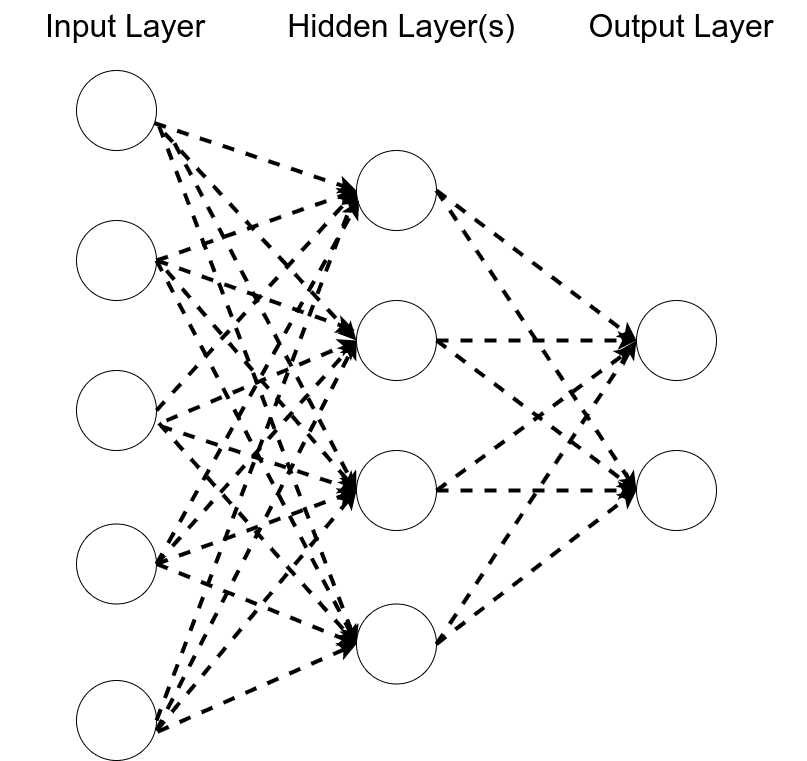
\includegraphics[width=0.45\textwidth]{background/images/neural-network.png}
  \caption{Basic artificial neural network structure.}\label{fig:neural-network}
  \vspace{-16mm}
\end{wrapfigure}

Artificial Neural Networks are systems that are based on the network of neurons of the animal brain \cite{mcculloch1943logical}. These neurons are called \textit{artificial neurons} and are referred to as \textit{nodes}. They are interconnected and organized in \textit{layers} to eventually form a neural network (see Fig. \ref{fig:neural-network}). Each node (represented by a circle) receives the information from the nodes in the previous layer and transmits the new information to the next layer. Input nodes are the exception because they already have the information. New information transmitted by the node is a value from its activation function after receiving all the inputs. The connection between two nodes modifies the output from the lower-layer node before entering the higher-layer node. Most of the networks have an additional bias value for each of the nodes, which can be seen as a regularization parameter. Neural networks have at least three layers: one input layer, one output layer, and at least one hidden layer. The output of the neural network can be defined as:

\begin{equation}\label{eq:forward-pass}
    z^l_j = \sigma \left( \sum_{i}^N(x_i^{l-1} *w_{i,j}^l) + b^l_j \right)
\end{equation}

\newpage

Where:

\begin{itemize}
    \item $l$ is a current layer
    \item $z_j^l$ is an output from the $j$th neuron in layer $l$
    \item $x_i^{l-1}$ is an output from the $i$th neuron on the $l-1$ layer (previous layer)
    \item $w_{i,j}^l$ is a weight for the pair of a current neuron at $j$th position and $i$th neuron from the previous layer
    \item $N$ is a number of neurons in the $l-1$ layer
    \item $b_j^l$ is a bias of $j$th neuron in layer $l$
    \item $\sigma$ is an activation function
\end{itemize}

The goal of a neural network is then finding the value of the weights $w_{ij}^l$ and the biases $b_j^l$ to generate the correct output. These values are optimized in the process called backpropagation.

\subsection{Backpropagation}

Backpropagation is an algorithm that calculates the changes to the weights of the network that are then used to update those weights. The process was first described by Paul Werbos in 1974 \cite{werbos1974beyond}. Even if the name "backpropagation" refers only to gradient computation, it is usually used to describe the whole process of updating the weights. This process consists of three parts. The first part is a feed-forward computation of the input (as defined above), then the error is calculated using the loss function, and lastly, based on the loss function with respect to the weights, the backpropagation computer the gradient used to update the weights.

\vspace{\baselineskip}

After the forward propagation, the error is calculated using a loss function $L(y,\hat{y})$ (where $\hat{y}$ is a predicted output and $y$ is a target output). Usually, the output of the network is a vector $\hat{y} \in \mathbb{R}^n$, and the loss function is a function that translates the difference between $y$ and $y$ into a real number, representing the "cost". One of the simplest loss functions is the Euclidean distance:

\begin{equation}
    L(y,\hat{y}) = \frac{1}{2} || \hat{y} - y  ||^2
\end{equation}

In order to update weights, the gradients have to be calculated with respect to these weights:

\begin{equation}
    \frac{\partial L}{\partial W_l}
\end{equation}

Where $W_l$ is a weight matrix at layer $l$. Computation of that gradient is difficult, but fortunately, the chain rule can be used. It is easier to explain the calculation when the forward function is split into parts (where $\text{CE}$ stands for \textit{Cross-Entropy} loss function defined in equation \ref{eq:cross-entropy}, often used for classification).

\begin{equation}
    z_1 = W_1x + b_1
\end{equation}
\begin{equation}\label{eq:activation-relu}
    h = \text{ReLU}(z_1)
\end{equation}
\begin{equation}
    z_2 = W_2h + b_2
\end{equation}
\begin{equation}
    \hat{y} = \text{sorfmax}(z_2)
\end{equation}
\begin{equation}
    L = \text{CE}(y, \hat{y})
\end{equation}

\begin{equation}\label{eq:cross-entropy}
    \text{CE}(y, \hat{y}) = -(y log(\hat{y}) + (1-y)log(1-\hat{y}))
\end{equation}


Gradient for $W_1$:

\begin{equation}
    \frac{\partial L}{\partial W_1} = \frac{\partial L}{\partial z_2}\frac{\partial z_1}{\partial W_1} = \left( (\hat{y} - y)^Tz_2 \circ sgn(h) \right)^T x^T
\end{equation}

And for $b_1$ :

\begin{equation}
    \frac{\partial L}{\partial w_1} = \frac{\partial L}{\partial z_2}\frac{\partial z_1}{\partial b_1} = \left( (\hat{y} - y)^Tz_2 \circ sgn(h) \right)^T
\end{equation}

Where $sgn$ is a sign function which is a derivative of the ReLU activation function (see eq. \ref{eq:relu-deriv}). With the value of the gradients, weights and biases can be updated.

\subsubsection*{ReLU}

\begin{wrapfigure}{R}{0.30\textwidth}
  \begin{tikzpicture}
    \begin{axis}[
        axis lines = left,
        xlabel = $x$,
        ylabel = {$f(x)$},
        width=0.3\textwidth,
        ymin = -1,
        ymax = 1,
        grid=both,
        legend pos=north east,
    ]
    %Here the blue parabloa is defined
    \addplot [
        domain=-1:1, 
        samples=100, 
        color=blue,
        ]
        {max(0, x)};
    
    \end{axis}
  \end{tikzpicture}
  \caption{$\text{ReLU}(x)$ where $x \in <-1,1>$}\label{fig:relu-example}
  \begin{tikzpicture}
    \begin{axis}[
        axis lines = left,
        xlabel = $x$,
        ylabel = {$f(x)$},
        width=0.3\textwidth,
        ymin = -1,
        ymax = 1,
        grid=both,
        legend pos=north east,
    ]
    %Here the blue parabloa is defined
    \addplot [
        domain=-1:1, 
        samples=100, 
        color=blue,
        ]
        {max(x/6, x)};
    
    \end{axis}
  \end{tikzpicture}
  \caption{$\text{Leaky ReLU}(x)$ where $x \in <-1,1>$}\label{fig:leaky-relu-example}
\end{wrapfigure}

As described in equation \ref{eq:forward-pass} and then later in \ref{eq:activation-relu}, the output is calculated with the use of the activation function. Usually that function is a ReLU function \cite{hahnloser2000digital}. ReLU stands for \textit{Rectified Linear Unit function} and is defined as:

\begin{equation}
    \text{ReLU}(x) = max(x,0)
\end{equation}

and visualized in Figure \ref{fig:relu-example}. Because ReLU returns $0$ every time the value of $x$ is less than $0$, it can deactivate neurons, and therefore create sparser networks. There are two issues with the ReLU function. The first one is that it can create "dead neurons" if all of the inputs of a neuron are less than zero. The second one is that it is not fully differentiable (at the $(0,1)$ point). The first one was solved by Mass et al. \cite{maas2013rectifier} by replacing a zero-valued tail of the ReLU with a slightly negative value $\alpha x$ (where $\alpha$ is a small positive number). Derivative of the ReLU function is defined as follow:

\begin{equation}\label{eq:relu-deriv}
    \text{ReLU}'(x) = \begin{cases} 1 & \text{if } x > 0 \\ 0 & \text{otherwise} \end{cases} = sgn(\text{ReLU}(x))
\end{equation}

\subsection{Convolutional Neural Networks}

Convolutional Neural Network (CNN) \cite{lecun1995convolutional, lecun1989backpropagation} are the type of Neural Networks with at least one convolutional layer. The first convolutional neural networks were LeNet \cite{cnnLecun1998} and AlexNet \cite{krizhevsky2012imagenet}, using only a few convolutional layers. CNNs are assuming that the input data consists of hierarchical patterns which can be used instead of relying on individual features and creating a connection between every single feature and neuron. This approach helps to reduce the number of parameters required by the network.

\subsubsection*{Convolutional Layer}

The convolutional layer uses the idea of filters/kernels with a given size and depth. A layer like that produces the output called a feature map, which is a combination of all the outputs from the kernels. As mentioned, each kernel is defined by the size (which corresponds to its width and height), depths (usually the depth of the input), and additional parameters like padding, stride, or dilatation. The name "convolutional" comes from the mathematical operation of convolution, which is denoted by $f*g$, and the output of that operation is a function that described how one function modifies the other. It can be defined as:

\begin{equation}
    g(m,n) = (h*f)(m,n) = \sum_{u} \sum_{v} h(u,v)f(m-u,n-v)
\end{equation}

Where $f$ is the input image, $h$ is the kernel, $m$ and $n$ are the corresponding row and column in the feature map, and $u$ and $v$ range over all legal subscripts for $h(u,v)$ and $f(m-u,n-v)$ \cite{keller2010convolutions}. An example of the convolution operation for the $m=0, n=3$ is shown in Figure \ref{fig:convolutional operation}.

\begin{figure}[ht]
    \centering
\begin{tikzpicture}[scale=1.0]

  \matrix [nodes=draw,column sep=-0.2mm, minimum size=6mm]
  {
    \node {0}; & \node{1}; & \node {1}; & \node{$1_{\times 1}$}; & \node{$0_{\times 0}$}; 
    & \node{$0_{\times 1}$}; & \node{0}; \\
    \node {0}; & \node{0}; & \node {1}; & \node{$1_{\times 0}$}; & \node{$1_{\times 1}$}; 
    & \node{$0_{\times 0}$}; & \node{0}; \\
    \node {0}; & \node{0}; & \node {1}; & \node{$1_{\times 1}$}; & \node{$1_{\times 0}$}; 
    & \node{$1_{\times 1}$}; & \node{0}; \\
    \node {0}; & \node{0}; & \node {1}; & \node{\, 1 \,}; & \node{\, 1 \, }; 
    & \node{\, 0 \,}; & \node{0}; \\
    \node {0}; & \node{0}; & \node {1}; & \node{\, 0 \, }; & \node{\, 0 \, }; 
    & \node{\, 0 \,}; & \node{0}; \\
    \node {0}; & \node{1}; & \node {0}; & \node{\, 0 \, }; & \node{\, 0 \, }; 
    & \node{\, 0 \,}; & \node{0}; \\
    \node {1}; & \node{1}; & \node {0}; & \node{\, 0 \,}; & \node{\, 0 \, }; 
    & \node{\, 0 \,}; & \node{0}; \\
  };


  % coordinates for coloring filter in array
  \coordinate (A) at (-0.6,0.3);
  \coordinate (B) at (1.78,0.3);
  \coordinate (C) at (1.78,2.12);
  \coordinate (D) at (-0.6,2.12);
  \fill[red, opacity=0.3] (A)--(B)--(C)--(D)--cycle;
  \begin{scope}[shift={(3.3,0)}]
    \node[] at (0,0) {\Large $\ast$};
  \end{scope}[shift={(2.5,0)}]

  \begin{scope}[shift={(5,0)}]

    %\matrix [matrix of math nodes,left delimiter={[},right
    %delimiter={]}]
    \matrix [nodes=draw,column sep=-0.2mm, minimum size=6mm]
    {
      \node{1};  & \node{0};   & \node{1};  \\
      \node{0};  & \node{1};   & \node{0};  \\
      \node{1}; & \node{0}; & \node{1}; \\
    };
    \coordinate (A1) at (-0.9,-0.9);
    \coordinate (B1) at (0.93,-0.9);
    \coordinate (C1) at (0.93,0.92);
    \coordinate (D1) at (-0.9,0.92);
    \fill[blue, opacity=0.2] (A1)--(B1)--(C1)--(D1)--cycle;
    \draw[blue, line width=2] (A1)--(B1)--(C1)--(D1)--cycle;
  \end{scope}

  \draw[dotted, line width=1, color=blue] (A)--(A1);
  \draw[dotted, line width=1, color=blue] (B)--(B1);
  \draw[dotted, line width=1, color=blue] (C)--(C1);
  \draw[dotted, line width=1, color=blue] (D)--(D1);

  \begin{scope}[shift={(6.6,0)}]
    \node[] at (0,0) {\Large $=$};
  \end{scope}[shift={(2.5,0)}]

  \begin{scope}[shift={(9,0)}]

    %\matrix [matrix of math nodes,left delimiter={[},right
    %delimiter={]}]
    \matrix [nodes=draw,column sep=-0.2mm, minimum size=6mm]
    {
      \node{1};  & \node{4};   & \node{3}; & \node{4}; & \node{1};  \\
      \node{l};  & \node{2};   & \node{4}; & \node{3}; & \node{3};  \\
      \node{1}; & \node{2}; & \node{3}; & \node{4} ; & \node{1};  \\
      \node{1}; & \node{3}; & \node{3}; & \node{1} ; & \node{1};  \\
      \node{3}; & \node{3}; & \node{1}; & \node{1} ; & \node{0};  \\
    };
    \coordinate (A2) at (0.3,0.9);
    \coordinate (B2) at (0.91,0.9);
    \coordinate (C2) at (0.91,1.507);
    \coordinate (D2) at (0.3,1.507);
    \fill[green, opacity=0.2] (A2)--(B2)--(C2)--(D2)--cycle;
    \draw[green, line width=2] (A2)--(B2)--(C2)--(D2)--cycle;
  \end{scope}

  \draw[dotted, line width=1, color=green] (A1)--(A2);
  \draw[dotted, line width=1, color=green] (B1)--(B2);
  \draw[dotted, line width=1, color=green] (C1)--(C2);
  \draw[dotted, line width=1, color=green] (D1)--(D2);
\end{tikzpicture}
    \caption{Example of the convolutional operation}
    \label{fig:convolutional operation}
\end{figure}

The standard convolutional layer uses multiple kernels at once, and every one of them has $\text{size} \times \text{size}$ learnable parameters. Putting that in a context where a fully connected neural network requires a weight for every pixel of the input image times the number of neurons in the hidden layer, a convolutional layer is a huge decrease in the total number of parameters. A kernel with a size of $3$ has $9$ learnable parameters. Even with having 50 kernels in the convolutional layer, there are only $450$ learnable parameters in total (for any input image size). For a $32\times32$ image, a fully connected layer with 10 neurons would require $10240$ parameters. It is worth noticing that kernels do not have to be square. The square is computationally efficient, but there were tries to use different shapes \cite{luo2019hexagonal, graham2015sparse, thomas2019kpconv}.

\subsubsection*{Pooling Layer}

CNNs have an additional type of layer called the \textit{Pooling Layer}. There are two types of pooling layers called: \textit{Max Pooling} and \textit{Average Pooling}. Each pooling layer is defined by its size (called the window size), and the result is based only on pixels from that window. The value returned by the max pooling layer is the maximum value from the window. The average pooling layer returns the average from all values from that window.

\begin{figure}[ht]
    \centering
    \begin{subfigure}{.49\textwidth}
        \begin{tikzpicture}[scale=0.7]
        \fill[yellow!20] (0,0) rectangle (2,2);
        \fill[red!20] (0,2) rectangle (2,4);
        \fill[green!20] (2,2) rectangle (4,4);
        \fill[blue!20] (2,2) rectangle (4,0);
        %...
        \draw[gray,very thin] (0,0) grid (4,4);
        \node at (0.5,0.5) {1};
        \node at (1.5,0.5) {2};
        \node at (2.5,0.5) {3};
        \node at (3.5,0.5) {1};
        \node at (0.5,1.5) {3};
        \node at (1.5,1.5) {4};
        \node at (2.5,1.5) {0};
        \node at (3.5,1.5) {7};
        \node at (0.5,2.5) {2};
        \node at (1.5,2.5) {6};
        \node at (2.5,2.5) {8};
        \node at (3.5,2.5) {5};
        \node at (0.5,3.5) {1};
        \node at (1.5,3.5) {4};
        \node at (2.5,3.5) {2};
        \node at (3.5,3.5) {7};
        %...
        \draw[-stealth,ultra thick] (5,2) --node[above] { 2x2 avg. pool} (7,2);
        \draw[gray,very thin] (8,1) grid (10,3);
        \fill[yellow!20] (8,1) rectangle (9,2);
        \fill[red!20] (8,2) rectangle (9,3);
        \fill[green!20] (9,2) rectangle (10,3);
        \fill[blue!20] (9,1) rectangle (10,2);
        \node at (8.5,1.5) {2.5};
        \node at (9.5,1.5) {2.7};
        \node at (8.5,2.5) {3.2};
        \node at (9.5,2.5) {6.2};
        
        \end{tikzpicture}
    \caption{Average Pooling}
    \label{fig:cnn-avg-pooling}
    \end{subfigure}
    \begin{subfigure}{.49\textwidth}
        \begin{tikzpicture}[scale=0.7]
        \fill[yellow!20] (0,0) rectangle (2,2);
        \fill[red!20] (0,2) rectangle (2,4);
        \fill[green!20] (2,2) rectangle (4,4);
        \fill[blue!20] (2,2) rectangle (4,0);
        %...
        \draw[gray,very thin] (0,0) grid (4,4);
        \node at (0.5,0.5) {1};
        \node at (1.5,0.5) {2};
        \node at (2.5,0.5) {3};
        \node at (3.5,0.5) {1};
        \node at (0.5,1.5) {3};
        \node at (1.5,1.5) {4};
        \node at (2.5,1.5) {0};
        \node at (3.5,1.5) {7};
        \node at (0.5,2.5) {2};
        \node at (1.5,2.5) {6};
        \node at (2.5,2.5) {8};
        \node at (3.5,2.5) {5};
        \node at (0.5,3.5) {1};
        \node at (1.5,3.5) {4};
        \node at (2.5,3.5) {2};
        \node at (3.5,3.5) {7};
        %...
        \draw[-stealth,ultra thick] (5,2) --node[above] { 2x2 max pool} (7,2);
        \draw[gray,very thin] (8,1) grid (10,3);
        \fill[yellow!20] (8,1) rectangle (9,2);
        \fill[red!20] (8,2) rectangle (9,3);
        \fill[green!20] (9,2) rectangle (10,3);
        \fill[blue!20] (9,1) rectangle (10,2);
        \node at (8.5,1.5) {4};
        \node at (9.5,1.5) {7};
        \node at (8.5,2.5) {6};
        \node at (9.5,2.5) {8};
        
        \end{tikzpicture}
    \caption{Max Pooling}
    \label{fig:cnn-max-pooling}
    \end{subfigure}
    \caption{Example of pooling layers results applied to the same $4 \times 4$ feature map. Colors indicate the area from which the values are pulled to produce the result.}
    \label{fig:cnn-pooling}
\end{figure}
\section{Interpretability}\label{section:interpretability-def}

There is no one formal definition of interpretability and/or explainability in the context of machine learning, and often it is used interchangeably \cite{guidotti2018survey}. Arrieta et al. \cite{arrieta2020explainable} distinguish between the two and define them as:

\begin{definition}[Interpretability]\label{def:interpretability}
Passive characteristic on a model refers to the level of understanding of the models' internal decision process for a human observer.
\end{definition}

\begin{definition}[Explainability]\label{def:explainability}
Active characteristic of a model, associated with the notion of explanation of the action or procedure taken by the model with the intent of clarifying its internal decision process.
\end{definition}

The name of the field Explainable Artificial Intelligence (XAI) refers to the characteristic of a model, but any representation presented to the human (like input attribution) refers to the interpretability of the model. This thesis focuses on the interpretability of CNNs and uses the taxonomy of interpretability as defined in Figure \ref{fig:taxonomy-interpretability} \cite{lipton2018mythos}.

\subsection{Taxonomy of interpretability}\label{section:taxonomy-xai}

\begin{figure}[ht]
    \centering
\begin{tikzpicture}[sibling distance=10em,
  every node/.style = {shape=rectangle,
    draw, align=center,
    top color=white, bottom color=white}]]
  \node  {Model Interpretability}
      child { node {Post-hoc}
        child { node {Model-Agnostic} }
        child { node {Model-Specific} } }
      child { node {Intrinsic} };
\end{tikzpicture}
    \caption{Taxonomy of the model interpretability.}
    \label{fig:taxonomy-interpretability}
\end{figure}

There are two major types of models: \textit{white-box models} and \textit{black-box models}. Interpretability of the first type is defined as the \textit{Intrinsic} \cite{biran2017explanation}. This type of interpretability covers all models which have an interpretable internal structure. As an example, the structure of a decision tree is considered interpretable, as well as the internal structure of a shallow neural network. This does not apply to deep neural networks where \textit{post-hoc} interpretability is used. The post-hoc interpretability means that we are trying to explain a prediction of the model without explaining the exact internal mechanism of that model. Because of the complexity of CNNs, post-hoc interpretability is the only way to interpret this kind of model.

\begin{remark}
This is not the only taxonomy of interpretability. The structure of the interpretability can be defined in many ways (either by the purpose, by the method, or by the application).
\end{remark}

\subsubsection*{Model-Agnostic and Model-Specific}

As shown in the taxonomy (see Fig. \ref{fig:taxonomy-interpretability}), post-hoc interpretability is divided into \textit{model-agnostic} and \textit{model-specific} \cite{adadi2018peeking}. The model-agnostic methods are the methods that can be applied to any black-box model without the concern about the internal structure of the model. These methods are usually less precise but because they explain the models' behavior only based on the input and the output. On the other hand, model-specific methods are associated with a particular type of model. The "type" is loosely defined and can refer to the whole domain like CNNs or the specific architecture of CNN. In this thesis, both types of post-hoc interpretability are used.

\subsection{Right to explanation}

The "right to explanation" is a term used by the European Parliament and Council in the General Data Protection Regulation (GDPR) \footnote{Reg (EU) 2016/679 of the European Parliament and of the Council of 27 April 2016 on the protection of natural persons with regard to the processing of personal data and on the free movement of such data, and repealing Dir 95/46/EC (General Data Protection Regulation) 2016.}. This term is often mentioned in regard to XAI methods and requires a data controller to explain how the mechanism reached a decision. This part of the GDPR was created with an intent to prevent using the systems what decision cannot be interpreted by the human (like deep neural networks). The goal is to avoid discrimination and ethical/financial biases in such systems. As an example, we can use the automated credit scoring system. Systems like that are used in the mortgage loan process. It is legally forbidden to discriminate against a person base on a list of characteristics, but that discrimination can be hidden inside a black-box system (even without the knowledge of the creator of that system). If the application is refused by the bank, the applicant can require an explanation of why it was refused. This might help to potentially improve the score before the next application.

\section{Attribution Methods}


Attribution methods are one of the types of post-hoc methods (see section \ref{section:taxonomy-xai}). Attribution methods, as the name says, attribute the input features to a given prediction. It can be defined as:

\begin{definition}[Attribution method]\label{def:attribution-method}
Given an input vector $x \in \mathbb{R}^n$ where $n$ represents the number of dimensions, class $C$ and the model $F: \mathbb{R}^{n} \rightarrow \mathbb{R}^C$. The attribution method is defined as $A(F, x, C): \mathbb{R}^{n} \rightarrow \mathbb{R}^{n}$. Provided explanation corresponds to the "importance" of an element from the input vector for a given \textit{class} $C$ and \textit{model} $F$.
\end{definition}

This definition can be rewritten to fit the input of the usual Convolutional Neural Network with the $m \times n$ input matrix:

\begin{definition}[Attribution method - CNN]\label{def:attribution-method-cnn}
Given an input matrix $x \in \mathbb{R}^{m \times n}$ where $m \times n$ represents the dimensions of the input, class $C$ and the model $F: \mathbb{R}^{m \times n} \rightarrow \mathbb{R}^C$. The attribution method is defined as $A(F, x, C): \mathbb{R}^{m \times n} \rightarrow \mathbb{R}^{m \times n}$. Provided explanation corresponds to the "importance" of an element from the input matrix for a given \textit{class} $C$ and \textit{model} $F$.
\end{definition}

\begin{wrapfigure}{R}{0.50\textwidth}
  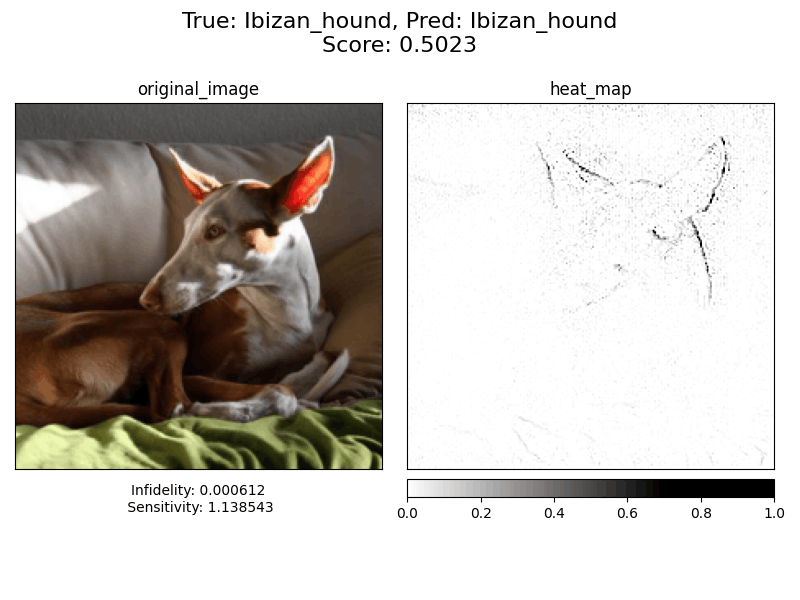
\includegraphics[width=0.50\textwidth]{background/images/1280-Ibizan_hound-Ibizan_hound.png}
  \caption{Visualization of the attribution by the Guided GradCAM generated for the class \textit{ibizan\_hound}. Image source: \textit{Stanford Dogs} \cite{stanford-dogs}}\label{fig:gradcam-ibizan-hound}
  \vspace{-30mm}
\end{wrapfigure}


To better visualize the attribution, we can look at Figure \ref{fig:gradcam-ibizan-hound}. For predicting a class of \textit{ibizan\_hound}, each pixel of the input image was given a value that defined its attribution to the prediction. Pixels (features) with higher attribution could be considered "more important" in predicting that class. We can see that the pixels with the highest attribution values are the pixels at the edges of the dog's head and ears. 

\vspace{\baselineskip}

As in the case of interpretability versus explainability (section \ref{section:interpretability-def}), the is a lack of agreement on vocabulary. Attribution methods are often known as \textit{saliency methods}, \textit{feature relevance}, \textit{feature importance}, \textit{heatmaps}, \textit{neuron activations}, and \textit{saliency masks}.

\newpage

\section{Quantitative and Qualitative research}

The type of research can be divided into qualitative or quantitative \cite{creswell2002educational}. The qualitative type of research is often related to the observation and processing of non-numerical data. The contrast to qualitative research is called quantitative research, and  it relies on the numerical analysis of collected data. Interpretability of machine learning models is a human-centric field of study. That is why most of the XAI method researchers base their solutions on qualitative measures rather than quantitative ones. This thesis argues that the current qualitative approach can prone to errors.

\subsection{Qualitative measures}

In qualitative research, the data is collected through observation, pools, or interviews. This kind of data is very subjective and related to the person providing the data. An example of such a subjective measure is shown in Figure \ref{fig:attr-comparison}. If presented with two attributions for the same input image, the decision of which one is better may change with the person. This is even more likely when two attributions have similar "quality". 

\begin{figure}[h]
  \centering
 \begin{subfigure}{.23\textwidth}
    \centering
    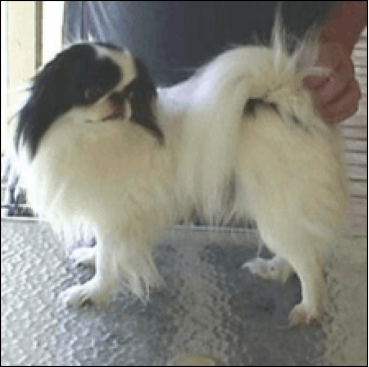
\includegraphics[width=\textwidth]{background/images/org-Japanese_spaniel.png}
    \caption{Input data}\label{fig:attr-comparision-image}
\end{subfigure}
 \begin{subfigure}{.23\textwidth}
    \centering
    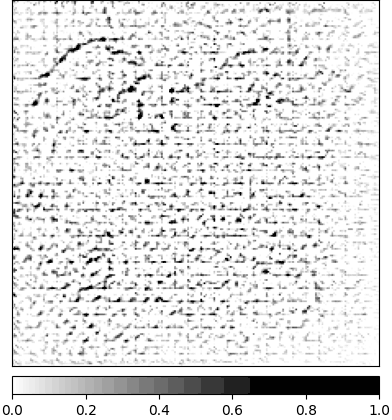
\includegraphics[width=\textwidth]{background/images/deconv-Japanese_spaniel.png}
    \caption{Attribution 1}\label{fig:attr-comparision-deconv}
\end{subfigure}
 \begin{subfigure}{.23\textwidth}
    \centering
    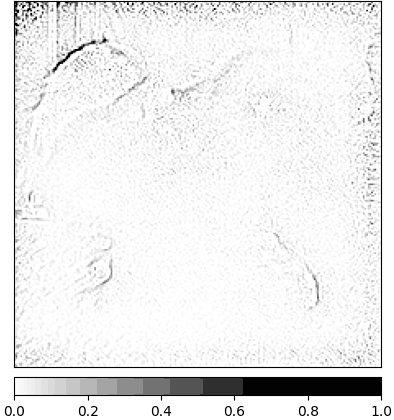
\includegraphics[width=\textwidth]{background/images/gbpJapanese_spaniel.png}
    \caption{Attribution 2}\label{fig:attr-comparision-gbp}
\end{subfigure}

 \caption{Comparison of attributions from two different methods for the same input data. Both attributions are generated for the same model with different XAI methods. Image source: \textit{Stanford Dogs} \cite{stanford-dogs} }\label{fig:attr-comparison}
\end{figure}

The results of the qualitative measures cannot be compared with each other without the specific context and prior knowledge about the data producers. Even with that knowledge, comparing the results might be difficult. The same issue applies to reproducibility, were to repeat the measurement, we have to be sure that all the participants are going to give the same answer. Another problem with qualitative measures is their scalability. Because most of the methods rely on human input, to measure the same method again or to compare it with another method, we have to repeat the work twice.

\subsection{Quantitative measures}

The data in the quantitative research is stored in a numeric form. This numeric form has to be comparable with other data measured in the same way. Each measurement is repeatable, and when done once, it can be reused all over again. This type of research has a huge advantage over qualitative research because of its scalability. The problem with qualitative measurement is that we have to define the measure to return meaningful results. Defining a measure of human visual perception is a difficult task, and the measure itself should be objective, which is even harder when trying to measure complex things like attributions. Having such a measure allows us to easily compare and reproduce experiments.

\newpage

\section{Related work}

Ghorbani et al. \cite{ghorbani2019interpretation} discuss attacks using adversarial perturbations to produce different interpretations of the same image. Their paper shows that we can generate such adversarial perturbations that produce perceptively indistinguishable inputs with the same prediction, but the attribution differs by a considerable margin from the original attribution. This thesis also focuses on the effect of input perturbation, but instead of searching for adversarial perturbation, it applies augmentations that aim to simulate real-world image processing that happens in modern cameras and check how they influence attribution.

\vspace{\baselineskip}

Another approach to the influence of perturbation on interpretability was taken by Kindermans et al. \cite{kindermans2016investigating}. They have studied the effect of applying noise to the input image and what effect it has on the explanation provided by the methods available at that time.

\vspace{\baselineskip}

One of the most influential papers on the subject was done by Adebayo et al. \cite{adebayo2018sanity} in 2018. Their work examined the influence of noise on the gradient values on different layers in the CNN. This was done by checking the correlation between the value of the gradient before and after applying the noise. The check was performed using multiple similarity metrics. Their work proved that gradients could be influenced by simple noise.

\vspace{\baselineskip}

Hooker et al. \cite{hooker2018benchmark} were one of the first who tried to measure the XAI methods quantitatively. The exact framework used is described in section \ref{section:roar}. The study assumed that if after removing pixels attributed as important to the prediction and retraining the model, the model still performs well, then the attribution is wrong. This approach might be logical, but it is extremely computationally expensive and therefore useless in real-world scenarios when there are limited resources.
	\cleardoublepage

	\chapter{Attribution Methods}\label{chapter:methods}
\thispagestyle{chapterBeginStyle}

\vspace{-20mm}
\section{Deconvolution}\label{section:deconvolution}

The idea of Deconvolution \cite{zeiler2013visualizing} comes from the work of Zeiler et al. \cite{zeiler2011adaptive} about \textit{Deconvolutional Networks (\textit{deconvnets}}. Deconvnets are designed to work similar to convolutional networks but reverse (reversing pooling component, reversing filter component etc.), and they can be trained using an unsupervised approach. In a deconvolutional approach to explaining the model, we are not training a deconvnet but rather probe our CNN with it. 

\begin{wrapfigure}{R}{0.4\textwidth}
\vspace{-1.5\baselineskip}
\centering
  \setlength{\belowcaptionskip}{12pt}
  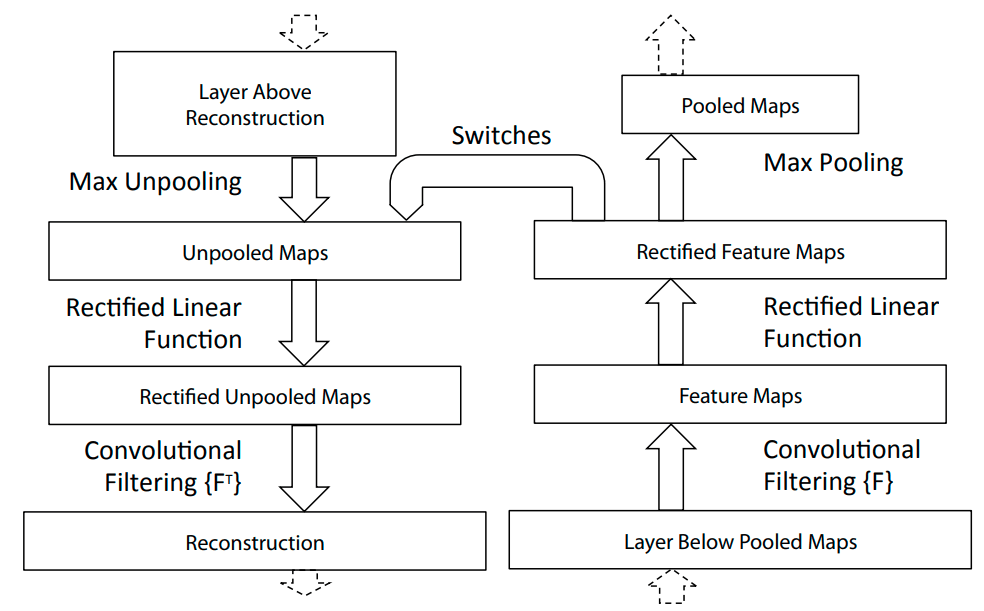
\includegraphics[width=0.4\textwidth]{methods/images/deconv-layer.png}
  \caption{A deconvnet layer (left) attached to a CNN layer (right), source \cite{zeiler2013visualizing}}\label{fig:deconvolution-layer}
  \setlength{\belowcaptionskip}{12pt}
  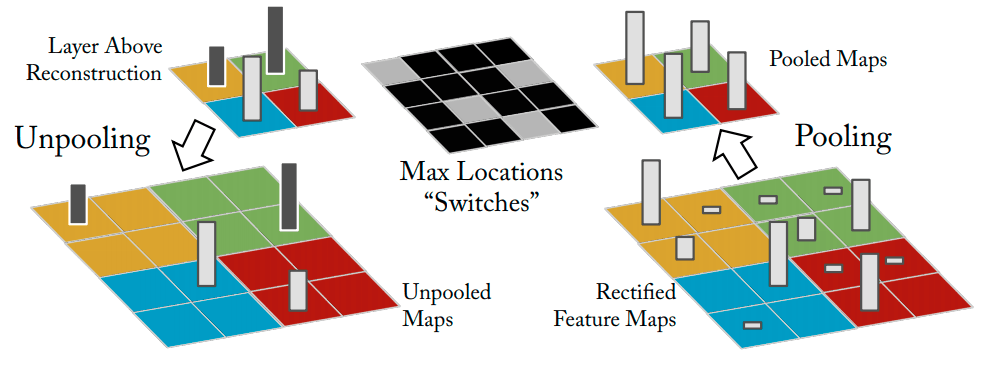
\includegraphics[width=0.4\textwidth]{methods/images/deconv-layer-unpooling.png}
  \caption{The unpooling layer, source \cite{zeiler2013visualizing}}\label{fig:deconvolution-layer-unpooling}
  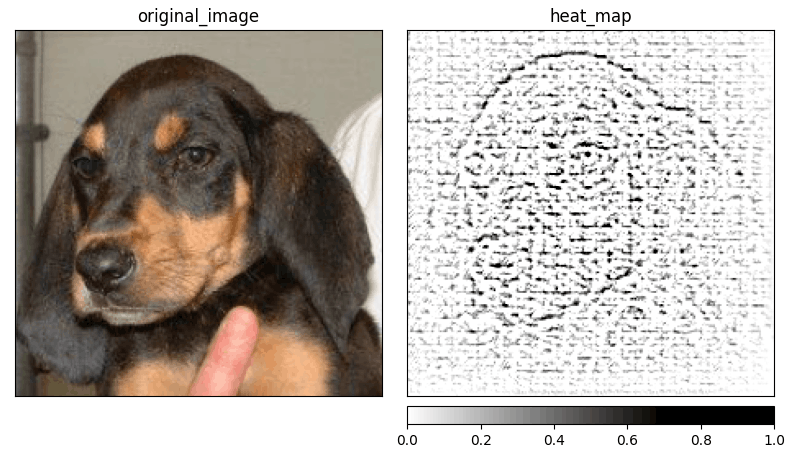
\includegraphics[width=0.35\textwidth]{methods/images/deconv-black-and-tan-coonhound.png}
  \caption{Visualization of the saliency map generated by deconvolution for the class \textit{black-and-tan-coonhound}. Image source: \textit{Stanford Dogs} \cite{stanford-dogs}}\label{fig:saliency-map-coonhound}
    \vspace{-\baselineskip}
\end{wrapfigure}

\vspace{\baselineskip}

To reconstruct the activation on a specific layer, we are attaching \textit{deconv layers} to corresponding \textit{CNN layers} (see Fig. \ref{fig:deconvolution-layer}). Then an image is passed through the CNN, and the network computes the output. To examine a reconstruction for a given class $c$, we have to set all activations except the one responsible for predicting class $c$ to zero. Then we can propagate through deconvnet layers and pass all the feature maps as inputs to corresponding layers.

\vspace{\baselineskip}

To calculate the reconstruction, deconvnet layer has to be able to reverse operations performed by the CNN layers. Authors designed specific components to compote the reverse operations done by CNN layers:

\vspace{\baselineskip}

\textbf{Filtering} in the original CNN computes \textit{feature maps} using learned filters. Reversing that operation requires the use of a transposed version of the same filters. Those transposed filters are then applied to the \textit{Rectified Unpooled Maps}.

\vspace{\baselineskip}


\textbf{Rectification} uses the same \textit{ReLU} non-linearity \cite{hahnloser2000digital} to compute \textit{Rectified Unpooled Maps} as it is used in CNN. It is simply just rectifying the values and propagate only non-negative ones to the \textit{filtering} layer.

\vspace{\baselineskip}

\textbf{Unpooling} corresponds to the \textit{Pooling Layer} of CNN (see Fig. \ref{fig:deconvolution-layer-unpooling}). The original max-pooling operation is non-invertible, but this approach uses additional variables called \textit{switch variables}, which are responsible for remembering the locations of the maxima for each pooling region. The unpooling layer uses these variables to make a reconstruction into the same locations as when the pooling was calculated.

\vspace{\baselineskip}

Propagation through the whole deconvnet gives us a representation of the features from the first layer of the original CNN (the last deconvnet layer corresponds to the first CNN layer). This approach causes the saliency map to feature some biases from the first convolutional layer and the representation looks like a localized edge detector (see Fig. \ref{fig:saliency-map-coonhound}). It usually works better when there is a clear distinction in the feature importance rather than similar values for the whole image.
\section{Saliency}\label{section:saliency}

Saliency \cite{simonyan2014deep} is one of the first attribution methods designed to visualize the input attribution of the Convolutional Network. Because the word \textit{saliency} is often related to the whole approach to display input attribution called \textit{Saliency Map}, this method is also known as \textit{Vanilla Gradient}.

\vspace{\baselineskip}

The idea of the Saliency method starts from the class visualization by finding $L_2\text{-regularized}$ image $I$ that maximizes score $S_c$ for a given class $c$. It can be written formally as:

\begin{equation}
\arg \max _{I} S_{c}(I)-\lambda\|I\|_{2}^{2}
\label{eq:saliency-image-maximization}
\end{equation}

\begin{wrapfigure}{R}{0.40\textwidth}
  \setlength{\belowcaptionskip}{-12pt}
  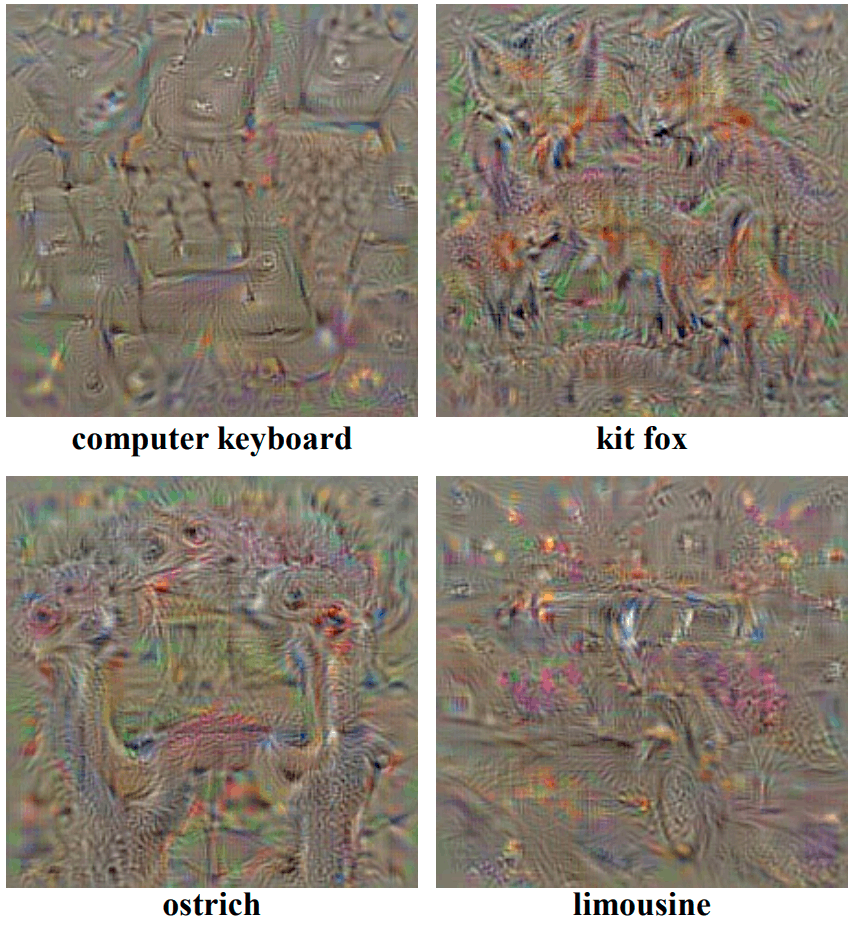
\includegraphics[width=0.40\textwidth]{methods/images/saliency-class-image-visualization.png}
  \caption{The class model visualizations for several classes, source \cite{simonyan2014deep}}\label{fig:saliency-class-image-visualization}
\end{wrapfigure}

Where $\lambda$ is a regularisation parameter. To find the value of $I$, we can use the back-propagation method. Unlike in the standard learning process, we are going to back-propagate with respect to the input image, not the first convolution layer. This optimization allows us to produce images that visualize a particular class in our model (see Fig. \ref{fig:saliency-class-image-visualization}).

\vspace{\baselineskip}

This idea can be extrapolated, and with minor modifications, we should be able to query for spatial support of class $c$ in a given image $I_0$. To do this, we have to rank pixels of $I_0$ in relation to their importance in predicting score $S_c(I_0)$. Authors assume that we can approximate $S_c(I)$ with a linear function in the neighborhood of $I_0$ with:

\begin{equation}
S_{c}(I) \approx w^\intercal I + b
\label{eq:saliency-class-score-approximation}
\end{equation}

where $w$ is a:

\begin{equation}
w=\left.\frac{\partial S_{c}}{\partial I}\right|_{I_{0}}
\label{eq:saliency-class-score-derivate}
\end{equation}

For a pair of input image $I_0 \in \mathbb{R}^{m \times n}$ and the class $c$, we are able to compute saliency map $A \in \mathbb{R}^{m \times n}$ (where $m$ and $n$ are the height and width of the input in pixels). All we have to do is to compute derivative $w$ (\ref{eq:saliency-class-score-derivate}) and rearrange elements in the returned vector.

\vspace{\baselineskip}

This method uses different approaches base on the number of channels in the input image $I_0$. For grey-scale pixels (one color channel), we can rearrange the pixels to match the shape of the image. If the number of channels is greater than one, we are going to use the maximum value from each set of values related to the specified pixel.


\begin{wrapfigure}{L}{0.30\textwidth}
  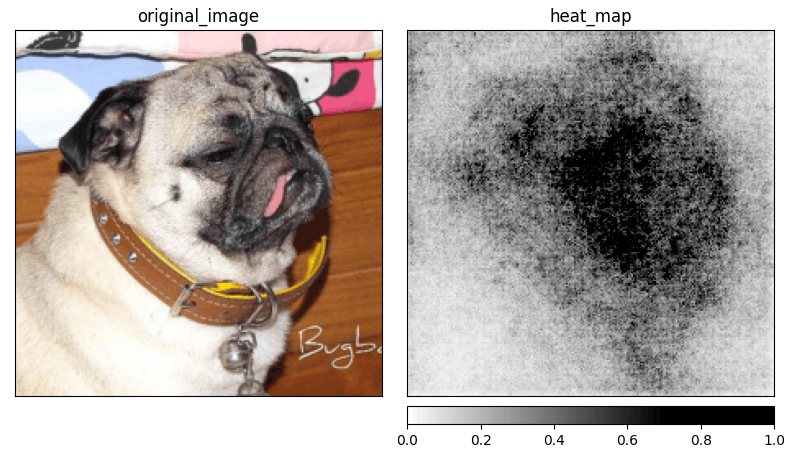
\includegraphics[width=0.30\textwidth]{methods/images/pug-saliency.png}
  \caption{Visualization of the saliency map by the Saliency generated for the class \textit{pug}. Image source: \textit{Stanford Dogs} \cite{stanford-dogs}}\label{fig:saliency-map-pug}
\end{wrapfigure}

\begin{equation}
A_{i,j} = \max _{ch}|w_{h(i,j,ch}|
\label{eq:saliency-rgb-map-generation}
\end{equation}

where $ch$ is a color channel of the pixel $(i,j)$ and $h(i,j,ch)$ is an index of the $w$ corresponding to the same pixel $(i,j)$. With the obtained map, we can visualize pixel importance for the input image $I_0$ as shown in the Figure \ref{fig:saliency-map-pug}.

\vspace{\baselineskip}

The original \textit{Saliency} method produces a lot of additional noise but still gives us an idea of which part of the input image is relevant when predicting a specific class. This often causes a problem when the object on the image has a lot of details and the model is using most of them to make a prediction.
\section{Guided Backpropagation}\label{section:gbp}

Guided Backpropagation (GBP) \cite{springenberg2014striving} is an approach designed by Springenberg et al., relying on the ideas of \textit{Deconvolution} (Section \ref{section:deconvolution}) and \textit{Saliency} (Section \ref{section:saliency}). Authors argue that the approach taken by Simonyan et al. \cite{simonyan2014deep} has an issue with the flow of negative gradients, which decreases the accuracy of the higher layers we are trying to visualize. Their idea is to combine two approaches and add a "guide" to the \textit{Saliency} with the help of deconvolution.

\vspace{\baselineskip}

To achieve that, we have to focus on the \textit{ReLU} activation function in the CNN. When computing values at the \textit{Rectification} component of the \textit{deconvnet}, we are masking all non-positive values with the \textit{ReLU}. In that layer, the computed values are calculated only base on the top signal (reconstruction from the upper layer), and the input is ignored. On the other hand, in the \textit{Saliency} method, we are focusing on the gradient values computed base on the input image. If we take deconvnet masking of the \textit{Rectification} layer and apply it on the gradient values of the \textit{Saliency} method, we could remove noise caused by the negative gradient values. This noise removal is the reason why the method has the prefix "guided". Deconvolution guides backpropagation values of the \textit{Saliency} method to produce sharper images (Fig. \ref{fig:gbp-gbp-attribution}).

\begin{figure}[h]
  \centering
 \begin{subfigure}{.2\textwidth}
    \centering
    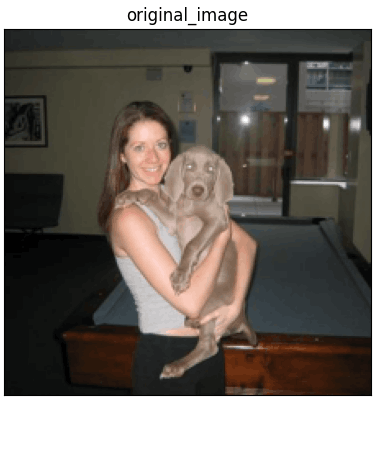
\includegraphics[width=\textwidth]{methods/images/Weimaraner-image.png}
    \caption{Original image}\label{fig:gbp-weimaraner}
\end{subfigure}
 \begin{subfigure}{.25\textwidth}
    \centering
    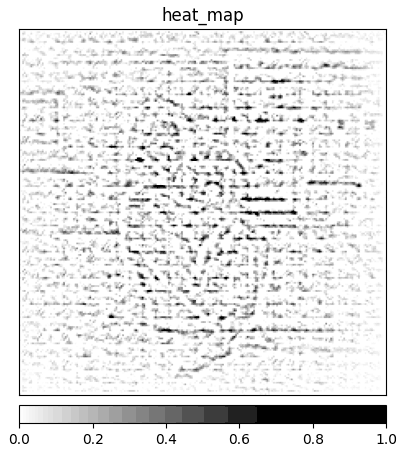
\includegraphics[width=\textwidth]{methods/images/1-4-0-rotation-30-Weimaraner-Weimaraner.png}
    \caption{Deconvolution results}\label{fig:gbp-deconv-attributione}
\end{subfigure}
 \begin{subfigure}{.25\textwidth}
    \centering
    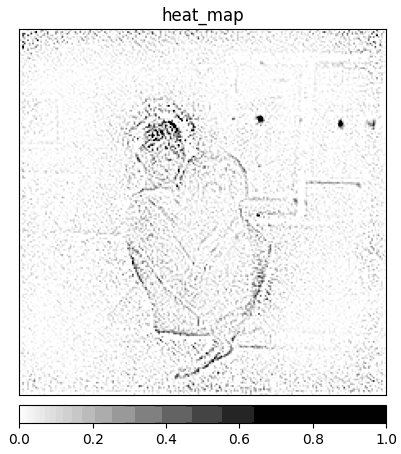
\includegraphics[width=\textwidth]{methods/images/1-4-0-rotation-30-Weimaraner-Weimaraner-gbp.png}
    \caption{GBP results}\label{fig:gbp-gbp-attribution}
\end{subfigure}
 \begin{subfigure}{.25\textwidth}
    \centering
    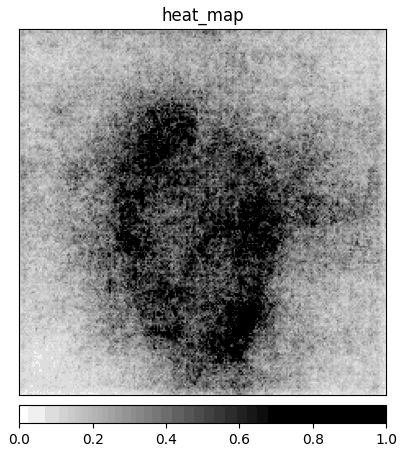
\includegraphics[width=\textwidth]{methods/images/1-4-0-rotation-30-Weimaraner-Weimaraner-saliency.png}
    \caption{Saliency results}\label{fig:gbp-saliency-attribution}
\end{subfigure}

 \caption{Visualisation of saliency maps produced by \textit{Saliency} (\ref{fig:gbp-saliency-attribution}), \textit{Deconvolution} (\ref{fig:gbp-comparision-with-deconv-and-saliency}), and \textit{GBP} (\ref{fig:gbp-gbp-attribution}) of the same input image \ref{fig:gbp-weimaraner} for a class \textit{weimaraner}. All the maps are generated using the same model (ResNet18). Image source: \textit{Stanford Dogs} \cite{stanford-dogs} }\label{fig:gbp-comparision-with-deconv-and-saliency}
\end{figure}

As we can see in Figure \ref{fig:gbp-comparision-with-deconv-and-saliency}, the use of the "guide" significantly reduces the amount of noise generated by the \textit{Saliency} method (Fig. \ref{fig:gbp-saliency-attribution}). The idea of GBP is often misunderstood and interpreted as "applying deconvolution results on the saliency results". This is not true because \textit{ReLU} masking extracted from the deconvnet is applied on every level and therefore affecting the gradient values all the way down to the input of the CNN, not only at the first level of the CNN. 
\section{Integrated Gradients}\label{section:ig}

Integrated Gradients (IG) \cite{sundararajan2017axiomatic} is a method proposed by Sundararajan et al. that bases on two axioms: \textit{Sensitivity} and \textit{Implementation Invariance}. Authors argue that those two axioms should be satisfied by all attribution methods. The definition of those two axioms is as follows:

\begin{definition}[Axiom: Sensitivity]\label{axiom:sensitivity}
An attribution method satisfies \textit{Sensitivity} if for every input and baseline that differ in one feature but have different predictions, then the differing feature should be given a non-zero attribution. If the function implemented by the deep network does not depend (mathematically) on some variable, then the attribution to that variable is always zero.
\end{definition}

\begin{definition}[Axiom:  Implementation Invariance]\label{axiom:implementation-invariance}
Two networks are functionally equivalent if their outputs are equal for all inputs, despite having very different implementations. Attribution methods should satisfy Implementation Invariance, i.e., the attributions are always identical for two functionally equivalent networks.
\end{definition}

The sensitivity axiom introduces the \textit{baseline} which is an important part of the IG method. Baseline is defined as an \textit{absence of feature} in an input. This definition is confusing, especially when dealing with complex models, but the baseline could be interpreted as \textit{"input from the input space that produces a neutral prediction"}. A baseline can be treated as an input to produce a counterfactual explanation by checking how the model behaves when moving from baseline to the original image.

\begin{remark}
The authors give the example of the baseline for an object recognition network, which is a black image. I personally think that a black image doesn't represent an "absence of feature", because this absence should be defined based on the manifold that represents data. This means that a black image could work as an absence of a feature in one network but may not work for a network trained on a different dataset, allowing a network to use black pixels in prediction.
\end{remark}


\begin{wrapfigure}{R}{0.30\textwidth}
  \begin{tikzpicture}
    \begin{axis}[
        axis lines = left,
        xlabel = $x$,
        ylabel = {$f(x)$},
        width=0.3\textwidth,
        ymax = 1.5,
        grid=both,
        legend pos=north east,
    ]
    %Here the blue parabloa is defined
    \addplot [
        domain=0:2, 
        samples=100, 
        color=blue,
        ]
        {1 - max(0, 1- x)};
    
    \end{axis}
    \end{tikzpicture}
  \caption{Values of $f(x) = 1 - \text{ReLU}(1 - x)$ where $x \in <0,2>$}\label{fig:ig-relu-example}
\end{wrapfigure}

Authors argue that gradient-based methods are violating Sensitivity (Def. \ref{axiom:sensitivity}). As an example, we are presented with the case of simple function, $f(x) = 1 - \text{ReLU}(1 - x)$ (see Fig. \ref{fig:ig-relu-example}) and the baseline being $x = 0$. When trying to generate attribution for $x = 2$, the functions' output changes from 0 to 1 but after $x=1$, it becomes flat and causes the gradient to equal zero. Obviously, $x$ attributes to the result, but because the function is flat at the input we are testing results in invalid attribution and breaks the Sensitivity. Sundararajan et al. think that breaking Sensitivity causes gradients to focus on irrelevant features.

\vspace{\baselineskip}

In IG definition we have a function $F$ representing our model, input $x \in \mathbb{R}^{n}$ ($x$ is in $\mathbb{R}^n$ because this is a general definition of IG and not CNN specific), and the baseline $x' \in \mathbb{R}^{n}$. We assume straightline path between $x$ and $x'$ and compute gradients long that path. The integrated gradient along $i^th$ dimension is defined as:

\begin{equation}
    IntegratedGrads_{i}(x) ::= (x_{i} - x'_{i})\times\int_{\alpha=0}^1\frac{\partial F(x'+\alpha \times (x - x'))}{\partial x_i}{d\alpha}
    \label{eq:ig-full-eq}
\end{equation}

The original definition of Integrated Gradients is incalculable (because of integral). Therefore, the implementation of the method uses approximated value by replacing the integral with summation:

\begin{equation}
    IntegratedGrads^{approx}_{i}(x)::=(x_{i}-x'_{i})\times\sum_{k=1}^{m}\frac{\partial F(x' + \frac{k}{m}\times(x - x'))}{\partial x_{i} } \times \frac{1}{m}
    \label{eq:ig-aprox}
\end{equation}

In the approximated calculation (Eq. \ref{eq:ig-aprox}), $m$ defines a number of interpolation steps. As an example, we can visualize the interpolations with $m$ equals five (see Fig. \ref{fig:ig-interpolation}). In practice, the number of interpolation steps is usually between 20 and 300, but the mode value is equal to 50. The results of applying IG can be seen in Figure \ref{fig:ig-saliency-map-bernard}.

\begin{figure}[ht]
    \centering
    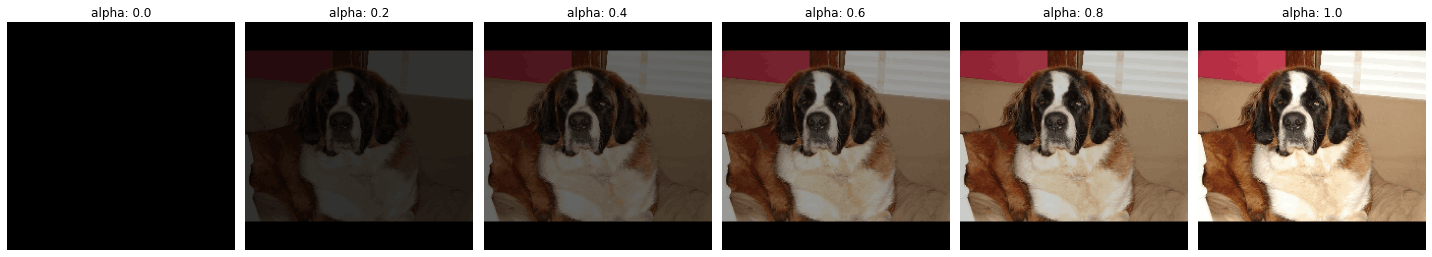
\includegraphics[width=\textwidth]{methods/images/ig-saint_bernard-interpolation.png}
 \caption{Five-step interpolation between the baseline $x'$ and the input image $x$. The first image on the left ($\text{alpha:} 0.0$) is not a part of the interpolation process. Image source: \textit{Stanford Dogs} \cite{stanford-dogs} }\label{fig:ig-interpolation}
\end{figure}

\begin{wrapfigure}{L}{0.30\textwidth}
  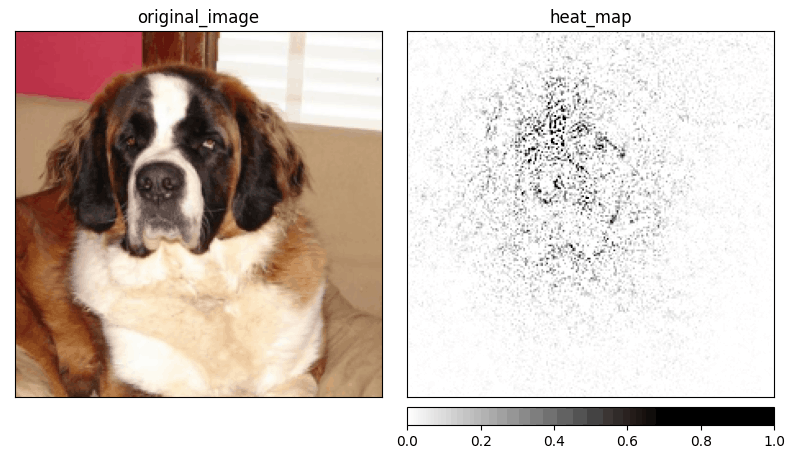
\includegraphics[width=0.30\textwidth]{methods/images/ig-saint_bernard.png}
  \caption{Visualization of the saliency map by the IG generated for the class \textit{saint\_bernard}. The result is averaged over 50 interpolation steps. Image source: \textit{Stanford Dogs} \cite{stanford-dogs}}\label{fig:ig-saliency-map-bernard}
\end{wrapfigure}

In recent years there was discussion about replacing constant color baseline with an alternative. One of the first propositions was to add Gaussian noise to the original image (see Fig. \ref{fig:ig-baseline-gaussian}. \textit{Gaussian baseline} was introduced by Smilkov et al. \cite{smilkov2017smoothgrad} and used a Gaussian distribution centered on the current image with a variance $\sigma$. This variance is the only parameter when tuning the method. Another baseline is called \textit{Blur baseline} and uses a multi-dimensional gaussian filter (see Fig. \ref{fig:ig-baseline-blur}). The idea presented by Fong and Vedaldi \cite{fong2017interpretable} blurred version of the image is a domain-specific way to represent missing information and therefore be a valid baseline according to the original definition. Inspired by the work of Fong and Vedaldi, Sturmfels et al. \cite{sturmfels2020visualizing} introduced another version of the baseline, which is based on the original image. This baseline is called the \textit{Maximum Distance baseline} and creates a baseline by constructing an image with the largest value of the $L1$ distance from the original image. The result of that can be seen in Figure \ref{fig:ig-baseline-max-dist}. The problem with the maximum distance is that it doesn't represent the "absence of feature". It contains the information about the original image, just in a different form. In the same work, Sturmfels et al. created another baseline called \textit{Uniform baseline}. This time, the baseline doesn't require an input image and uses only uniform distribution to generate a baseline (see Fig. \ref{fig:ig-baseline-uniform}). The problem with selecting a baseline is not solved, and for any further experiments, the "black image" baseline is going to be used.


\begin{figure}[h]
  \centering
 \begin{subfigure}{.23\textwidth}
    \centering
    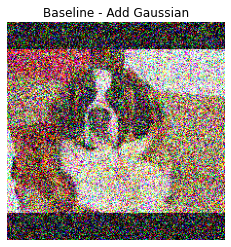
\includegraphics[width=\textwidth]{methods/images/ig-saint_bernard-gaussian.png}
    \caption{Gaussian Baseline}\label{fig:ig-baseline-gaussian}
\end{subfigure}
 \begin{subfigure}{.23\textwidth}
    \centering
    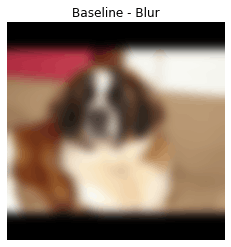
\includegraphics[width=\textwidth]{methods/images/ig-saint_bernard-blur.png}
    \caption{Blur Baseline}\label{fig:ig-baseline-blur}
\end{subfigure}
 \begin{subfigure}{.23\textwidth}
    \centering
    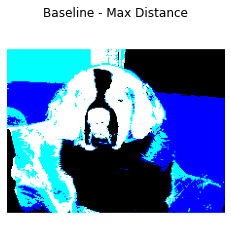
\includegraphics[width=\textwidth]{methods/images/ig-saint_bernard-max-dist.png}
    \caption{Max Distance Baseline}\label{fig:ig-baseline-max-dist}
\end{subfigure}
 \begin{subfigure}{.23\textwidth}
    \centering
    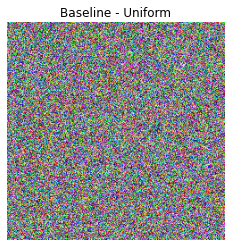
\includegraphics[width=\textwidth]{methods/images/ig-saint_bernard-uniform.png}
    \caption{Uniform Baseline}\label{fig:ig-baseline-uniform}
\end{subfigure}

 \caption{Alternative baselines for IG. Gaussian baseline is using $\sigma = 0.5$ to generate noise. Blur baseline is using $\sigma = 5$ in a gaussian filter. All the values are clipped at $<0,1>$ to be within the range of the scaled colors. Image source: \textit{Stanford Dogs} \cite{stanford-dogs} }\label{fig:ig-alternative baselines}
\end{figure}
\section{Guided GradCAM}

Guided GradCAM is a method created by Selvaraju et al. \cite{selvaraju2017grad} which combines both GBP and GradCAM (also created by the same authors). To explain the idea of Guided GradCAM, we have to split it into separate components.

\vspace{\baselineskip}

\textbf{Class Activation Mapping} (CAM) \cite{zhou2016learning} is an approach to localize regions responsible for a class prediction. This idea replaces the fully connected layers on the CNN with more convolutional layers and global average pooling (GAP) \cite{lin2013network}. 

\begin{figure}[h]
    \centering
    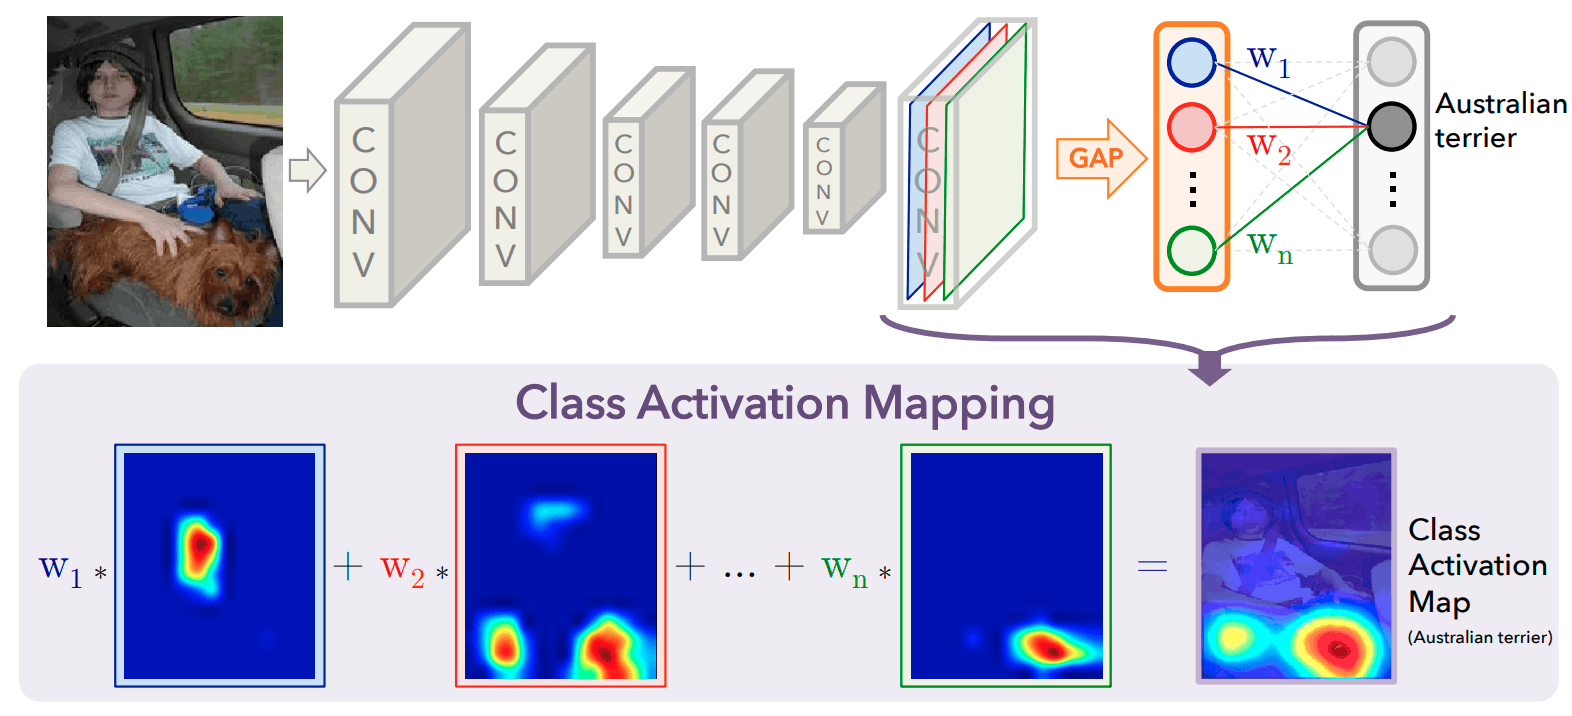
\includegraphics[width=\textwidth]{methods/images/cam-structure.png}
 \caption{The modified architecture of the CNN that produces CAMs. Source: \textit{Learning Deep Features for Discriminative Localization} \cite{lin2013network} }\label{fig:gradcam-cam}
\end{figure}

As shown in Figure \ref{fig:gradcam-cam}, just before the Softmax layer, the GAP operation is performed. This computes the spatial average of the feature map from the last CNN layer for every unit. The weighted sum of these spatial averages is calculated to produce the final output, and the Softmax layer gives us a normalized output used for classification. Class activation maps are computed similarly to the output, but the process is reversed. As an input, we have a class $c$, and the activation map for that class can be computed as:

\begin{equation}
    M_c(x,y) = \sum_{k=1}^{n} w_k^c f_k(x,y)
    \label{eq:cam-activation}
\end{equation}

Where $w_k^c$ is a weight corresponding to the unit $k$ and class $c$, and $f_k(x,y)$ is an activation of the last convolutional layer at the location $(x,y)$ for unit $k$ (visualized in Fig. \ref{fig:gradcam-cam}, the bottom part of the image).

\vspace{\baselineskip}

Selvaraju et al. argue that the CAM approach has a major drawback which is a requirement to modify the network and replace all fully-connected layers with convolutional layers. This makes CAM only applicable to certain tasks and reduces the performance of the network itself. They introduce the method that fixes all mentioned issues and call it \textbf{GradCAM}. This method is implementation agnostic (within the CNNs) and can be applied without any modifications to the network. As the name says, GradCAM uses a gradient to generate CAMs. Unlike in the original CAM paper, GradCAM allows selecting the convolutional layer we use as a feature map against which we compute the gradient. The gradient is computed for a given score $y^c$ ($c$ indicated a class) before the softmax layer. Then we use a feature map from the selected layer and calculate weight $a_k^c$ for every neuron (eq. \ref{eq:gradcam-weights}) (similar to calculating weight for every unit in CAM).

\begin{equation}
    a_k^c = \frac{1}{Z} \sum_{i} \sum_{j} \frac{\partial y^c}{\partial A_{ij}^k}
    \label{eq:gradcam-weights}
\end{equation}

\begin{figure}[ht]
    \centering
    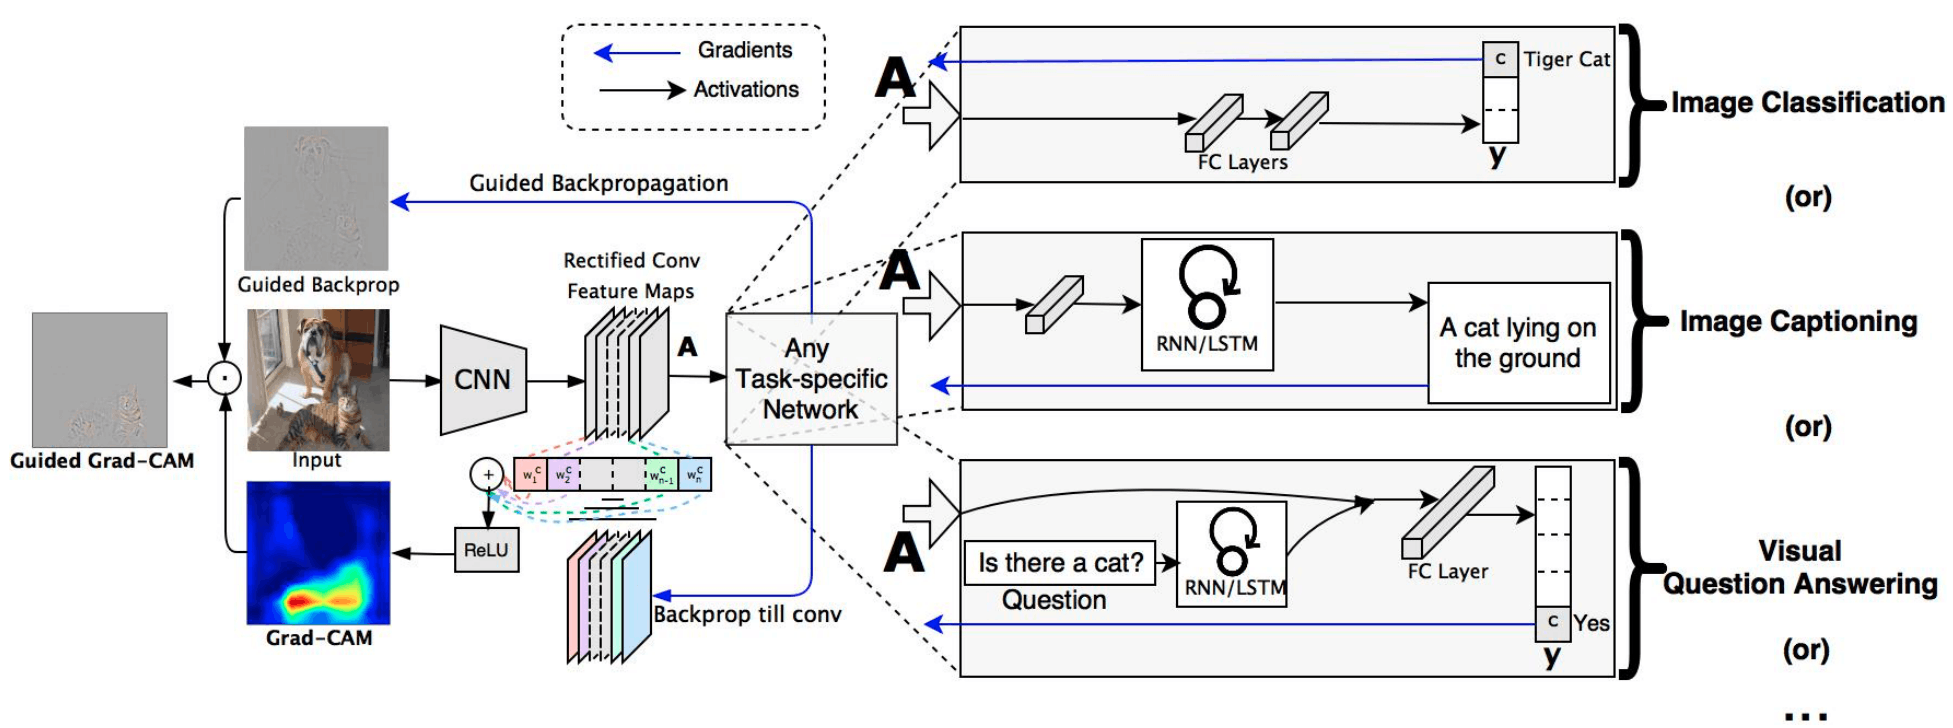
\includegraphics[width=\textwidth]{methods/images/guided-gradcam.png}
 \caption{Guided GradCAM computation process. Source: \textit{Grad-CAM: Visual Explanations from Deep Networks via Gradient-based Localization} \cite{selvaraju2017grad} }\label{fig:gradcam-guided-gradcam}
\end{figure}

$\frac{1}{Z} \sum_{i} \sum_{j}$ defines a global average pooling over the width ($i$) and height ($j$) and $\frac{\partial y^c}{\partial A_{ij}^k}$ is the gradient of score with respect to selected layers' feature map. With all $a_k^c$ calculated, we can perform a linear combination of feature maps $A^k$ and the neuron importance weights $a_k^c$ (eq. \ref{eq:gradcam-linear-combination}).

\begin{equation}
    M^c_{\text{GradCAM}} = \text{ReLU} \left(\sum_{k} a_k^c A^k \right)
    \label{eq:gradcam-linear-combination}
\end{equation}

The ReLU is used there to cutoff any non-positive values. The intuition behind using ReLU is that negative values more likely belong to other classes, which are also present in the image. The size of the map $M^c_{\text{GradCAM}}$ is the same as the size of the convolutional feature map used to compute the gradient. Values from the map then have to be mapped on the original image to visualize which region was relevant in predicting class $c$.

\begin{wrapfigure}{L}{0.50\textwidth}
  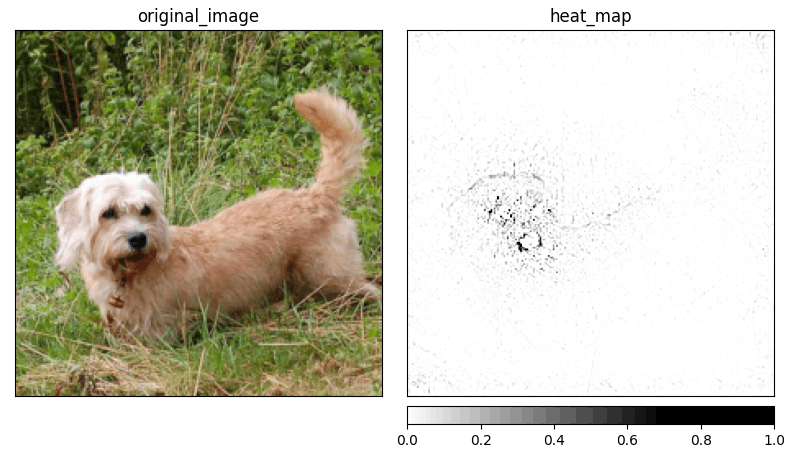
\includegraphics[width=0.50\textwidth]{methods/images/501-Dandie_Dinmont-Dandie_Dinmont.png}
  \caption{Visualization of the saliency map by the Guided GradCAM generated for the class \textit{dandie\_dinmont}. Image source: \textit{Stanford Dogs} \cite{stanford-dogs}}\label{fig:gradcam-dandie}
\end{wrapfigure}

\vspace{\baselineskip}

Guided GradCAM is a combination of GradCAM's map and GBP attribution. To compute the Guided GradCAM value, we are performing Hadamard product (also known as element-wise multiplication) of the attribution from GBP with a map from GradCAM (see Fig. \ref{fig:gradcam-guided-gradcam}). Combining GBP and GradCAM allow us to generate sharp attributions, as presented in Figure \ref{fig:gradcam-dandie}.
\section{Gradient SHAP}

Gradient SHAP (GradSHAP) was introduced by Erion et al. \cite{erion2019learning}\footnote{This paper is a preprint, it is still under the review at ICLR conference} and combined ideas from Integrated Gradients \cite{sundararajan2017axiomatic}, SHAP \cite{lundberg2017unified}, and SmoothGrad \cite{smilkov2017smoothgrad}. As mentioned in chapter \ref{section:ig}, IG has a problem with selecting the right baseline for specific a model. There were attempts to fix a problem with the baseline \cite{smilkov2017smoothgrad}\cite{fong2017interpretable}\cite{sturmfels2020visualizing} but selecting the right baseline with the "absence of feature" depends highly on the model architecture and datasets used in the training process.


\begin{equation}
    ExpectedGradients_{i}(x) ::= \int_{x'}\left( (x_{i} - x'_{i})\times\int_{\alpha=0}^1\frac{\partial F(x'+\alpha \times (x - x'))}{\partial x_i}{d\alpha} \right)p_D(x')\partial x'
    \label{eq:gradshap-full-eq}
\end{equation}

Erion et al. present an idea of \textit{expected gradients}, which tries to avoid specifying single $x'$ and use the data distribution instead $p_D$ (eq. \ref{eq:gradshap-full-eq}). Where $x$ is an input vector, $F$ is a model, $\alpha$ is an interpolation factor.


\begin{equation}
    ExpectedGradient^{expected}_{i}(x) ::= \underset{x' \sim D, \alpha \sim U(0,1)}{E} \left[(x_{i}-x'_{i})\times\frac{\partial F(x'+\alpha \times (x - x'))}{\partial x_i} \right]
    \label{eq:gradshap-aprox}
\end{equation}

As in the IG definition (eq. \ref{eq:ig-full-eq}), calculating the integral is not possible, two integrals in the Expected Gradients have the approximate value solution (eq. \ref{eq:gradshap-aprox}). Where $D$ is a our data and $\alpha$ comes from the uniform distribution $U(0,1)$.

\begin{wrapfigure}{L}{0.40\textwidth}
  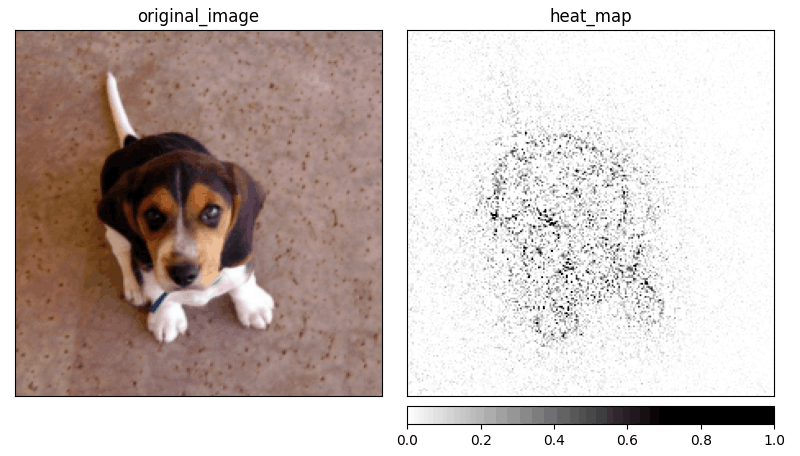
\includegraphics[width=0.40\textwidth]{methods/images/gradshap-beagle.png}
  \caption{Visualization of the saliency map by the GradSHAP generated for the class \textit{beagle}. The result is calculated with five random samples. Image source: \textit{Stanford Dogs} \cite{stanford-dogs}}\label{fig:gradshap-beagle}
  \vspace{1mm}
\end{wrapfigure}

In practice, this approach allows to approximate SHAP values. It computes expectations of gradients by sampling from the baselines and add noise to each input sample, $n$ times. GradSHAP assumes that input features are independent of each other and the explanation is simply a composition of individual features' contribution.

\vspace{\baselineskip}

In recent implementations \cite{kokhlikyan2020captum}, the method has multiple variants. One of the most important changes is to allow to replace $U(0,1)$ with the Gaussian distribution ${\mathcal {N}}(0 ,\sigma ^{2})$. Using a Gaussian distribution allows modifying the standard deviation $\sigma$ base on the original data. An example of the attribution generated by the GradSHAP method is shown in Figure \ref{fig:gradshap-beagle}.
\section{Noise Tunnel}

Noise Tunnel \cite{kokhlikyan2020captum} is not an attribution method but a technique that improves the accuracy of attribution methods. It combines SmoothGrad \cite{smilkov2017smoothgrad}, SmoothGrad-Square (unpublished version of the SmoothGrad), and VarGrad \cite{adebayo2018sanity} and works with most of the attribution methods.

\vspace{\baselineskip}

Noise Tunnel addresses a problem described in sections \ref{section:gbp} and \ref{section:ig}, where we discussed the problem with \textit{ReLU} activation function and gradients producing noisy, often irrelevant attributions. Because the partial derivative $\frac{\partial F_c}{\partial x_i}$ of the models' score $F_c$ for a class $c$ with respect to the value of the pixel $x_i$ fluctuates, Smilkov et al. \cite{smilkov2017smoothgrad} thought that adding a Gaussian noise ${\mathcal {N}}(0, 0.01^2)$ and calculating an average of sampled attributions is going to solve the problem.

\begin{equation}
\hat{M}_{c}(x)=\frac{1}{n} \sum_{1}^{n} M_{c}\left(x+\mathcal{N}\left(0, \sigma^{2}\right)\right)
\label{eq:smoothgrad}
\end{equation}

SmoothGrad (eq. \ref{eq:smoothgrad}) calculates the attribution ($M_c$) using any available method by providing that method an input with Gaussian noise. It then calculates a mean value from all the samples to reduce the importance of less frequent attributions. The idea is that when adding noise to the input image, important attributions are going to be visible most of the time, and noise might change between attributions.

\vspace{\baselineskip}

Another version of the SmoothGrad Noise Tunnel is SmoothGrad-Square. It changes only the way that the mean value is calculated by using the mean of squared attributions instead of just attributions (eq. \ref{eq:smoothgrad-sq}). This method usually provides less noisy results (compare Fig. \ref{fig:noisetunnel-smoothgrad-dingo} and Fig. \ref{fig:noisetunnel-smoothgrad-sq-dingo}) but often removes less important features, which are still valid features.

\begin{equation}
\hat{M}_{c}(x)=\frac{1}{n} \sum_{1}^{n} \sqrt{M_{c}\left(x+\mathcal{N}\left(0, \sigma^{2}\right)\right)}
\label{eq:smoothgrad-sq}
\end{equation}

The third version of Noise Tunnel is a version using VarGrad (see Fig. \ref{fig:noisetunnel-vargrad-dingo}) which is a variance version of the SmoothGrad and can be defined as Eq. \ref{eq:vargrad}, where $\hat{M}_c$ is a value of SmoothGrad. 

\begin{equation}
\tilde{M}_{c}(x)=\frac{1}{n} \sum_{k=1}^{n}\left\{M_{c}\left(x+\mathcal{N}\left(0, \sigma^{2}\right)\right)\right\}^{2}-\left\{\hat{M}_{c}(x)\right\}^{2}
\label{eq:vargrad}
\end{equation}

\begin{figure}[h]
  \centering
 \begin{subfigure}{.19\textwidth}
    \centering
    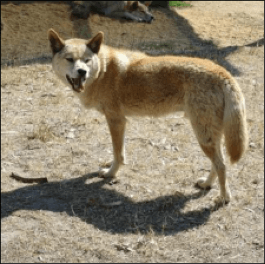
\includegraphics[width=\textwidth]{methods/images/dingo.png}
    \caption{Original image}\label{fig:noisetunnel-dingo}
\end{subfigure}
 \begin{subfigure}{.19\textwidth}
    \centering
    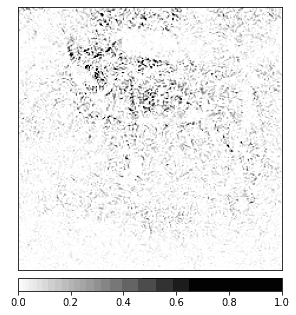
\includegraphics[width=\textwidth]{methods/images/ig-dingo.png}
    \caption{IG}\label{fig:noisetunnel-ig-dingo}
\end{subfigure}
 \begin{subfigure}{.19\textwidth}
    \centering
    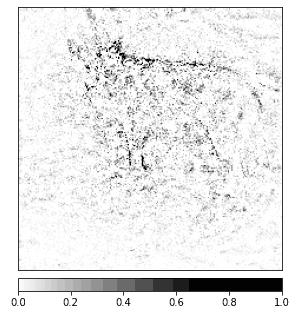
\includegraphics[width=\textwidth]{methods/images/ig-smoothgrad-dingo.png}
    \caption{SmoothGrad}\label{fig:noisetunnel-smoothgrad-dingo}
\end{subfigure}
 \begin{subfigure}{.19\textwidth}
    \centering
    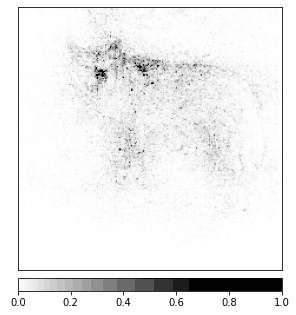
\includegraphics[width=\textwidth]{methods/images/ig-smoothgrad-sq-dingo.png}
    \caption{SmoothGrad-Sq}\label{fig:noisetunnel-smoothgrad-sq-dingo}
\end{subfigure}
 \begin{subfigure}{.19\textwidth}
    \centering
    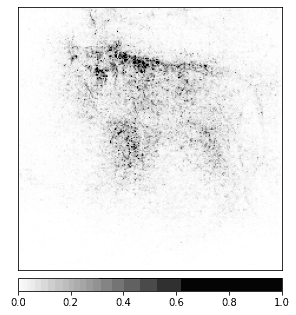
\includegraphics[width=\textwidth]{methods/images/ig-vargrad-dingo.png}
    \caption{VarGrad}\label{fig:noisetunnel-vargrad-dingo}
\end{subfigure}

 \caption{Visualisation of saliency maps produced by \textit{IG} (\ref{fig:noisetunnel-ig-dingo}), \textit{IG with SmoothGrad} (\ref{fig:noisetunnel-smoothgrad-dingo}), \textit{IG with SmoothGrad-Square} (\ref{fig:noisetunnel-smoothgrad-sq-dingo}), and \textit{IG with VarGrad} (\ref{fig:noisetunnel-vargrad-dingo}) of the same input image \ref{fig:noisetunnel-dingo} for a class \textit{dingo}. All the maps are generated using the same model (ResNet18). All noise tunnels are generating 10 random samples from ${\mathcal {N}}(0,1)$ distribution. Image source: \textit{Stanford Dogs} \cite{stanford-dogs} }\label{fig:noisetunnel-comparison-dingo}
\end{figure}

When comparing all the methods used in Noise Tunnel, we can see major differences in comparison with the original attribution (see Fig. \ref{fig:noisetunnel-comparison-dingo}). Using SmoothGrad (Fig. \ref{fig:noisetunnel-smoothgrad-dingo}) seams to detect more edges of the input image (in comparison with pure IG attribution in Fig. \ref{fig:noisetunnel-ig-dingo}), and that can be interpreted as detecting decision boundary. SmoothGrad-Square (Fig. \ref{fig:noisetunnel-smoothgrad-sq-dingo}) and VarGrad (Fig. \ref{fig:noisetunnel-vargrad-dingo}) are removing a large amount of noise but usually also some of the important features visible on the attribution from SmoothGrad (look on the tail of the dingo). In my work, if referring to Noise Tunnel, the default option will be the SmoothGrad version (unless specified otherwise).

\chapter{Measures}\label{chapter:measures}
\thispagestyle{chapterBeginStyle}

\vspace{-20mm}
\section{Sensitivity}\label{section:sensitivity}

Sensitivity \cite{yeh2019fidelity} (\textit{max-sensitivity} to be precise) is defined as a measure of change in the attribution with a small perturbation to the input.


\begin{definition}[Sensitivity]\label{def:sensitivity}
    For a given model $F$, attribution method $\Phi$, input $x$, insignificant perturbation $\delta$, and input neighborhood radious $r$, \textit{max-sensitifity} for a attribution is defined as:
    
    \begin{equation}
        \operatorname{SENS}_{\operatorname{MAX}}(\Phi, \mathbf{F}, \mathbf{x}, r):=\max _{\|\mathbf{\delta}\| \leqslant r} \| \Phi(\mathbf{F}, \mathbf{x} + \mathbf{\delta})-\Phi(\mathbf{F}, \mathbf{x}) \|
        \label{eq:sensitivity}
    \end{equation}
\end{definition}

\begin{wrapfigure}{L}{0.35\textwidth}
  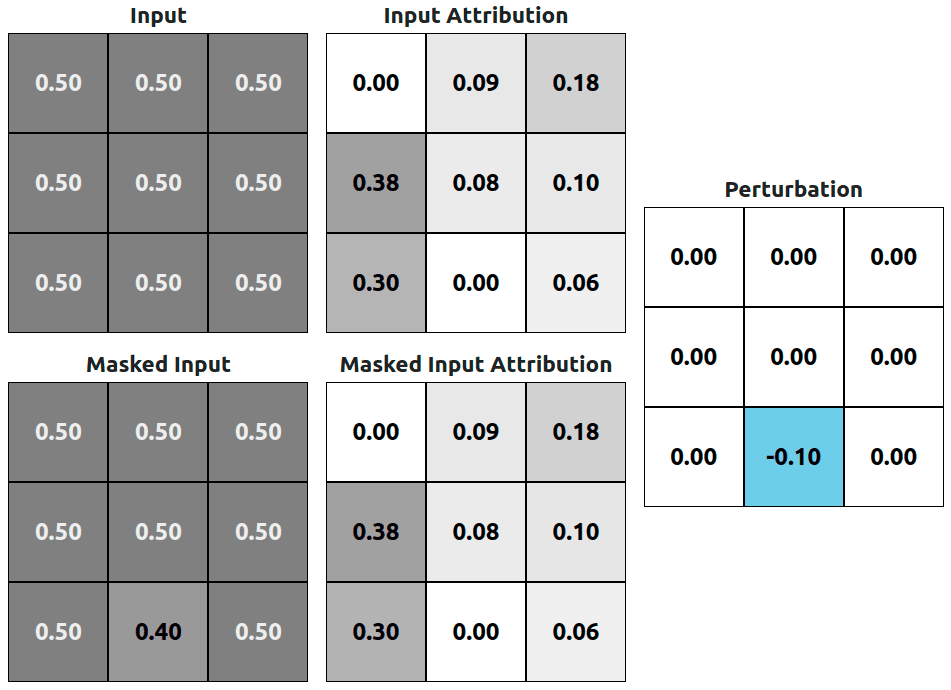
\includegraphics[width=0.35\textwidth]{methods/images/same-sens.png}
  \caption{\textbf{Sensitivity = 0}. Perturbation of the input did not change the attribution between the input and masked input (one with added perturbation).}\label{fig:sensitivyt-same}
  \smallskip\par
  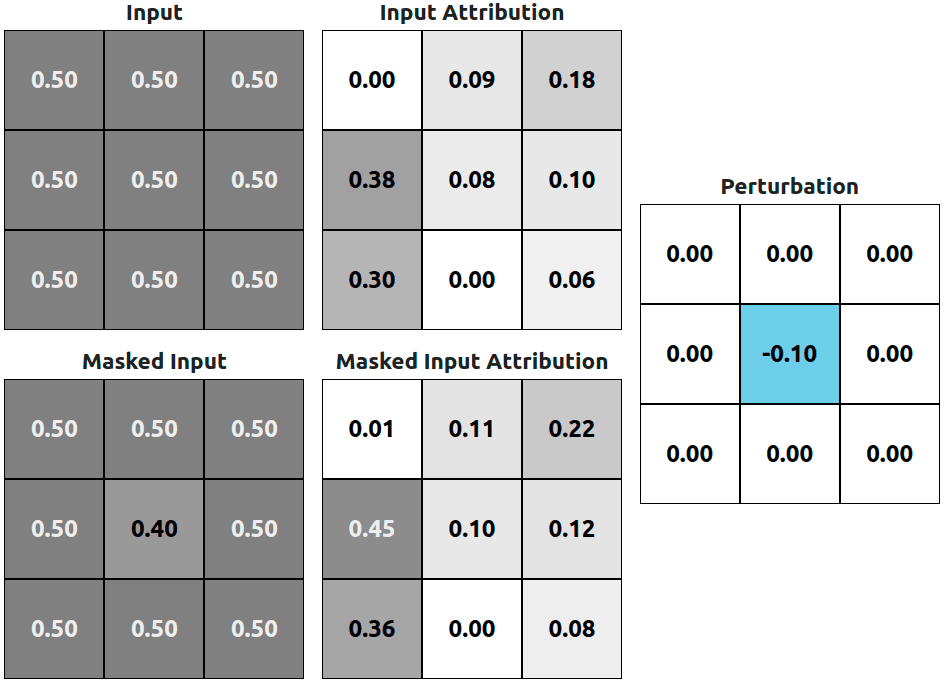
\includegraphics[width=0.35\textwidth]{methods/images/change-sens.png}
  \caption{\textbf{Sensitivity = 0.11}. Perturbation of the feature with higher than zero initial attribution causes Sensitivity value to rise.}\label{fig:sensitivyt-change}
\end{wrapfigure}


The radius $r$ serves as a radius of a $l_p norm$ used to generate insignificant perturbation. It restricts the range of the perturbation and usually is set to around $0.02$. Sensitivity returns a positive scalar which is the length of the sensitivity vector. This vector (as shown in eq. \ref{eq:sensitivity}) is the difference between two attribution vectors, so the absolute length of this vector is proportional to the difference in every dimension of the attribution vectors.



\vspace{2\baselineskip}

To explain the intuition behind the sensitivity, we can use a toy example of the model that takes $3x3$ input and predicts the class $[0,1]$. This model predicts class $0$ with a $0.95$ score when receiving the input filled with $0.50$. Attribution for this prediction is shown in Figure \ref{fig:sensitivyt-same} (Input Attribution). If a perturbation is added to the input, then new attribution is calculated for the same class ($0$) but for the \textit{Masked Input}. If the perturbation doesn't affect the attribution (as in Fig. \ref{fig:sensitivyt-same}), then returned Sensitivity measure is equal to zero.

\vspace{\baselineskip}

It is common for attribution to remain constant when perturbing features of the input with initial attribution close to zero. Attribution defines how much specific feature is involved in the model decision. Changing the value, which is irrelevant for the model, usually results in close to no change in the attribution.

\vspace{\baselineskip}

An example that causes the $\operatorname{SENS}$ value to change can be seen in Figure \ref{fig:sensitivyt-change}. This time perturbation changes the feature with non-zero attribution of the original input (\textit{Input Attribution}). That perturbation causes the new attribution (\textit{Masked Input Attribution}) to differ slightly from the original one. The length of the vector (total difference between two attributions) is equal to $0.11$ which is a square root of squared differences between corresponding attribution positions.

\vspace{\baselineskip}

\textbf{Remark.} Perturbation shown in the example is created for the purpose of the example. In practice, values in the perturbation will be significantly smaller and will affect the whole input, not only one feature.
\section{Infidelity}\label{section:infidelity}

Infidelity \cite{yeh2019fidelity} comes from the idea of fidelity, which could be defined as the amount of how many features with high attributions belong to a priori subset of features that are relevant to the prediction. This definition assumes that we have such a subset of relevant features, and that is not a valid assumption in most situations. In another paper \cite{ancona2017towards}, Ancona et al. are trying to come up with a quantitative measure for the XAI methods, which has no human bias. The idea is to relate the new measure to the correlation between the importance of features and the change in models' prediction. This can be achieved by perturbing the input and calculating the correlation between the perturbation of features with the predicted score.

\begin{definition}[Infidelity]\label{def:infidelity}
    For a given model $F$, attribution method $\Phi$, input $x$, and significant perturbation around input $I$, \textit{infidelity} for an attribution method is defined as:
    
    \begin{equation}
        \operatorname{INFD}(\Phi, \mathbf{F}, \mathbf{x})=\mathbb{E}_{\mathbf{I} \sim \mu_{\mathrm{I}}}\left[\left(\mathbf{I}^{T} \Phi(\mathbf{F}, \mathbf{x})-(\mathbf{F}(\mathbf{x})-\mathbf{F}(\mathbf{x}-\mathbf{I}))\right)^{2}\right]
        \label{eq:infidelity}
    \end{equation}

\end{definition}

Infidelity measure (eq. \ref{eq:infidelity}) consists of two major part which expected difference is a measure of infidelity. The first part ($\mathbf{I}^{T} \Phi(\mathbf{F}, \mathbf{x})$) is a dot product between the perturbation and the attribution generated by the XAI method. Attribution used for the calculation is the attribution for the image without perturbation. This method does not rely on the attribution of the perturbed image anywhere. The second part $(\mathbf{F}(\mathbf{x})-\mathbf{F}(\mathbf{x}-\mathbf{I}))^{2}$ is a squared difference between the score of the original image and the perturbed image. The perturbation is usually drawn from the Gaussian distribution with the $\mu = 0$, and the $\sigma$ is the parameter.

\begin{wrapfigure}{L}{0.40\textwidth}
  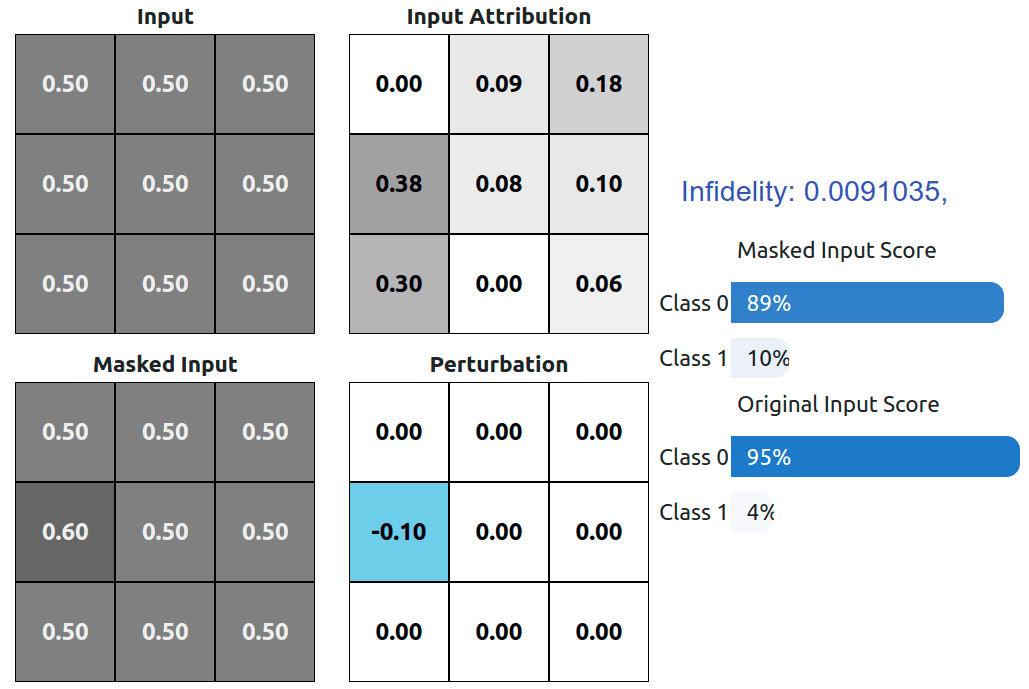
\includegraphics[width=0.40\textwidth]{methods/images/infidelity-small.png}
  \caption{Small perturbation of the feature value with the high initial attribution results in a small infidelity measure.}\label{fig:infidelity-small}
  \smallskip\par
  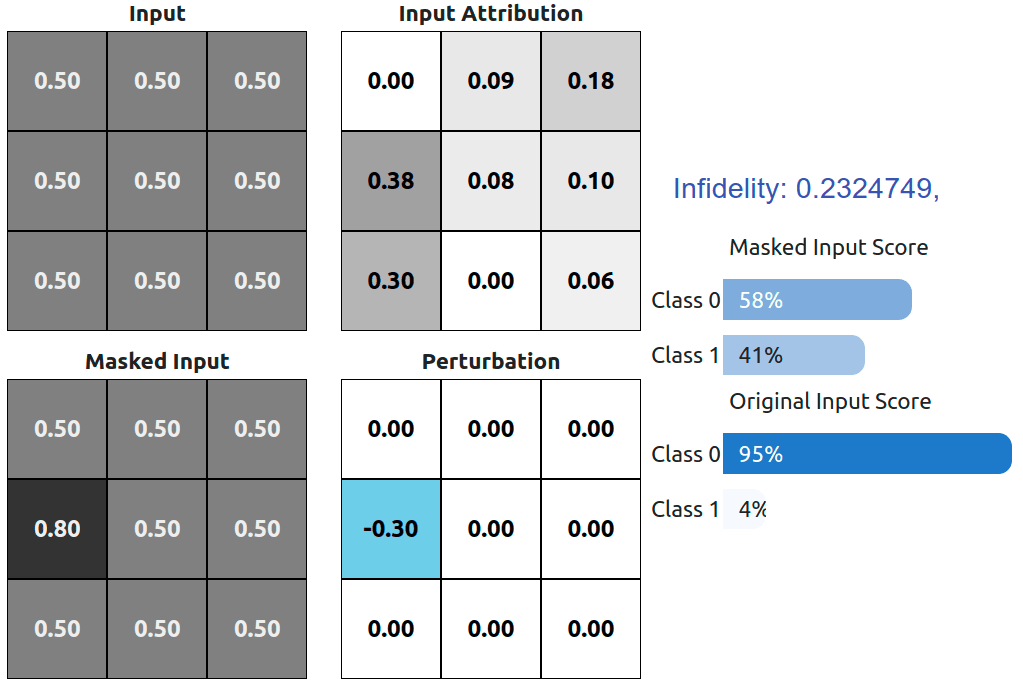
\includegraphics[width=0.40\textwidth]{methods/images/infidelity-large.png}
  \caption{High perturbation of the feature value with the high initial attribution results in a large infidelity measure.}\label{fig:infidelity-large}
\end{wrapfigure}

\vspace{\baselineskip}

To explain the intuition behind the infidelity measure as mentioned in section \ref{section:sensitivity}. This time the perturbation is done on the feature with high initial attribution of $0.38$. The first part of the equation is a dot product between transposed \textit{Perturbation} matrix and the \textit{Input Attribution} matrix. The second part is a difference between the \textit{Original Input Score} of class $0$ and the \textit{Masked Input Score} of class $0$.

\vspace{\baselineskip}

As shown in Figure \ref{fig:infidelity-small}, changing the feature with high attribution by a small amount ($-0.1$) resulted in a relatively small infidelity score of $0.0091$. This value is primarily due to a small change in the class prediction between input and the masked input. The next example (Fig. \ref{fig:infidelity-large}) shows a significantly larger value of infidelity. This time the change in score is greater in relation to change in the input features (score for class $0$ dropped by $0.37$ for $0.3$ change in the value of the feature). 

\vspace{\baselineskip}

These two examples show how infidelity behaves and what it tries to measure. If the initial attribution of the feature is correct, then the infidelity values should be close to zero. If the correlation between attribution value and the change in models' prediction varies, then the infidelity values should be higher. By definition, the measure checks if the fidelity of the attributions relates to what the model predicts.
\section{RemOve And Retrain}\label{section:roar}

The ROAR (RemOve And Retrain) framework \cite{hooker2018benchmark} is another approach to compare XAI methods. The assumption is that if the feature attribution is correct, then by removing those features, the classifies should degrade. This assumption is based on the work done by Samek et al.\cite{samek2016evaluating} and shows promising results. Hooker argues that the method violates the key assumption of machine learning, where the training data and the test data have to be from the same distribution. By removing attributed features, we are creating data samples that come from different distribution, and therefore loss in the classification performance might be due to the distribution shift. To solve that problem, the authors propose to retrain the model on the dataset with removed features and then compare the models' performance.

\begin{figure}[ht]
    \centering
    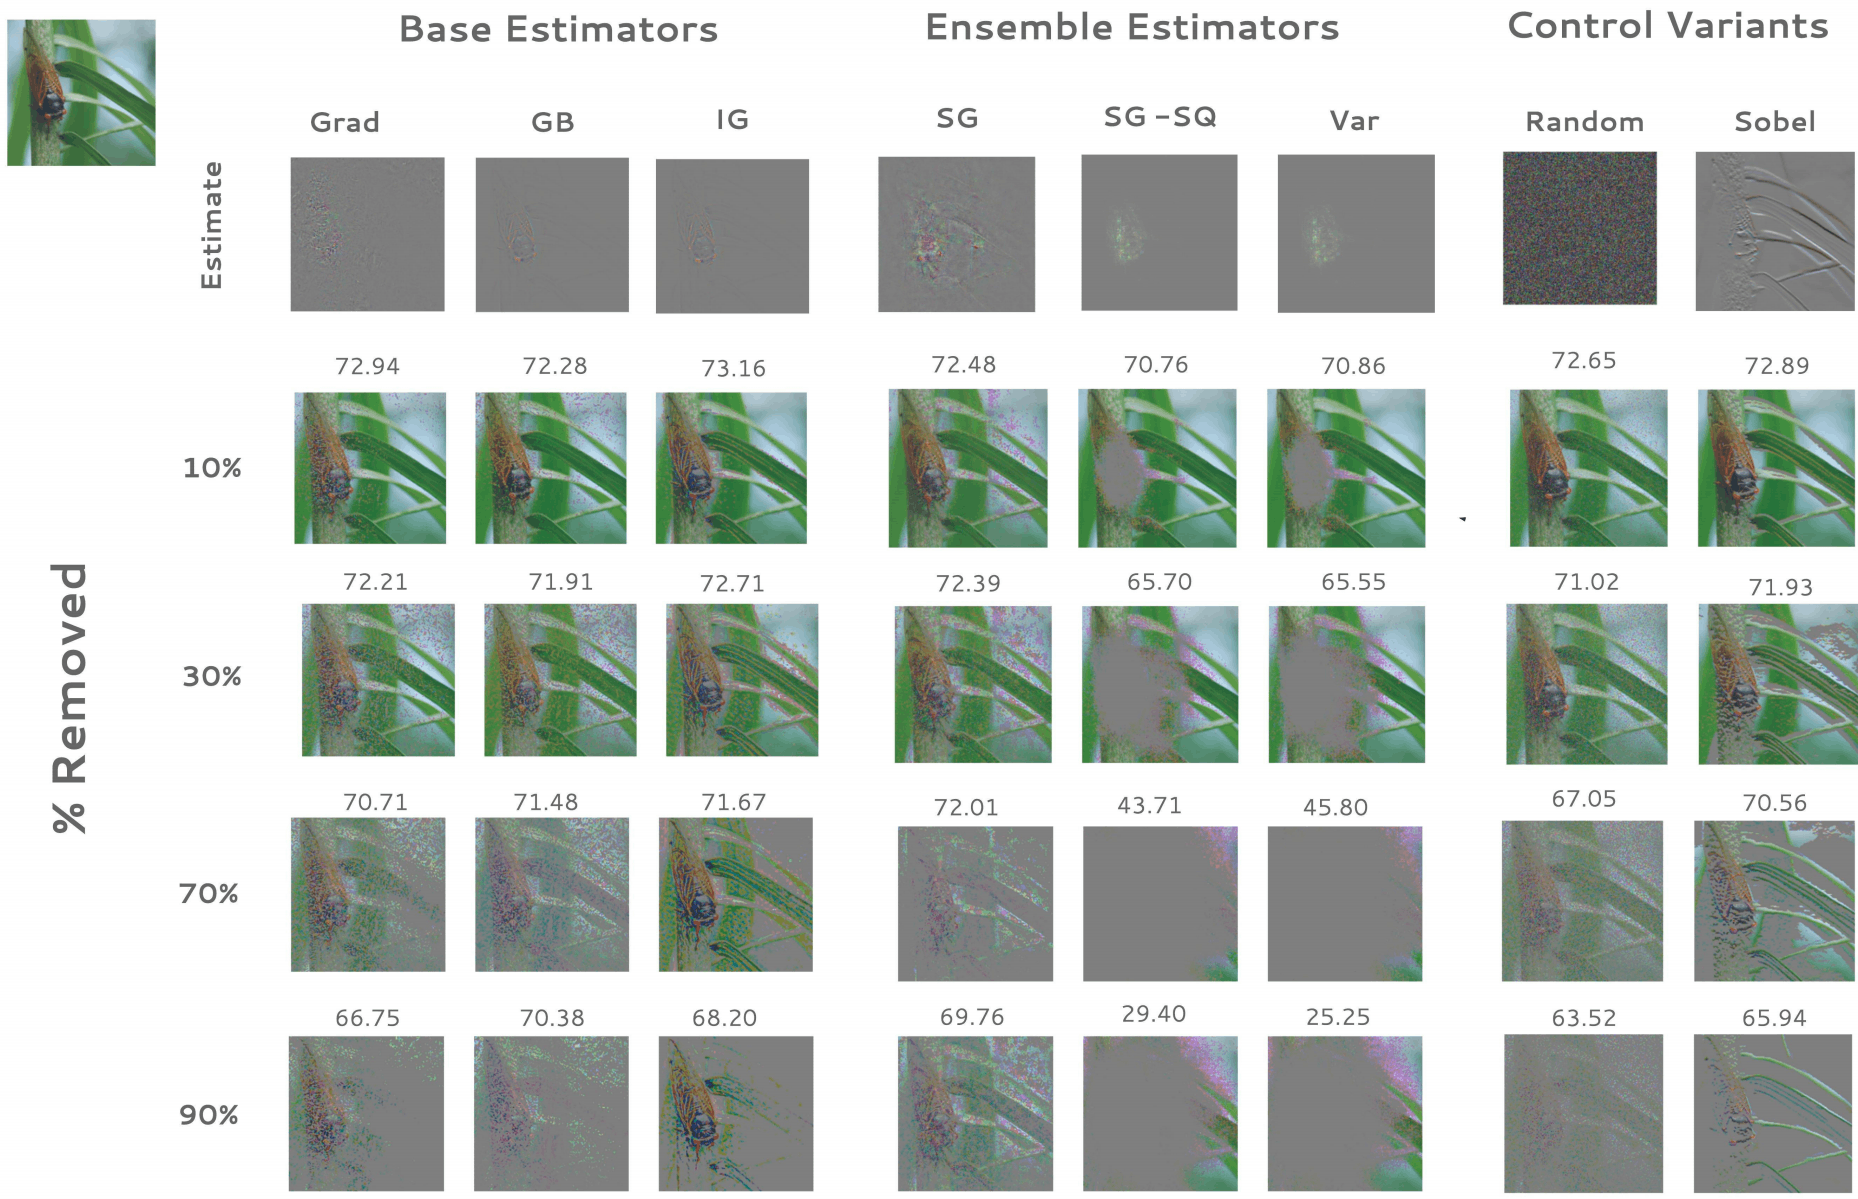
\includegraphics[width=\textwidth]{methods/images/roar-remove.png}
 \caption{Modification of the image according to the ROAR framework. The percentage of the pixels with the highest attributions is replaced by the mean value (\textit{\% Removed}). Scores above each image refer to the average test accuracy of the models trained on modified dataset. Methods used in the experiments: Saliency (GRAD) \cite{simonyan2014deep}, Guided Backpropagation (GPB) \cite{springenberg2014striving}, Integrated Gradients (IG) \cite{sundararajan2017axiomatic}, SmoothGrad (SG) and SmoothGrad-Square (SG-SQ) \cite{simonyan2014deep}, VarGrad (Var) \cite{selvaraju2017grad}, Random Bernoulli, Sobel Edge Filter. Source: \textit{A Benchmark for Interpretability Methods in Deep Neural Networks} \cite{hooker2018benchmark} }\label{fig:roar-remove}
\end{figure}

For the framework to work, it has to generate input attribution for the image and order each feature attribution from the most important to the less important. With the ordered list, it can remove a given top $t\%$ of features and replace them with a mean value of all pixels (see Fig. \ref{fig:roar-remove}). This process is repeated for $t = [0, 10, ..., 100]$ ($t$ is a percentage of all features). After removing those features, a new model is trained on the modified dataset, and the degradation in accuracy is calculated.

\begin{figure}[ht]
    \centering
    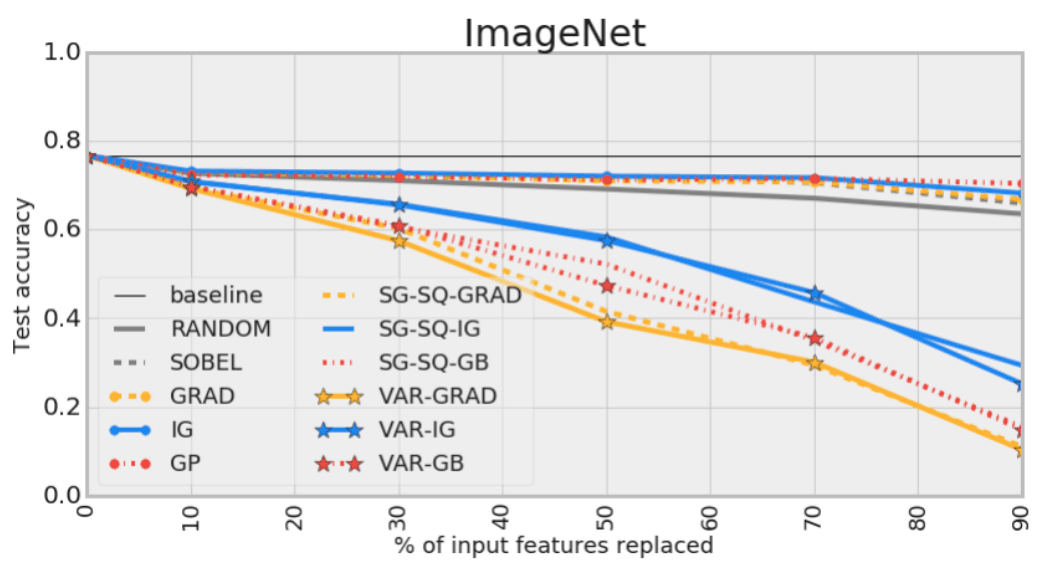
\includegraphics[width=\textwidth]{methods/images/roar-results.png}
 \caption{Results from the ROAR framework on the ImageNet dataset \cite{russakovsky2015imagenet}. A method with the highest drop (Saliency-based Noise Tunnel with VarGrad) is considered to be the one with the most relevant attribution. The biggest drop in the accuracy, the better the XAI method is according to the assumptions. Source: \textit{A Benchmark for Interpretability Methods in Deep Neural Networks} \cite{hooker2018benchmark} }\label{fig:roar-results}
\end{figure}

As shown in Figure \ref{fig:roar-results}, methods using Noise Tunnel achieve significantly better results from their original versions. The ROAR framework with its approach to compare XAI methods is an interesting proposition but has one important drawback. Every time the method is tested, we have to retrain hundreds of models, and without a computation cluster, this is not possible in an acceptable time frame.
\section{Structural Similarity Index Measure}

Structural Similarity Index Measure (SSIM) \cite{wang2004image} is a metric used to calculate the similarity between two images. It measures a perceived change in the structural information between images and is used for picture comparison in television. The index does not use the whole image but rather $NxN$ windows to calculate similarity scores. The window size used in the original paper is $11x11$, and if not specified otherwise, this is a window used in my work. The SSIM is defined as:

\begin{equation}
    {\displaystyle {\hbox{SSIM}}(x,y)={\frac {(2\mu _{x}\mu _{y}+(k_1L)^2)(2\sigma _{xy}+(k_2L)^2)}{(\mu _{x}^{2}+\mu _{y}^{2}+(k_1L)^2)(\sigma _{x}^{2}+\sigma _{y}^{2}+(k_2L)^2)}}}
    \label{eq:ssim}
\end{equation}

Where $x$ and $y$ are the images to compare, $mu _{x}$ and $mu _{y}$ are the mean values of pixels from the window. $\sigma _{x}$ and $\sigma _{y}$ are the variance of those pixels from the window, and $\sigma _{xy}$ is a covariance of $x$ and $y$. There is also the $L$ parameter, which is important when trying to compare SSIM values calculated for the images from different distributions. This parameter defined a dynamic range of values present in the image. In the case of comparing attributions, it usually is a maximum value of attribution from a given dataset (assuming the same attribution method and model). Values of $k_1$ and $k_2$ are constant and equal to $0.01$ and $0.03$ accordingly.

\begin{figure}[h]
  \centering
 \begin{subfigure}{.3\textwidth}
    \centering
    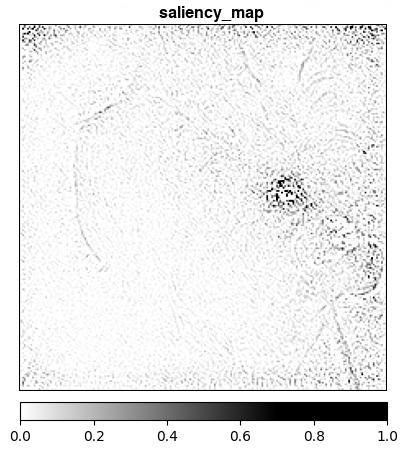
\includegraphics[width=\textwidth]{methods/images/cairn-none.jpg}
    \caption{Baseline}\label{fig:ssim-carin-none}
\end{subfigure}
 \begin{subfigure}{.3\textwidth}
    \centering
    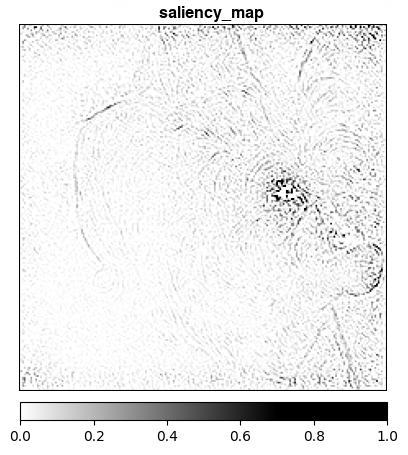
\includegraphics[width=\textwidth]{methods/images/cairn-sharp.jpg}
    \caption{$SSIM = 0.955$}\label{fig:ssim-carin-sharp}
\end{subfigure}
 \begin{subfigure}{.3\textwidth}
    \centering
    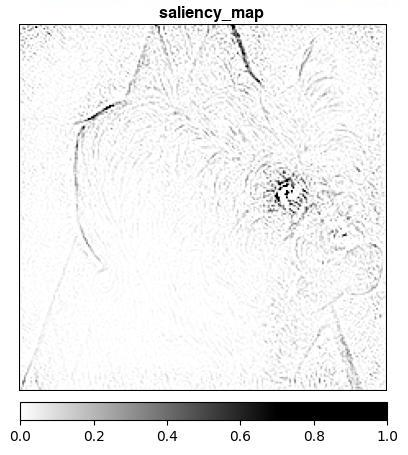
\includegraphics[width=\textwidth]{methods/images/cairn-norm.jpg}
    \caption{$SSIM = 0.885$}\label{fig:ssim-carin-norm}
\end{subfigure}

 \caption{SSIM scores for comparing the baseline attribution (Fig. \ref{fig:ssim-carin-none}) with attributions of augmented images. Image source: \textit{Stanford Dogs} \cite{stanford-dogs} }\label{fig:ssim-scores-example}
\end{figure}

The amount SSIM value change with the change in the perception of the image is presented in Figure \ref{fig:ssim-scores-example}. The higher score achieved when comparing image \ref{fig:ssim-carin-none} with \ref{fig:ssim-carin-sharp} can be related to the visual similarity between two images. We can clearly see that attribution from image \ref{fig:ssim-carin-norm} is sharper, and therefore less similar to the baseline.

\begin{remark}
Quantifying human visual perception is still an active field of research, and SSIM metric is not the perfect solution. There are other methods, but they all had some issues when compared with real humans. This metric is going to be used to qualitatively compare attributions because comparing thousands of images qualitatively is not possible in a reasonable amount of time.
\end{remark}
	\cleardoublepage
	
	\chapter{Experiments}\label{chapter:experiments}
\thispagestyle{chapterBeginStyle}

In this chapter, I will describe the experimental setup with all requires libraries. Section \ref{section:datasets} includes the description, analysis, and examples from the datasets used in the experiments. It also provides an explanation and the assumption on how to simulate a drop in the model performance \ref{remark:performance-drop-while-train} used in training. The model training process is defined in section \ref{section:models}. Because the model performance and training are not a part of experiments, training results are also added to this section. Real-world augmentations used in this study are defined in section \ref{section:augmentation}. These augmentations are applied to the images in the first part of the experiments (described in Section \ref{section:dont-augment-me-definition}). Experiments are divided into two parts. The first part (defined in Section \ref{section:dont-augment-me-definition}) is going to test the effect that augmentations have on attribution methods. The second part (defined in Section \ref{section:can-i-rely-on-you-definition}) is going to check if there is a reliable measurement that can be used to compare XAI methods.

\section*{Environment and framework}

The training environment was designed around the PyTorch library \cite{NEURIPS2019_9015}\footnote{Detailed implementation and guide is available at \url{https://github.com/burnpiro/xai-correlation}, Wiki page with additional instructions and results is available at \url{https://github.com/burnpiro/xai-correlation/wiki}}. Augmentations described in section \ref{section:augmentation} are performed with the help of the G'MIC library \cite{gmic}. Most of the experiments use Captum \cite{kokhlikyan2020captum} and scikit-learn \cite{scikit-learn} libraries to process, analyze and produce results of attribution methods. In the experiments, not all methods are used for all experiments. This is due to the limited amount of memory available on the graphic card used to perform analysis. Methods like Integrated Gradients \cite{sundararajan2017axiomatic} cannot be used to calculate the value of Sensitivity \cite{yeh2019fidelity} because it requires storing over $500$ interpolations to generate the result. These details will be explained in sections describing a particular experiment. All the experiments are run on the \textit{GeForce GTX 1080 Ti} with 11GB of memory, and the total processing time of all experiments is around 508 hours (this assumes running a version with example generation).

\section{Datasets}\label{section:datasets}

All the datasets used in this study are publicly available. The selection process was aimed at finding a variety of different domains and complexity. Five datasets were selected, and each dataset is split into a training dataset and test dataset. If not defined in the dataset description, the split was done using $80:20$ proportions (\textit{training : test}). Besides the original split, each training dataset was additionally split into five training datasets. The second split creates the following structure for every dataset:

\begin{table}[ht]
\centering
\caption{Default dataset split structure}
\label{tab:dataset-split}
\begin{tabular}{|l|l|l|}
\hline
  & Training     & Test \\ \hline
A & 100\% * 80\% & 20\% \\ \hline
B & 80\% * 80\%  & 20\% \\ \hline
C & 60\% * 80\%  & 20\% \\ \hline
D & 40\% * 80\%  & 20\% \\ \hline
E & 20\% * 80\%  & 20\% \\ \hline
\end{tabular}
\end{table}

Table \ref{tab:dataset-split} can be read as \textit{"split B of the dataset X uses 80\% training dataset which consists of 80\% of the entire dataset, and full test dataset which consists of 20\% of the total dataset"}. If the class distribution is not constant, then splits of the train datasets are stratified. 

\begin{remark}\label{remark:performance-drop-while-train}
This split assumes that using a fraction of the training dataset for training will cause models to perform worse when tested on the same test dataset. It should simulate real-world issues with model accuracy and allow to experiment on none perfect models. The drop in the accuracy is not going to be linear because of the different complexities of each data domain.
\end{remark}

\subsection{Stanford Dogs}

The dataset created by Stanford University consists of dog pictures. It has 120 classes, and the train/test data split is defined by the authors. Class distribution is proportional between train and test splits. Dataset is slightly unbalanced, with the ratio between the least frequently occurring class and the most common class being $1.7$ (detailed class distribution available in appendix \ref{appendix:datasets:stanford-dogs}). The total number of images is 20580 (train: 16418, test: 4162). Examples from the datasets can be seen in Figure \ref{fig:stanford-dogs-example}.

\begin{figure}[ht]
    \centering
    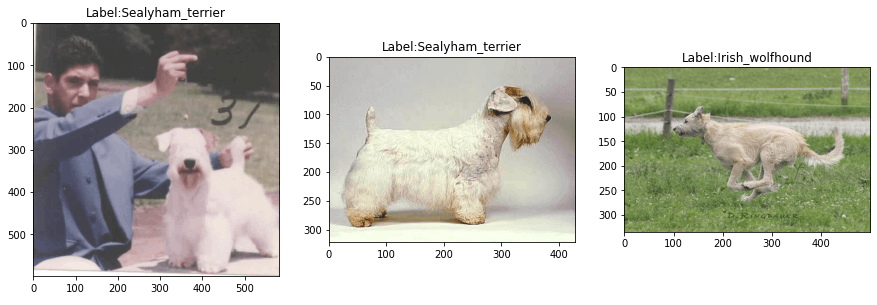
\includegraphics[width=0.65\textwidth]{experiments/datasets/dogs.png}
    \caption{Example images from in \textit{Stanford Dogs} \cite{stanford-dogs}}\label{fig:stanford-dogs-example}
\end{figure}

\subsection{Food 101}

The dataset consists of food pictures. It has 101 classes, and the train/test data split is defined by the authors. Classes are distributed proportionally, and each class has 750 examples in the train dataset and 250 examples in the test dataset, with the total number of images at 101000 (train: 75750, test: 25250). Examples from the datasets can be seen in Figure \ref{fig:food101-example}.

\begin{figure}[ht]
    \centering
    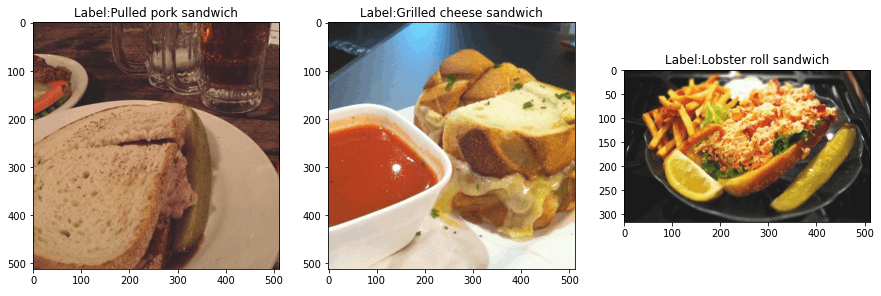
\includegraphics[width=0.65\textwidth]{experiments/datasets/food101.png}
    \caption{Example images from in \textit{Food 101} \cite{food101}}\label{fig:food101-example}
\end{figure}

\subsection{Edible wild plants}

The dataset consists of edible wild plants pictures. It has 62 classes, and the train/test data split is defined by the authors. Class distribution differs between train and test splits. Train dataset is highly unbalanced, with the ratio between the least frequently occurring class and the most common class being $21$ (detailed class distribution available in appendix \ref{appendix:datasets:edible-plants}). The unbalance is caused by 3 major classes. The rest of the dataset has the same ratio equal to $3$. The test dataset is balanced with $5$ examples for each class. The total number of images is 6868 (train: 6558, test: 310). Examples from the datasets can be seen in Figure \ref{fig:edible-plants-example}.

\begin{figure}[ht]
    \centering
    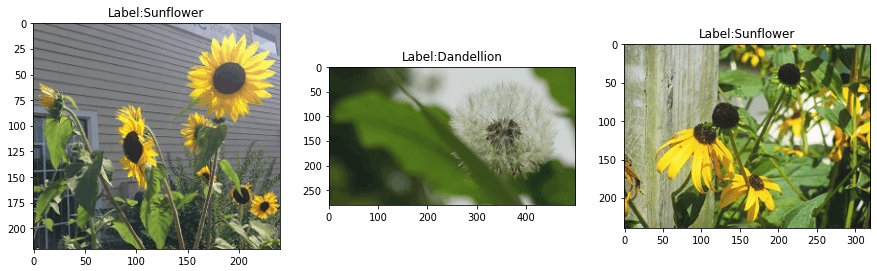
\includegraphics[width=0.65\textwidth]{experiments/datasets/wild-plants.png}
    \caption{Example images from in \textit{Edible wild plants} \cite{edible-wild-plants}}\label{fig:edible-plants-example}
\end{figure}

\subsection{Marvel Heroes}

The dataset consists of pictures from the Marvel Universe franchise. It has 8 classes, and the train/test data split is defined by the authors. Class distribution is proportional between train and test splits. Dataset is fairly balanced with ratio between the least frequently occurring class and the most common class being $1.12$ (detailed class distribution available in appendix \ref{appendix:datasets:marvel}). The total number of images is 3035 (train: 2584, test: 451). Examples from the datasets can be seen in Figure \ref{fig:marvel-example}.

\begin{figure}[ht]
    \centering
    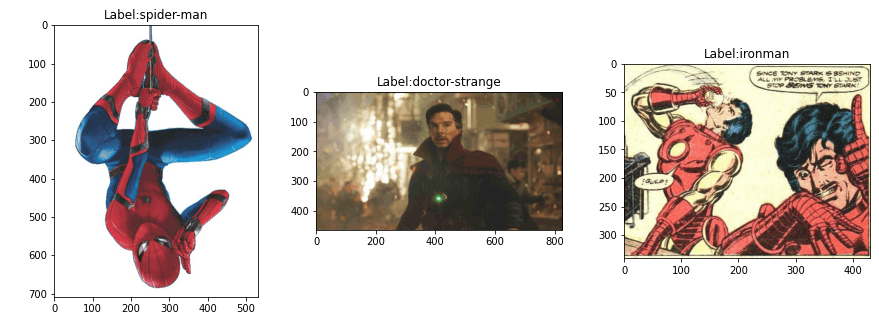
\includegraphics[width=0.65\textwidth]{experiments/datasets/marvel.png}
    \caption{Example images from in \textit{Marvel} \cite{marvel-heroes}}\label{fig:marvel-example}
\end{figure}

\subsection{Plants}

The dataset consists of plant pictures. It has 99 classes, and the train/test data split is defined by the authors. Class distribution is proportional between train and test splits (with the test dataset being slightly more balanced). Dataset is balanced with ratio between the least frequently occurring class and the most common class, being $7$ (detailed class distribution available in appendix \ref{appendix:datasets:plants}). The total number of images is 14670 (train: 13149, test: 1521). Examples from the datasets can be seen in Figure \ref{fig:plants-example}.

\begin{figure}[ht]
    \centering
    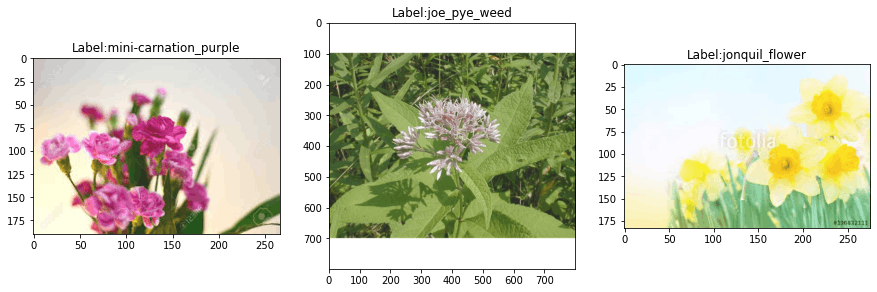
\includegraphics[width=0.65\textwidth]{experiments/datasets/plants.png}
    \caption{Example images from in \textit{Plants} \cite{plants-dataset}}\label{fig:plants-example}
\end{figure}
\section{Models and training}\label{section:models}

This study uses three different model architectures: ResNet 18 \cite{he2015deep}, DenseNet 121 \cite{huang2017densely} and EfficientNet B0 \cite{tan2019efficientnet}. These architectures were selected base on popularity in the data science community and  their availability in popular frameworks. Each model was first pretrained on the ImageNet dataset \cite{imagenet2009}, and fully connected layers from the top of the architecture were removed. There were no further changes to the original structures. On top of the model, a single fully-connected layer was added with the output size matching the number of classes in the particular dataset used for fine-tuning. Fine-tuning is done using Stochastic Gradient Descent (SGD) with momentum \cite{rumelhart1986learning} and Cross-Entropy loss function. Each model was trained for 15 epochs with a decrease of the learning rate (from \textit{0.001} to \textit{0.0001}) after the 7th epoch. Each architecture was trained on every available dataset and every training fraction split of that dataset (train dataset splitting described in section \ref{section:datasets}). In total, $75$ different models were trained for the purpose of the experiments.

\begin{figure}[h]
  \centering
 \begin{subfigure}{.45\textwidth}
    \centering
    \includegraphics[width=\textwidth]{experiments/models/stanford-dogs-f1.png}
    \caption{Stanford Dogs dataset, F1 scores}\label{fig:model-scores-dogs}
\end{subfigure}
 \begin{subfigure}{.45\textwidth}
    \centering
    \includegraphics[width=\textwidth]{experiments/models/food101-f1.png}
    \caption{Food 101 dataset, F1 scores}\label{fig:model-scores-food101}
\end{subfigure}
 \begin{subfigure}{.45\textwidth}
    \centering
    \includegraphics[width=\textwidth]{experiments/models/edible-plants-f1.png}
    \caption{Edible wild plants dataset, F1 scores}\label{fig:model-scores-edible-plants}
\end{subfigure}
 \begin{subfigure}{.45\textwidth}
    \centering
    \includegraphics[width=\textwidth]{experiments/models/marvel-f1.png}
    \caption{Marvel dataset, F1 scores}\label{fig:model-scores-marvel}
\end{subfigure}
 \begin{subfigure}{.45\textwidth}
    \centering
    \includegraphics[width=\textwidth]{experiments/models/plant-data-f1.png}
    \caption{Plants dataset, F1 scores}\label{fig:model-scores-plants}
\end{subfigure}

 \caption{F1 scores achieved by models. Each model was trained using a different fraction of the train dataset and then tested on the full test dataset. We can see a significant drop in the models' performance in most of the datasets. The only outliers are visible in models trained on the \textit{Marvel Heroes} dataset (Fig. \ref{fig:model-scores-marvel}), where scores achieved by the models trained on less data are better in two cases.}\label{fig:model-scores}
\end{figure}

\vspace{\baselineskip}

The results of the training process are aligned with the assumption made (remark \ref{remark:performance-drop-while-train}). Models' performance drops with removing more and more data from the training dataset. There are three exceptions, and all of them are related to the Marvel dataset (see Fig. \ref{fig:model-scores-marvel}). All the architectures observed a slight increase of models' score when were trained on less than $100\%$ of the training dataset. That increase did not last when more data was removed, and the rest of the datasets (Fig. \ref{fig:model-scores-dogs}, Fig. \ref{fig:model-scores-food101}, Fig. \ref{fig:model-scores-edible-plants}, Fig. \ref{fig:model-scores-plants}) did not experience the same phenomenon. Detail results are available in appendix \ref{appendix:models:scores}.
\section{Augmentations}\label{section:augmentation}

To simulate real-world scenarios when evaluating attribution methods on datasets, this work uses the multiple augmentations technique. All described augmentations happen only when the calculation of the SSIM metric is done and never influences the results of the \textit{Infidelity} and the \textit{Sensitivity} measures. 

\begin{wrapfigure}{l}{0.45\textwidth}
  \setlength{\belowcaptionskip}{-62pt}
  \centering
  \includegraphics[width=0.40\textwidth]{experiments/aug/augmentations_example.png}
  \caption{Examples  of  real-world augmentations applied on the input image. Image source: \textit{Stanford Dogs} \cite{stanford-dogs}}\label{fig:augmentation-example}
\end{wrapfigure}\leavevmode

\subsection*{Rotation}\label{section:rotations}

This type of augmentation is one of the simplest augmentations we can apply to any image. It uses the rotation matrix\footnote{Rotation matrix is defined as ${\displaystyle R(\theta )={\begin{bmatrix}\cos \theta &-\sin \theta \\\sin \theta &\cos \theta \\\end{bmatrix}}}$ for a two-dimensional vector, where $\theta$ is an angle we want to rotate} to rotate the position of every pixel and fills the empty space with black pixels. This work is using four rotations \textit{\{$-30^{\circ}$ ,$-15^{\circ}$ ,$15^{\circ}$ ,$30^{\circ}$\}} degrees. Because rotation influences the position of the object on the image, when calculating the SSIM value between two attributions, the same rotation is applied to the attribution of the original image. The result of the applied rotation of $15^{\circ}$ and $-15^{\circ}$ can be seen in Figure \ref{fig:augmentation-example} (bottom row).

\subsection*{Freaky Details}

Freaky details filter \cite{freaky_details} is a method used to enhance details of the input image. It works by creating a copy of the image with inverted color and applying a Bilateral filter \cite{tomasi1998bilateral} to it. After the filter, two images are blended together with a \textit{Vivid Light} mode which blends images base on how "light" is a given pixel. It lightens the pixels that are lighter than 50\% gray color and darkens the pixels that are darker than 50\% gray color. The result of the applied filter can be seen in Figure \ref{fig:augmentation-example} in column 2, row 1. It can be applied iteratively, but for the purpose of experiments, it is only applied once. 

\subsection*{Normalize Local}

Local Normalization filter \cite{normalize_local} is a filter that uses local mean and variance to correct local illumination or shading artifacts. For every pixel at the $(x,y)$ position, we normalize its value:

\begin{equation}
    j_{x,y} = \frac{i_{x,y} - \mu_{loc}(i_{x,y})}{\sigma_{loc}(i_{x,y})}
    \label{eq:local-norm-pixel}
\end{equation}

Where $i_{x,y}$ is a value of the pixel at $(x,y)$ position, $\mu_{loc}$ is a mean value of pixels within a given radius, $\sigma_{loc}$ is a variance of the pixels within a given radius. The radius is a parameter, and in the rest of the experiments, it is always $10$ pixels.

\subsection*{Boost Chromaticity}

Boost Chromaticity filter \cite{boost_chroma} is a filter responsible for changing the "colorfulness" of the pixels. It uses the chromaticity diagram to adjust the chromaticity of the pixels. It usually moves the value of the pixel along with the selected color space to avoid spikes on the chromaticity histogram. In the experiments, the $YCbCr$ color space is used.

\subsection*{Mighty Details}

Mighty details filter \cite{mighty_details} is a filter similar to Freaky details. The main difference is that Mighty details apply smoothing (Gaussian blur) before blending two images.

\subsection*{Sharpen}

Sharpening filter \cite{sharpen} is one of the basic filters available in most image processing software. It uses Gaussian blur to create a blurred version of the original image. A blurred image is then compared with the original image, and if the difference between them is greater than a specific threshold, images are subtracted.
\section{Don’t Augment Me}\label{section:dont-augment-me-definition}

The first part of the experiments relies on the hypothesis that real-world augmentations, which do not cause any significant changes in the augmented image and also do not cause a model to change its prediction significantly, may cause an attribution method to produce significantly different attribution of the augmented image. To measure the difference in attributions quantitatively, I am going to use SSIM \cite{wang2004image} metric. Because quantifying a human visual perception cannot be measured with any known metric and is an active field of research, in addition to the SSIM metric, some of the attributions are going to be presented for qualitative measurement.

\subsection*{Procedure}

To be able to calculate the SSIM metric for the attributions, each dataset and method needs to have a maximum range calculated first. This requires an additional run through all images from the dataset through every model and used method to get a maximum value of attribution assigned by a method for a model. This value is used as a data range in SSIM for all attributions using the same method and model. Lists of calculated maximum attribution values are in appendix \ref{appendix:ssim-ranges}. This range is set for a given experiment and not going to be explicitly mentioned in every one of them unless it is relevant to the change in the setup.

\vspace{\baselineskip}

For an image from the test dataset, a set of augmentations will be applied. Augmentations are defined in Section \ref{section:augmentation}, and all of them are used. The original image, as well as augmented images, are then forwarded through a selected model to get a prediction score. If the prediction score of the augmented image is within the $threshold = 0.05$ that of the original image (non-augmented), then the augmented image is accepted for an attribution comparison. To get the attribution, both the augmented image and the original image are forwarded through a selected attribution method, and resulted attributions are the inputs to the SSIM function. The whole process could be defined as:

\begin{equation}
    SSIM_{x, x_i} = \begin{cases} SSIM(A(F, x), A(F, x_i)) & \text{if } |F(x) - F(x_i)| < 0.05 \\ \text{NaN} & \text{otherwise} \end{cases}
\end{equation}

Where $x$ is an original image, $x_i$ is an augmented image, $F$ is a model, $A$ is an attribution method. There is one exception from this equation, and it occurs when the augmentation is a \textit{rotation} (by any angle). The special case includes applying the same rotation to the attribution from the original image and can be summarized as:

\begin{equation}
    SSIM( R(A( F, x ), \theta), A( F, R(x, \theta)) ))
\end{equation}

The main condition ($|F(x) - F(x_i)| < 0.05$) is still in place, the $x_i$ is replaced by the $R(x, \theta)$, which uses a rotation function $R$ and the angle $\theta$. The same rotation $R$ is applied on the result from the attribution method $A( F, x )$. This fixes the issue of calculating the similarity of rotated attribution to the none rotated attribution. This special case is done under the assumption that rotation of the input image should cause the a similar rotation of the attribution for this image. Comparing attribution from the rotated image to the attribution from the original image would not make sense because the region which is the most important for a prediction is rotated by the $\theta$ angle.

\vspace{\baselineskip}

With all SSIM values calculated, each method will have a mean and the standard deviation value calculated. Additionally, mean and standard deviation values will also be calculated per augmentation. The first calculation should allow comparing the methods, and the second is going to be a supplementary check if there are any exceptions for particular augmentation. The qualitative comparison of the results will include visual rendering of selected examples (original images) along with all augmentations applied to that example. Because the amount of augmentations is far greater than it can be displayed in a comprehensive way, augmentations are going to be split into \textit{rotations} and \textit{filters}. \textit{Rotations} will include all available rotations \ref{section:rotations} (4 in total), and \textit{filters} will include everything except the \textit{rotations} (5 in total). For an example to be considered a valid example, all augmented versions of that example have to achieve class score within the $threshold < 0.05$ from the a score of the original image (non-augmented). This is a more restrictive criterion than the one used for each augmentation separately but removes any potential misinformation on which augmentation is used for valid or not.

\section{Can I Rely On You}\label{section:can-i-rely-on-you-definition}

The second part of the experiments is focused on testing the hypothesis that two of the most popular measures of XAI methods are not reliable when trying to use them to compare methods even within the same data domain. To be able to check if that hypothesis is true, we need to define how the measure should behave for it to be considered reliable.

\begin{definition}\label{def:reliability}
    Given an XAI method $A_1$ and $A_2$ and the measure $S(A)$, measure $S$ is considered reliable, when within the same data domain and model architecture, measures calculated for method $A_1$ always have the same relation to the measures calculated for the method $A_2$.
\end{definition}

\begin{figure}[h]
  \centering
 \begin{subfigure}{.3\textwidth}
    \centering
    \includegraphics[width=\textwidth]{experiments/desc/rel1.png}
    \caption{}\label{fig:rel-measure-1}
\end{subfigure}
 \begin{subfigure}{.3\textwidth}
    \centering
    \includegraphics[width=\textwidth]{experiments/desc/rel2.png}
    \caption{}\label{fig:rel-measure-2}
\end{subfigure}
 \begin{subfigure}{.3\textwidth}
    \centering
    \includegraphics[width=\textwidth]{experiments/desc/unrel1.png}
    \caption{}\label{fig:unrel-measure}
\end{subfigure}

 \caption{An example of reliable measures (Fig. \ref{fig:rel-measure-1}, \ref{fig:rel-measure-2}) and unreliable measures (Fig. \ref{fig:unrel-measure})}\label{fig:reliable-measures-example}
\end{figure}

To illustrate definition \ref{def:reliability}, let us consider an example in Figure \ref{fig:reliable-measures-example}. Each chart represents a relation between the measure score and the models' performance (it could be $F1$ or any valid metric). The ideal measure is shown in Figure \ref{fig:rel-measure-1}, where the relation between values for different attribution methods ($A1$, $A2$, and $A3$) remain the same with the change of models' performance. Changes in the absolute value are not relevant here. The second example (Fig. \ref{fig:rel-measure-2}) is also a valid measure but not as ideal as the first one. Relation between values is changed, but the order of the values is always the same. The third example (Fig. \ref{fig:unrel-measure}) shows the behavior of the unreliable method. The relation between values is changing, and the order in which values for each method are presented is also changing. If there were only two methods in the third example ($A1$ and $A3$), we could assume the measure is reliable. That is the reason why when testing a given measure, we should use more data points.

\subsection*{Procedure}

To properly validate measure Infidelity (Section: \ref{section:infidelity}) and Sensitivity (Section: \ref{section:sensitivity}), each of them has to be tested on every trained model. That gives a total of $375$ different data points for the measure (5 XAI methods $\times$ 5 datasets $\times$ 5 train data fractions $\times$ 3 models). Each data point consists of measures for every sample from the train dataset used for a particular model.

\begin{remark}
The Integrated Gradients (Section \ref{section:ig}) method is not used in this experiment because computing the value of Sensitivity for this method requires more than 11GB of memory.
\end{remark}

Infidelity uses a Gaussian noise with a $\mu = 0$ and $\sigma = 0.003$ to perturb images. Sensitivity creates $10$ perturbed images with the help of the function that samples uniformly random from the $L_{Infinity}$ ball with $0.02$ radius. The results from each data point are processed, and the mean and standard deviation values are calculated. 
	\cleardoublepage
	
	\chapter{Results}\label{chapter:results}
\thispagestyle{chapterBeginStyle}

\vspace{-15mm}
\section{Don’t Augment Me\protect\footnotemark[1]}\label{results:dont-augment-me}

\footnotetext[1]{Results from this section are also part of the paper submitted to the \textit{"Thirty-fifth Conference on Neural Information Processing Systems", NeurIPS 2021} called \textit{"Don’t Augment Me: On the Robustness of Saliency Methods"}. At the moment of writing this thesis, the paper is under the review process. The paper was written in collaboration with Piotr Mazurek.}

\vspace{-1.5\baselineskip}
\begin{figure}[ht]
  \centering
  \includegraphics[width=0.8\textwidth]{results/augment-img/results-all.png}
  \caption{Average SSIM values per attribution method. Each bar represents a methods' mean value of SSIM. These mean values exclude examples when the classification score of the augmented image is outside the $threshold$ of a non-augmented image. Because the score is independent of the attribution method, all mean values are calculated from exactly the same images and augmentations.}\label{fig:SSIM-mean-std}
\end{figure}

\vspace{-1.5\baselineskip}
\begin{wrapfigure}{R}{0.62\textwidth}
%   \setlength{\belowcaptionskip}{-6pt}
 \centering
 \begin{subfigure}{.18\textwidth}
    \centering
    \includegraphics[width=\textwidth]{results/augment-img/20-0-64-rotation-0-harebell_flower-harebell_flower_vert.jpg}
    \caption{Original image}\label{fig:original-harebell}
\end{subfigure}
 \begin{subfigure}{.18\textwidth}
    \centering
    \includegraphics[width=\textwidth]{results/augment-img/20-2-64-rotation--15-harebell_flower-harebell_flower_vert.jpg}
    \caption{Rotation of -15°}\label{fig:rotated-harebell}
\end{subfigure}
 \begin{subfigure}{.22\textwidth}
    \centering
    \includegraphics[width=\textwidth]{results/augment-img/harebell_flower-differences.png}
    \caption{Attribution difference}\label{fig:harebell-differences}
\end{subfigure}

 \caption{Visualisation of attributions for \textit{Harebell Flower} image from Plants \cite{plants-dataset} tested on ResNet18 \cite{he2015deep} trained on 100\% of the training dataset. SSIM value for this pair: \textbf{0.2518}. The difference between attribution of rotated image (Fig. \ref{fig:rotated-harebell}) and the rotated attribution of the original image (Fig. \ref{fig:original-harebell}). Black color indicates the same values, and the white color indicates differences.}\label{fig:xai-harebell-deconv}
\end{wrapfigure}

\hfill \break

After calculating mean SSIM scores per tested method, we can clearly see large discrepancies between XAI methods. The method with the highest average score (Fig. \ref{fig:SSIM-mean-std}) is \textit{Guided GradCAM}, which achieved an average of $0.95$ ($\sigma = 0.05$). On the other hand, we have \textit{Deconvolution} with an average score of only $0.54$ ($\sigma = 0.15$). In terms of SSIM value, this difference is larger than expected, and additional explanation is needed.

\vspace{\baselineskip}

When creating an attribution, the Deconvolution method is using a reverse convolutional operation (building a reverse network, described in Section \ref{section:deconvolution}). Because the output from that network ends with a filter, it creates attributions from basic geometric shapes (see Fig. \ref{fig:xai-harebell-deconv}). This approach has a huge disadvantage when trying to compare attributions of rotated images (unless rotation is defined within a convolutional filter). From a wider perspective, when we look at Figures \ref{fig:original-harebell} and \ref{fig:rotated-harebell}, they look very similar. When we look closer and try to actually compare attribution from Figure \ref{fig:rotated-harebell} with rotated attribution from Figure \ref{fig:original-harebell}, we can see that lines are not aligned with each other (see Figure \ref{fig:harebell-differences}).

\vspace{\baselineskip}

This issue is better visualized when compare the mean value of Deconvolition from Figure \ref{fig:SSIM-mean-rotation} with the value from Figure \ref{fig:SSIM-mean-filters}. There is a clear difference between means (and also standard deviations), with the second Figure having the Deconvolution mean closer to the rest of the methods.

\begin{figure}[ht]
  \centering
  \includegraphics[width=0.8\textwidth]{results/augment-img/rotation-all.png}
  \caption{Average SSIM values per attribution method. Each bar represents a methods' mean value of SSIM. Values used to calculate the mean value are restricted to come only from images augmented by applying rotations. The detailed version of this chart is available in Figure \ref{fig:SSIM-all-rotation}.}\label{fig:SSIM-mean-rotation}
\end{figure}


\begin{figure}[ht]
  \centering
  \includegraphics[width=0.8\textwidth]{results/augment-img/filters-all.png}
  \caption{Average SSIM values per attribution method. Each bar represents a methods' mean value of SSIM. Values used to calculate the mean value are restricted to come only from images augmented by applying filters. The detailed version of this chart is available in Figure \ref{fig:SSIM-all-filters}.}\label{fig:SSIM-mean-filters}
\end{figure}

The values of Guided GradCAM are closest to $1.0$ (see Fig. \ref{fig:SSIM-mean-std}), which would indicate the ideal method (no changes in attributions). A mean score of $0.95$ might be confusing and provide a false sense of trust in the method. A good example can be seen in Figure \ref{fig:xai-tiramisu}. Two attributions have the SSIM score of $0.9357$, but the visual comparison of those two images allows us to see major differences. The main difference is the number of details shown in Figure \ref{fig:norm-tiramisu}. Both images achieve almost the same score, so the augmentation does not cause the model to change its decision. An average score for the Guided GradCAM method is just $0.0143$ away from the score achieved by this example.

\begin{wrapfigure}{R}{0.42\textwidth}
%   \setlength{\belowcaptionskip}{-2pt}
 \centering
 \begin{subfigure}{.2\textwidth}
    \centering
    \includegraphics[width=\textwidth]{results/augment-img/19-0-98-none-Tiramisu-Tiramisu_vert.jpg}
    \caption{Original image}\label{fig:original-tiramisu}
\end{subfigure}
 \begin{subfigure}{.2\textwidth}
    \centering
    \includegraphics[width=\textwidth]{results/augment-img/19-2-98-normalize_local 8,10-Tiramisu-Tiramisu_vert.jpg}
    \caption{Local Norm}\label{fig:norm-tiramisu}
\end{subfigure}

 \caption{Visualisation of attributions done by GradCAM \cite{selvaraju2017grad} for \textit{Tiramisu} image from Food101 \cite{food101} tested on DenseNet121 \cite{huang2017densely} trained on 100\% of the training dataset. SSIM value for this pair: \textbf{0.9357}.}\label{fig:xai-tiramisu}
 \vspace{-38pt}
\end{wrapfigure}

\vspace{\baselineskip}

To provide an overview of the used method, we can look at Figure \ref{fig:attrib-samples}. This overview does not contain all types of examples, which are stored separately and linked in Appendix \ref{appendix:attribution-samples}. Each pair of rows represents a set of augmentations (without rotations) per image per the XAI method. Augmentations names are visible above the examples, and all the predictions of the augmented images are within the $threshold$ of the \textit{"none"} image (first column). This is a slightly more restrictive list than the one used in calculating SSIM values. It is easier to pick examples by searching for the pair of images within the $threshold$ than to find a set of 5 examples where all of them are within the $threshold$. That is why in this list, there are fewer visually different attributions.

\vspace{\baselineskip}

Every set of augmentations contain at least one example where the attribution is significantly different than the original one. Lets start with the Deconvolution (\textit{Rottweiler}). Two augmentations (\textit{Freaky Details} and \textit{Local Norm}) are causing the attribution method to display more details than the original one. Some of those details are related to the dog, but the rest is focusing on the window shutter. A similar problem with focusing on the different parts of the image can be seen in the \textit{Dandellion} example generated with Integrated Gradients \cite{sundararajan2017axiomatic}. Only \textit{Mighty Details} attribution stays the same (visually) when attributions for the rest of augmentations are changing their focus of the plant.

\vspace{\baselineskip}

The main problem with these changes in the attribution is that they are nondeterministic. One augmentation might cause a method to focus on the details more, and the same augmentation might create the opposite behavior when applied on a different image (or even the same image but a different model). Some of the changes are minor and can be ignored (like the two just described), but there are more visually outstanding examples.

\vspace{\baselineskip}

Let us look on the examples from Guided GradCAM \cite{selvaraju2017grad}, GradSHAP \cite{erion2019learning}, and Saliency \cite{simonyan2014deep}. An example attributed by Guided GradCAM changes its attribution significantly when the \textit{Mighty Details} filter is applied. This change is significant enough to change our understanding of what is important for a model in predicting the \textit{sussex\_spaniel} class. The attribution of the original image focuses mostly on the dog's head when the attribution of the augmented image focuses on the whole body. The same applies to the example attributed by GradSHAP. Here, the attribution of the original image points to the dog's nose when four other attributions of the augmented images are pointing to other parts of the animal (like ears and eyes). The example from the Saliency method shows different behavior. This time, when applying the \textit{Local Norm} filter on the image, the attribution ignores some of the details in comparison with the original attribution.

\vspace{\baselineskip}

The most relevant example is that generated with the help of GBP \cite{springenberg2014striving}. In that example, the model predicts the \textit{black\_widow} class for all images. The attribution of most is focused on the scene details and the character of Black Widow. This changes when \textit{Local Norm} is applied, and the attribution starts to display a lot of details of the Hulk character. A shift like that might be dangerous when the understanding of the models' decisions is critical.


\begin{figure}[ht]
  \centering
  \includegraphics[width=0.58\textwidth]{results/augment-img/all_methods_samples.png}
  \caption{Augmentation attribution samples for every method. Samples are selected to all be within the $threshold$ of the original image. Each row represents samples for all augmentations except rotations. More samples available in Appendix \ref{appendix:attribution-samples}}\label{fig:attrib-samples}
\end{figure}

\section{Can I Rely On You}\label{results:can-i-rely}

\subsection{Infidelity}\label{results:infidelity}

Infidelity (see Section \ref{section:infidelity}) was the first measure used in the experiments. This measure is producing results that are highly sensitive to the data domain and have similar values within the same dataset and model (see Figure \ref{fig:resnet-inf}). This forces us to compare values only within the same dataset and model architecture. Additionally, the comparison of values for the Deconvolution method is  impossible, as shown in the same figure. The reason for that is the way how Deconvolution is calculating the value of attribution. Deconvolution is not using a softmax layer in the calculation, and therefore the absolute output attribution might be a couple of orders of magnitude higher than other methods. In the rest of the section, I am going to remove Deconvolution from the comparison.

\begin{figure}[h]
  \centering
    \centering
    \includegraphics[width=\textwidth]{results/metrics/resnet18-infidelity vs acc.png}
    \caption{Infidelity scores on \textit{ResNet18} architecture. All scores are the mean value for the particular model and are related to that models' accuracy (x-axis). Most of the scores for a dataset are within the same range, except for the Deconvolution method (see Section \ref{section:deconvolution}).}\label{fig:resnet-inf}
\end{figure}

Because comparing the mean infidelity values from the combined chart is visually difficult (see Figure \ref{fig:resnet-inf}), a set of sub-charts was created. All sub-charts can be found in Appendix \ref{fig:combined-infidelity}, because the results on all of them are similar in terms of importance. We can discuss the measure using only a selected few (see Figure \ref{fig:inf-metrics-examples}). 

\vspace{\baselineskip}

To check whether the infidelity meets the definition of reliable measure (see Def. \ref{def:reliability}), we need to compare relative changes of the mean scores for a set of methods within the same dataset. As shown in Figure \ref{fig:resnet-inf-marvel}, the measure is not reliable according to the definition of reliable measure. The values of mean infidelity are not consistent between different model versions, and if we look at the \textit{Guided Backprop} method, they even changing from being the best to being the worst (with an increase in the accuracy). The same result can be seen in Figure \ref{fig:efficientnet-inf-edible-plants}, where methods are changing order base on the models' accuracy (e.g. Saliency is starting as the best method, then at around $0.78$ accuracy is considered to be the worst, and at $0.81$ accuracy is the second-best). This proves the hypothesis that Infidelity is not a reliable measure to compare the XAI methods. 

\begin{figure}[h]
  \centering
 \begin{subfigure}{.49\textwidth}
    \centering
    \includegraphics[width=\textwidth]{results/metrics/resnet18-marvel-infidelity vs acc.png}
    \caption{Infidelity scores for \textit{Marvel Heroes} dataset on \textit{ResNet18} architecture}\label{fig:resnet-inf-marvel}
\end{subfigure}
 \begin{subfigure}{.49\textwidth}
    \centering
    \includegraphics[width=\textwidth]{results/metrics/efficientnet-edible-plants-infidelity vs f1-score.png}
    \caption{Infidelity scores for \textit{Edible wild plants} dataset on \textit{EfficientNet B0} architecture}\label{fig:efficientnet-inf-edible-plants}
\end{subfigure}

 \caption{Sample results for Infidelity measure selected for visualizing the behavior of the measure with the change of model performance. Both charts are showing the relation between the mean infidelity on the test dataset and the models' accuracy on the same dataset.}\label{fig:inf-metrics-examples}
\end{figure}

\vspace{\baselineskip}

Another case against using the infidelity can be seen if we draw the standard deviation of the infidelity measure for all models and methods. As shown in Figure \ref{fig:densenet-inf-std}, a standard deviation is usually similar to the mean value. This makes a single value unreliable when trying to compare it with another value. To visualize this unreliability of values, we can pick particular examples from the dataset. If we look at Figure \ref{fig:resnet-inf-96}, we can see that the value of infidelity for two examples indicated that the explanation provided by the GBP method is better (lower value of infidelity). Both examples are calculated using the same image and the same model version, so there is no discrepancy in models' behavior. Analyzing the attributions, we could agree that the GBP method provides a better explanation (Fig. \ref{fig:resnet-inf-96-gbp}) because it shows more details from the input image than Guided GradCAM (Fig. \ref{fig:resnet-inf-96-gradcam}). This kind of example would be perfect when trying to convince that the measure is working correctly, but we can pick another image from the test dataset and use the same model and methods to compare infidelity values. This time the comparison is between values for the \textit{mallow} class (Fig. \ref{fig:resnet-inf-107}). The infidelity value for GradCAM (Fig. \ref{fig:resnet-inf-107-gradcam}) is much lower than the value for GBP (\ref{fig:resnet-inf-107-gbp}), and once again, GBP shows more details from the input image. In this example, infidelity indicates that an explanation from GBP is much worse than an explanation from GradCAM, and this can be argued when looking at the attributions.

\begin{remark}
Indication of which explanation is better is just my subjective opinion. Comparing two explanations is a qualitative problem and can vary base on the person comparing the explanations. Provided examples are here to indicate the issue with values and not give an answer to which one is better.
\end{remark}


\begin{figure}[h]
  \centering
 \begin{subfigure}{.45\textwidth}
    \centering
    \includegraphics[width=\textwidth]{results/metrics/96-gbp.png}
    \caption{Guided Backprop}\label{fig:resnet-inf-96-gbp}
\end{subfigure}
 \begin{subfigure}{.45\textwidth}
    \centering
    \includegraphics[width=\textwidth]{results/metrics/96-gradcam.png}
    \caption{Guided GradCAM}\label{fig:resnet-inf-96-gradcam}
\end{subfigure}

 \caption{Attributions with assigned infidelity and sensitivity values for a given XAI method. All attributions are generated using \textit{ResNet18} trained with 100\% of training data. Results for the class \textit{japanese-knotweed} from \textit{Edible wild plants} \cite{edible-wild-plants}.}\label{fig:resnet-inf-96}
\end{figure}

\begin{figure}[h]
  \centering
 \begin{subfigure}{.45\textwidth}
    \centering
    \includegraphics[width=\textwidth]{results/metrics/107-gbp.png}
    \caption{Guided Backprop}\label{fig:resnet-inf-107-gbp}
\end{subfigure}
 \begin{subfigure}{.45\textwidth}
    \centering
    \includegraphics[width=\textwidth]{results/metrics/107-gradcam.png}
    \caption{Guided GradCAM}\label{fig:resnet-inf-107-gradcam}
\end{subfigure}

 \caption{Attributions with assigned infidelity and sensitivity values for a given XAI method. All attributions are generated using \textit{ResNet18} trained with 100\% of training data.  Results for the class \textit{mallow} from \textit{Edible wild plants} \cite{edible-wild-plants}.}\label{fig:resnet-inf-107}
\end{figure}

\begin{figure}[ht]
  \centering
    \includegraphics[width=\textwidth]{results/metrics/densenet-infidelity vs score - false predictions only - 30 equal size bins.png}
    \caption{Infidelity scores (with standard deviation) on \textit{DenseNet121} architecture. All scores are the mean value for the particular model and are related to that models' predicted scores (x-axis). Each data point is a mean value of the same amount of samples per dataset. Amounts differ between datasets to always split the results into 30 equally-sized bins.}\label{fig:densenet-inf-std}
\end{figure}


\FloatBarrier

\subsection{Sensitivity}\label{results:sensitivity}

The sensitivity (see Section \ref{section:sensitivity}) measure is more complicated in terms of interpreting the result. Unlike infidelity, which suppose to tell us which XAI method is better, sensitivity measure tells us which XAI method is more prone to change its decision with slight perturbation in the input data. We should keep that in mind when discussing this measure. This time, the Deconvolution method is included in the results because the sensitivity does not have the same issue with an absolute value of attribution as infidelity.

\begin{figure}[ht]
  \centering
    \centering
    \includegraphics[width=\textwidth]{results/metrics/resnet18-sensitivity vs acc.png}
    \caption{Sensitivity scores on \textit{ResNet18} architecture. All scores are the mean value for the particular model and are related to that models' accuracy (x-axis).}\label{fig:resnet-sens}
\end{figure}

The combined results for the sensitivity shown in Figure \ref{fig:resnet-sens} differ from those for infidelity in Figure \ref{fig:resnet-inf}. This time the data range is not related to the dataset that much, and we can see a distinction between different XAI methods in the form of colored layers. Based on this example, we can decide which XAI method is the most and the less sensitive to input perturbation. It is even easier when we use values that come from the same dataset (see Figure \ref{fig:sens-metrics-examples}). The order of the mean values for XAI methods is preserved between datasets. Even with a small irregularity in Figure \ref{fig:resnet-sens-food101} between GradCAM and GradSHAP values at the low end of the models' accuracy, we can agree that sensitivity is a far better measure in terms of reliability (Def. \ref{def:reliability}) than infidelity.

\vspace{-12pt}
\begin{figure}[ht]
  \centering
 \begin{subfigure}{.40\textwidth}
    \centering
    \includegraphics[width=\textwidth]{results/metrics/resnet18-food101-sensitivity vs acc.jpg}
    \caption{Sensitivity scores for \textit{Food101} dataset on \textit{ResNet18} architecture}\label{fig:resnet-sens-food101}
\end{subfigure}
 \begin{subfigure}{.40\textwidth}
    \centering
    \includegraphics[width=\textwidth]{results/metrics/resnet18-plant-data-sensitivity vs acc.jpg}
    \caption{Sensitivity scores for \textit{Plants} dataset on \textit{ResNet18} architecture}\label{fig:resnet-sens-plants}
\end{subfigure}

 \caption{Sample results for the Sensitivity measure selected for visualizing the behavior of the measure with the change of model performance. Both charts show the relation between the mean sensitivity on the test dataset and the models' accuracy on the same dataset. More individual charts available in Appendix \ref{appendix:combined-sens}.}\label{fig:sens-metrics-examples}
\end{figure}

\FloatBarrier

Unfortunately, this reliability does not apply when trying to compare values between architectures. Figure \ref{fig:efficientnet-sens} shows a different order of XAI methods according to the mean sensitivity value. Saliency is still the least sensitive method, but the rest of the methods did not keep their position. Comparing the orders between two architectures allows us to confirm that hypothesis saying that this measure is not capable of reliable compare XAI methods is true.

\begin{figure}[ht]
  \centering
    \centering
    \includegraphics[width=\textwidth]{results/metrics/efficientnet-sensitivity vs acc.png}
    \caption{Sensitivity scores on \textit{EfficientNet B0} architecture. All scores are the mean value for the particular model and are related to that models' accuracy (x-axis).}\label{fig:efficientnet-sens}
\end{figure}

As mentioned at the beginning of this section, sensitivity shows how much a method is sensitive to perturbations in the input data. There is a pattern that can be spotted when looking at the generated examples. Usually, the lower the sensitivity score is, the less accurate the attribution appears to be. As an example, let us compare sensitivity scores for three methods shown in Figure \ref{fig:sens-scores-examples}. An example with the highest sensitivity is a GradCAM (Fig. \ref{fig:sens-score-gradcam}, which has less attribution in total. The method with the lowest sensitivity is always the Saliency (Fig. \ref{fig:sens-score-saliency}) which has more noisy attribution than other methods. This might be caused by the way the sensitivity is calculated. The end value is a total change in attribution after applying perturbation. Methods with fewer attributions (working more like edge detectors) are going to have more attribution change because if the edge is changed, then there is a large difference in value. Methods similar to Saliency, even if the attribution changes, it usually does not change that much because of the initial noise. That might explain differences in mean sensitivity between different models. The attributions produced by the same XAI method usually differ between architectures, and therefore the value of sensitivity is different.

\begin{figure}[ht]
  \centering
 \begin{subfigure}{.3\textwidth}
    \centering
    \includegraphics[width=\textwidth]{results/metrics/720-Carrot cake-Carrot cake_vert.jpg}
    \caption{GradCAM}\label{fig:sens-score-gradcam}
\end{subfigure}
 \begin{subfigure}{.31\textwidth}
    \centering
    \includegraphics[width=\textwidth]{results/metrics/243-Beef tartare-Beef tartare_vert.jpg}
    \caption{Deconvolution}\label{fig:sens-score-deconv}
\end{subfigure}
 \begin{subfigure}{.345\textwidth}
    \centering
    \includegraphics[width=\textwidth]{results/metrics/1246-Clam chowder-Clam chowder_vert.jpg}
    \caption{Saliency}\label{fig:sens-score-saliency}
\end{subfigure}

 \caption{Sensitivity scores for different methods produced for \textit{ResNet18} architecture and examples from \textit{Food101} dataset: \textit{Beef tartare} \ref{fig:sens-score-deconv}, \textit{Carrot cake} \ref{fig:sens-score-gradcam}, \textit{Clam chowder} \ref{fig:sens-score-saliency}.}\label{fig:sens-scores-examples}
\end{figure}

\vspace{\baselineskip}

Additionally, we have to look at the standard deviation of the sensitivity scores (Fig. \ref{fig:resnet-sens-std}). This chart significantly differs from the one showing standard deviation for infidelity. The standard deviation for mean sensitivity measure per score shows that some methods (like Saliency) have low variance in sensitivity when methods with more detailed attributions (like GradCAM) have higher variance. That is related to some methods showing less noise in the attributions. The standard deviation also is dependent on the architecture, and sometimes the values of the deviation might vary a lot. A good example is a chart created for EfficientNet B0 architecture in Figure \ref{fig:efficientnet-sens-std}. Some of the values are outside the value range (GradCAM).

\begin{figure}[ht]
  \centering
    \includegraphics[width=\textwidth]{results/metrics/resnet18-sensitivity vs score - true predictions only - 30 equal size bins.png}
    \caption{Sensitivity scores (with standard deviation) on \textit{ResNet18} architecture. All scores are the mean value for the particular model and are related to that models' predicted scores (x-axis). Each data point is a mean value of the same amount of samples per dataset. Amounts differ between datasets to always split the results into 30 equally-sized bins.}\label{fig:resnet-sens-std}
\end{figure}

\begin{figure}[ht]
  \centering
    \includegraphics[width=\textwidth]{results/metrics/efficientnet-sensitivity vs score - true predictions only - 30 equal size bins.png}
    \caption{Sensitivity scores (with standard deviation) on \textit{EfficientNet B0} architecture. All scores are the mean value for the particular model and are related to that models' predicted scores (x-axis). Each data point is a mean value of the same amount of samples per dataset. Amounts differ between datasets to always split the results into 30 equally-sized bins.}\label{fig:efficientnet-sens-std}
\end{figure}
	\cleardoublepage
	
	\chapter{Discussion and Conclusion}\label{chapter:conclusion}
\thispagestyle{chapterBeginStyle}

\vspace{-15mm}
The discussion in this chapter focuses separately on each part of the experiments. This division is due to other aspects of the problem being touched. The first part, named \textit{"Don't Augment Me"}, focuses on the problem with XAI methods, when the second part, titled \textit{"Can I Rely On You"}, discusses a broader problem of being able to compare these methods. The chapter ends with the conclusion and presents the idea of possible future exploration in the field.

\section{Don't Augment Me}

The common practice in designing machine learning models is to use predefined building blocks, and with the evolution of frameworks, it is going to become even more accessible for non-researchers to develop and deploy models. Because explainability is becoming a requirement, some of those developers are going to use available XAI methods base on their popularity. The usual process of understanding the models' decision is to check the input attribution for a set of test examples, and base on that attribution, decide if the model is working correctly. As shown in this thesis, that kind of approach can provide us with insufficient information to understand our model. Real-world examples might provide a different explanation than the ones from the test set (see Figure \ref{fig:augmentation-example} and the \textit{cardigan} attributions for original and locally normalized images).

\vspace{\baselineskip}

The first experiment results gave us an understanding of how the current XAI methods behave when the input of the model is augmented with easily accessible augmentations. Base on similarity comparison, we could deduct that the method with the highest robustness is Guided GradCAM. This method achieved the highest SSIM scores with the lowest standard deviation, but like mentioned in section \ref{results:dont-augment-me}, the GradCAM method is far from being ideal (see Fig. \ref{fig:xai-tiramisu}). Every method tested in this study appears to be influenced by the perturbations that have little to no effect on the models' prediction. This is concerning because the methods' behavior is nondeterministic. When applied to the actual model, we cannot be sure if the result given by the method is the correct one unless we test every single one.

\vspace{\baselineskip}

The positive aspect of the experiments is that the robustness of the method is changing in a minimal way between different types of augmentations. The substantial change is seen only in the case of Deconvolution (see Fig, \ref{fig:SSIM-mean-rotation}), where the method has a significant drop in the performance. The drop was caused by the way Deconvolution presents the attributions and the difference between the attribution of the rotated image and the rotated attribution of the original image. This issue could be fixed by using a different methodology than initially assumed. However, the SSIM metric is not an ideal metric and can be improved to match the human visual perception better. Even with those flaws, the results were consistent across different methods and augmentations.

\section{Can I Rely On You}

Base on results from the first part of the experiments, we can agree that having a reliable and comparable measure is beneficial. With that measure, we could compare existing XAI methods and improve new ones. Two of the most popular XAI methods were tested in the second part of the experiments. The results differed between the methods, and it is better to discuss them separately. 

\vspace{\baselineskip}

Infidelity was the first measure tested against multiple models and datasets. The results showed that this measure is extremely dependent on the dataset, model architecture, and even model performance. It failed the reliability test on any level, and the results showed that values returned by the measure could not be compared even within the same trained model. Even if it has a strong, sensible, theoretical background, the absolute value of infidelity cannot be used to compare the two values. The relative value of infidelity for method A when compared with method B changes within the same model architecture and dataset just after the model performance changes (see Fig. \ref{fig:inf-metrics-examples}). A method that was considered the best (lowest infidelity score) after the model is better trained on the same dataset achieves the worst result. That kind of behavior is unacceptable in the measure. Even values of the infidelity from the same trained model and methods are inconsistent (see a comparison of infidelity values between Fig. \ref{fig:resnet-inf-96} and Fig. \ref{fig:resnet-inf-107}.

\vspace{\baselineskip}

Sensitivity measure achieves far better results than infidelity, but unlike infidelity, it is not a measure of quality but the measure of robustness. As shown in Figures \ref{fig:resnet-sens} and \ref{fig:sens-metrics-examples}, the measure is able to compare different methods within the same model architecture, and there is less value change between different accuracy. However, the absolute value of sensitivity is still a meaningless value because the value changes between architectures. The mean value for the ResNet18 cannot be compared with the value for EfficientNet B0 (compare Fig. \ref{fig:resnet-sens} and Fig. \ref{fig:efficientnet-sens}). The order of methods also differs between different architectures. Base on that information, we can assume that sensitivity could be used as a measure within the same architecture, and because ML practitioners are usually reusing a limited set of predefined architectures, there could be a set of XAI methods that work best for a specific architecture. During the experiments, the sensitivity seems to give the lower scores to the methods with less detailed attributions (see Fig. \ref{fig:sens-scores-examples}). Attribution methods that work more like edge detectors (GBP or GradCAM) tend to receive larger values of sensitivity.

\section{Conclusion}

XAI is still a new branch of the field but already gotten implemented in some of the popular libraries \cite{kokhlikyan2020captum, tensorflow2015-whitepaper}, and even by a top-tier cloud provider \cite{gcp_ig}. Package developers and cloud service providers are doing their best to help the engineers understand their models, but as shown in the number of papers and this thesis, current methods are far from being a ready solution. Without understanding the particular method's drawbacks, the method might provide a false sense of understanding for the developer and cause a severe problem for the end-user.

\vspace{\baselineskip}

As shown in this study, the reliability and robustness of XAI methods are a major issue. Not having a sensible measure to compare those methods is one of the concerns because we as a community are not able to validate if a newly released method is better than the previous one. This also does not help the authors of the methods because they have to rely on qualitative measures, like manual attribution comparison, to determine the quality of their work. This could cause a problem with cherry-picked examples presented in scientific papers. To provide the confirmation that our new method works, we only have to find a handful of examples to include in a paper instead of calculating a numerical value that determines the quality of the method.

\section{Future Work}

This thesis focused mostly on exposing the problem with XAI methods and available measures. With the results, new ideas for improving the current state of the field emerged. One of those ideas is to create a reliable measure for XAI methods which is based on structural similarities of the attribution for visual tasks. SSIM used in this thesis is just a basic structural similarity metric and already have multiple improved version. This should also fix the issue with methods similar to Deconvolution, which had terrible scores on rotated images. Another idea is to improve the measure of infidelity to be able to compare not only the reliability of the method but the quality as well. Eventually, the goal is to create a set of tests integrated with one of the popular XAI frameworks, which can be performed on any method to determine its quality and robustness.
	\cleardoublepage
	
	
	%%%%%%%%%%%%%%%%%%%%%%%%%%%%%%%%%%%%%%%%%%%%%%%%%%%%%%%%%%%%%%%%%%%%%%%%%%%%%%
	%%%%%%%%%%%%%%%%%%%%%%%%%%%%%%% BIBLIOGRAFIA %%%%%%%%%%%%%%%%%%%%%%%%%%%%%%%%%
	%%%%%%%%%%%%%%%%%%%%%%%%%%%%%%%%%%%%%%%%%%%%%%%%%%%%%%%%%%%%%%%%%%%%%%%%%%%%%%

	\pagestyle{bibliographyStyle}
	\bibliographystyle{plabbrv}
	\bibliography{literature}
	\thispagestyle{chapterBeginStyle}
        \addcontentsline{toc}{chapter}{Bibliography}

	\cleardoublepage
	
	%%%%%%%%%%%%%%%%%%%%%%%%%%%%%%%%%%%%%%%%%%%%%%%%%%%%%%%%%%%%%%%%%%%%%%%%%%%%%%
	%%%%%%%%%%%%%%%%%%%%%%%%%%%%%%%%% DODATKI %%%%%%%%%%%%%%%%%%%%%%%%%%%%%%%%%%%%
	%%%%%%%%%%%%%%%%%%%%%%%%%%%%%%%%%%%%%%%%%%%%%%%%%%%%%%%%%%%%%%%%%%%%%%%%%%%%%%
	
    \listoffigures
    
    \listoftables
    
    % \listoflistings
    
	\appendix
	\pagestyle{appendixStyle}
	
	\chapter{Open Science Framework}\label{appendix:osf}
\thispagestyle{chapterBeginStyle}
\label{appendix:source-code}

Source code is available at \url{https://github.com/burnpiro/xai-correlation}. Repository includes detailed instruction on how to run and reproduce experiments. The source code has an additional Wiki page available at \url{https://github.com/burnpiro/xai-correlation/wiki} with some of the results, links to trained models and additional instructions.

\subsection*{Requirements}

\begin{itemize}
  \item Python 3.8
  \item git
  \item Graphic card with at least 11GB of free memory (tested on GForce GTX 1080Ti)
\end{itemize}

\section{Datasets}\label{appendix:datasets}

\subsection{Stanford Dogs}\label{appendix:datasets:stanford-dogs}

\begin{figure}[ht]
  \centering
 \begin{subfigure}{.48\textwidth}
    \centering
    \includegraphics[width=\textwidth]{appendixes/images/dogs-train.png}
    \caption{Train dataset}
\end{subfigure}
 \begin{subfigure}{.48\textwidth}
    \centering
    \includegraphics[width=\textwidth]{appendixes/images/dogs-test.png}
    \caption{Test dataset}
\end{subfigure}

 \caption{Class distribution in \textit{Stanford Dogs}\cite{stanford-dogs} dataset. Data available at \url{http://vision.stanford.edu/aditya86/ImageNetDogs/}.}
\end{figure}

\FloatBarrier

\subsection{Food 101}\label{appendix:datasets:food101}

Data available at \url{https://www.kaggle.com/dansbecker/food-101}. Each class has 750 examples in training dataset and 250 examples in test dataset. 101 classes in total.

\FloatBarrier

\subsection{Edible wild plants}\label{appendix:datasets:edible-plants}

\begin{figure}[ht]
  \centering
 \begin{subfigure}{.48\textwidth}
    \centering
    \includegraphics[width=\textwidth]{appendixes/images/edible-train.png}
    \caption{Train dataset}
\end{subfigure}
 \begin{subfigure}{.48\textwidth}
    \centering
    \includegraphics[width=\textwidth]{appendixes/images/edible-test.png}
    \caption{Test dataset}
\end{subfigure}

 \caption{Class distribution in \textit{Edible wild plants}\cite{edible-wild-plants} dataset. Data available at \url{https://www.kaggle.com/gverzea/edible-wild-plants}.}
\end{figure}

\FloatBarrier

\subsection{Marvel Heroes}\label{appendix:datasets:marvel}

\begin{figure}[hbt!]
  \centering
 \begin{subfigure}{.35\textwidth}
    \centering
    \includegraphics[width=\textwidth]{appendixes/images/marvel-train.png}
    \caption{Train dataset}
\end{subfigure}
 \begin{subfigure}{.35\textwidth}
    \centering
    \includegraphics[width=\textwidth]{appendixes/images/marvel-test.png}
    \caption{Test dataset}
\end{subfigure}

 \caption{Class distribution in \textit{Marvel Heroes}\cite{marvel-heroes} dataset. Data available at \url{https://www.kaggle.com/hchen13/marvel-heroes}.}
\end{figure}

\FloatBarrier

\subsection{Plants}\label{appendix:datasets:plants}

\begin{figure}[ht]
  \centering
 \begin{subfigure}{.4\textwidth}
    \centering
    \includegraphics[width=\textwidth]{appendixes/images/plants-train.png}
    \caption{Train dataset}
\end{subfigure}
 \begin{subfigure}{.4\textwidth}
    \centering
    \includegraphics[width=\textwidth]{appendixes/images/plants-test.png}
    \caption{Test dataset}
\end{subfigure}

 \caption{Class distribution in \textit{Plants}\cite{plants-dataset} dataset. Data available at \url{https://www.kaggle.com/muhammadjawad1998/plants-dataset99-classes?select=Plant_Data}.}
\end{figure}

\FloatBarrier

\section{Models}\label{appendix:models:scores}

Trained models are available at \url{https://drive.google.com/drive/folders/1WVmokp5vaPwOGhpEC6elGVE0aM7fPqNU?usp=sharing}. Step by step instruction on how to train models is available at \url{https://github.com/burnpiro/xai-correlation/wiki/Train-and-Eval-Models}.

\begin{longtable}{|l|l|l|l|r|r|}
\caption{Models' F1 and Accuracy scores}
\label{tab:appendix:models:all-scores} \\\hline
ID &        Dataset &         Model & Data Fraction &     Acc &      F1 \\\hline
0  &  Edible wild plants &      ResNet18 &       100\% &  0.8146 &  0.7671 \\
1  &  Edible wild plants &      ResNet18 &        80\% &  0.7867 &  0.7348 \\
2  &  Edible wild plants &      ResNet18 &        60\% &  0.7709 &  0.7168 \\
3  &  Edible wild plants &      ResNet18 &        40\% &  0.7411 &  0.6634 \\
4  &  Edible wild plants &      ResNet18 &        20\% &  0.5519 &  0.4914 \\\hline
5  &        Food101 &      ResNet18 &       100\% &  0.7650 &  0.7632 \\
6  &        Food101 &      ResNet18 &        80\% &  0.7550 &  0.7532 \\
7  &        Food101 &      ResNet18 &        60\% &  0.7362 &  0.7326 \\
8  &        Food101 &      ResNet18 &        40\% &  0.7146 &  0.7122 \\
9  &        Food101 &      ResNet18 &        20\% &  0.6741 &  0.6689 \\\hline
10 &         Marvel Heroes &      ResNet18 &       100\% &  0.6813 &  0.6798 \\
11 &         Marvel Heroes &      ResNet18 &        80\% &  0.6935 &  0.6923 \\
12 &         Marvel Heroes &      ResNet18 &        60\% &  0.6759 &  0.6693 \\
13 &         Marvel Heroes &      ResNet18 &        40\% &  0.6361 &  0.6301 \\
14 &         Marvel Heroes &      ResNet18 &        20\% &  0.6017 &  0.5960 \\\hline
15 &     Plants &      ResNet18 &       100\% &  0.8895 &  0.8860 \\
16 &     Plants &      ResNet18 &        80\% &  0.8648 &  0.8590 \\
17 &     Plants &      ResNet18 &        60\% &  0.8287 &  0.8240 \\
18 &     Plants &      ResNet18 &        40\% &  0.7912 &  0.7855 \\
19 &     Plants &      ResNet18 &        20\% &  0.7189 &  0.7010 \\\hline
20 &  Stanford Dogs &      ResNet18 &       100\% &  0.7738 &  0.7662 \\
21 &  Stanford Dogs &      ResNet18 &        80\% &  0.7757 &  0.7681 \\
22 &  Stanford Dogs &      ResNet18 &        60\% &  0.7676 &  0.7618 \\
23 &  Stanford Dogs &      ResNet18 &        40\% &  0.7633 &  0.7567 \\
24 &  Stanford Dogs &      ResNet18 &        20\% &  0.7278 &  0.7208 \\\hline
25 &  Edible wild plants &  EfficientNet B0 &       100\% &  0.8067 &  0.7359 \\
26 &  Edible wild plants &  EfficientNet B0 &        80\% &  0.7805 &  0.7253 \\
27 &  Edible wild plants &  EfficientNet B0 &        60\% &  0.7165 &  0.6338 \\
28 &  Edible wild plants &  EfficientNet B0 &        40\% &  0.5760 &  0.5312 \\
29 &  Edible wild plants &  EfficientNet B0 &        20\% &  0.3392 &  0.2713 \\\hline
30 &        Food101 &  EfficientNet B0 &       100\% &  0.8374 &  0.8368 \\
31 &        Food101 &  EfficientNet B0 &        80\% &  0.8253 &  0.8248 \\
32 &        Food101 &  EfficientNet B0 &        60\% &  0.8140 &  0.8131 \\
33 &        Food101 &  EfficientNet B0 &        40\% &  0.7871 &  0.7870 \\
34 &        Food101 &  EfficientNet B0 &        20\% &  0.7395 &  0.7385 \\\hline
35 &         Marvel Heroes &  EfficientNet B0 &       100\% &  0.7119 &  0.7041 \\
36 &         Marvel Heroes &  EfficientNet B0 &        80\% &  0.6918 &  0.6831 \\
37 &         Marvel Heroes &  EfficientNet B0 &        60\% &  0.6892 &  0.6856 \\
38 &         Marvel Heroes &  EfficientNet B0 &        40\% &  0.6493 &  0.6444 \\
39 &         Marvel Heroes &  EfficientNet B0 &        20\% &  0.5831 &  0.5774 \\\hline
40 &     Plants &  EfficientNet B0 &       100\% &  0.8734 &  0.8703 \\
41 &     Plants &  EfficientNet B0 &        80\% &  0.8523 &  0.8487 \\
42 &     Plants &  EfficientNet B0 &        60\% &  0.8218 &  0.8165 \\
43 &     Plants &  EfficientNet B0 &        40\% &  0.7774 &  0.7664 \\
44 &     Plants &  EfficientNet B0 &        20\% &  0.6734 &  0.6422 \\\hline
45 &  Stanford Dogs &  EfficientNet B0 &       100\% &  0.8343 &  0.8289 \\
46 &  Stanford Dogs &  EfficientNet B0 &        80\% &  0.8293 &  0.8253 \\
47 &  Stanford Dogs &  EfficientNet B0 &        60\% &  0.8240 &  0.8187 \\
48 &  Stanford Dogs &  EfficientNet B0 &        40\% &  0.8041 &  0.7972 \\
49 &  Stanford Dogs &  EfficientNet B0 &        20\% &  0.7654 &  0.7549 \\\hline
50 &  Edible wild plants &      DenseNet 121 &       100\% &  0.8777 &  0.8357 \\
51 &  Edible wild plants &      DenseNet 121 &        80\% &  0.8520 &  0.8145 \\
52 &  Edible wild plants &      DenseNet 121 &        60\% &  0.8062 &  0.7502 \\
53 &  Edible wild plants &      DenseNet 121 &        40\% &  0.7718 &  0.7210 \\
54 &  Edible wild plants &      DenseNet 121 &        20\% &  0.6576 &  0.5957 \\\hline
55 &        Food101 &      DenseNet 121 &       100\% &  0.8465 &  0.8447 \\
56 &        Food101 &      DenseNet 121 &        80\% &  0.8356 &  0.8346 \\
57 &        Food101 &      DenseNet 121 &        60\% &  0.8213 &  0.8189 \\
58 &        Food101 &      DenseNet 121 &        40\% &  0.8023 &  0.8005 \\
59 &        Food101 &      DenseNet 121 &        20\% &  0.7585 &  0.7555 \\\hline
60 &         Marvel Heroes &      DenseNet 121 &       100\% &  0.7196 &  0.7127 \\
61 &         Marvel Heroes &      DenseNet 121 &        80\% &  0.6919 &  0.6911 \\
62 &         Marvel Heroes &      DenseNet 121 &        60\% &  0.7164 &  0.7101 \\
63 &         Marvel Heroes &      DenseNet 121 &        40\% &  0.6853 &  0.6739 \\
64 &         Marvel Heroes &      DenseNet 121 &        20\% &  0.6777 &  0.6582 \\\hline
65 &     Plants &      DenseNet 121 &       100\% &  0.9016 &  0.8995 \\
66 &     Plants &      DenseNet 121 &        80\% &  0.8829 &  0.8799 \\
67 &     Plants &      DenseNet 121 &        60\% &  0.8567 &  0.8516 \\
68 &     Plants &      DenseNet 121 &        40\% &  0.8233 &  0.8182 \\
69 &     Plants &      DenseNet 121 &        20\% &  0.7494 &  0.7397 \\\hline
70 &  Stanford Dogs &      DenseNet 121 &       100\% &  0.8290 &  0.8244 \\
71 &  Stanford Dogs &      DenseNet 121 &        80\% &  0.8179 &  0.8130 \\
72 &  Stanford Dogs &      DenseNet 121 &        60\% &  0.8153 &  0.8099 \\
73 &  Stanford Dogs &      DenseNet 121 &        40\% &  0.8042 &  0.7989 \\
74 &  Stanford Dogs &      DenseNet 121 &        20\% &  0.7932 &  0.7846 \\\hline
\end{longtable}

\chapter{Supplementary Results}\label{appendix:supplementary}
\thispagestyle{chapterBeginStyle}
\label{appendix:supplementary-results}

\section{Don't Augment Me - appendix}\label{appendix:dont-augment}

\subsection{SSIM attribution ranges}\label{appendix:ssim-ranges}

\begin{table}[h]
 \centering
  \caption{SSIM ranges for attribution methods for ResNet18}
  \label{tab:ranges-for-resnet}
    \begin{tabular}{|l|lllll|}
    \hline
     \backslashbox{Attribution}{Dataset} & Edible plants & Food 101 & Marvel & Plants &
     Stanford Dogs \\
     \hline
    Deconvolution & 0.784622 & 0.423285 & 0.473029 & 0.682504 & 1.283490\\
    Integrated Gradients & 0.421971 & 1.306827 & 0.611498 & 0.887589 & 1.565911\\
    Saliency & 0.047666 & 0.045500 & 0.067406 & 0.094456 & 0.060711\\
    Grad-Cam  & 0.000047 & 0.000051 & 0.000022 & 0.000085 & 0.000064 \\
    Grad-Shap & 0.145404 & 0.093035 & 0.102947 & 0.285072 & 0.147860 \\
    Guided Backprop & 0.079774 & 0.069185 & 0.050991 & 0.126553 & 0.152545 \\
    \hline
    \end{tabular}
\end{table}


\begin{table}[h]
 \centering
  \caption{SSIM ranges for attribution methods for DenseNet121}
  \label{tab:ranges-for-densenet}
    \begin{tabular}{|l|lllll|}
    \hline
     \backslashbox{Attribution}{Dataset} & Edible plants & Food 101 & Marvel & Plants &
     Stanford Dogs \\
     \hline
    Deconvolution & 4677.117 & 80.11916 & 3037.732 & 1715.939 & 2044.188\\
    Integrated Gradients & 1.099644 & 2.577734 & 0.997656 & 0.816421 & 2.090753\\
    Saliency & 0.068720 & 0.048571 & 0.052243 & 0.068942 & 0.149736\\
    Grad-Cam  & 0.000278 & 0.000187 & 0.000510 & 0.000395 & 0.002106 \\
    Grad-Shap & 0.142074 & 0.119778 & 0.162216 & 0.143393 & 0.345822\\
    Guided Backprop & 0.400560 & 0.218944 & 0.512460 & 0.720738 & 1.565153\\
    \hline
    \end{tabular}
\end{table}

\begin{table}[h]
 \centering
  \caption{SSIM ranges for attribution methods for EfficientNet B0}
  \label{tab:ranges-for-efficientnet}
    \begin{tabular}{|l|lllll|}
    \hline
     \backslashbox{Attribution}{Dataset} & Edible plants & Food 101 & Marvel & Plants &
     Stanford Dogs \\
     \hline
    Deconvolution & 0.078107 & 0.025042 & 0.030603 & 0.055335 & 0.071512\\
    Integrated Gradients & 0.732469 & 5.059399 & 0.810054 & 1.551912 & 2.329165\\
    Saliency & 0.095080 & 0.032253 & 0.043658 & 0.140426 & 0.136111\\
    Grad-Cam  & 0.000028 & 0.000005 & 0.000007 & 0.000042 & 0.000037 \\
    Grad-Shap & 0.464270 & 0.054290 & 0.154112 & 0.280005 & 0.352823\\
    Guided Backprop & 0.068730 & 0.037462 & 0.030622 & 0.066075 & 0.102107\\
    \hline
    \end{tabular}
\end{table}

\subsection{Detailed SSIM results}

\begin{figure}[ht]
  \centering
  \includegraphics[width=\textwidth]{appendixes/images/rotation-ssim.png}
  \caption{Average SSIM values per attribution method and augmentation type (rotations). Each bar represents a methods' mean value of SSIM. Values used to calculate the mean value are restricted to come only from images augmented by applying specific rotations.}\label{fig:SSIM-all-rotation}
\end{figure}

\begin{figure}[ht]
  \centering
  \includegraphics[width=\textwidth]{appendixes/images/filters-ssim.png}
  \caption{Average SSIM values per attribution method and augmentation type (filters). Each bar represents a methods' mean value of SSIM. Values used to calculate the mean value are restricted to come only from images augmented by applying specific filter.}\label{fig:SSIM-all-filters}
\end{figure}

\FloatBarrier

\subsection{Attributions samples}\label{appendix:attribution-samples}

Because the amount of attribution examples is to large to fit them in the appendix, they are available at \url{https://drive.google.com/drive/folders/1Vp3MYRg8j-6ZAfDePeT5kHYPu2Rv6r4t?usp=sharing} (total number of files equals $97990$). File structure is following the pattern \verb|{Augmentation Type}/{Dataset}/{Model version}/{XAI method}|. Each image has a filename containing:

\verb|{index}-{sample id}-{class id}-{augmentation method}-{true class}-{predicted class}.png|

\vspace{5mm}

Combined attribution samples are available at

\url{https://drive.google.com/drive/folders/1lnNQwH3-H1cHiNOEcmnd4OhSScDSuzt0?usp=sharing}.

\begin{figure}[ht]
  \centering
  \includegraphics[width=0.8\textwidth]{appendixes/images/filters-sample.jpg}
  \caption{\textbf{Attribution comparison of inputs with applied filters.} Figure shows three distinct images (\textit{harebell\_flower}, \textit{cardigan}, \textit{pancakes}) with different filters. All attributions done by Guided GradCAM.}\label{fig:filters-samples}
\end{figure}

\begin{figure}[ht]
  \centering
  \includegraphics[width=0.8\textwidth]{appendixes/images/rotation-sample.jpg}
  \caption{\textbf{Attribution comparison of rotated inputs.} Figure shows three distinct images (\textit{harebell\_flower}, \textit{poutine}, \textit{red\_rose}) with different rotations. All attributions done by Guided GradCAM.}\label{fig:rotation-samples}
\end{figure}
\section{Can I Rely On You - appendix}\label{appendix:can-i-rely}

\subsection*{Attribution Examples}\label{appendix:attribution-examples}

Because the amount of attribution examples is to large to fit them in the appendix, they are available at \url{https://drive.google.com/drive/folders/177nMz2Y21Z505Eb5r8NZwAMQoMfX6S5f?usp=sharing} (total number of files equals $23150$). File structure is following the pattern \verb|{{Dataset}/{Model version}/{XAI method}|. Each image has a filename containing:

\verb|{index}-{true class}-{predicted class}.png|

\subsection{Infidelity - combined scores}\label{appendix:combined-inf}

Individual scores can be find at \url{https://drive.google.com/drive/folders/1_0PaXj2QbuW5DyAFjlrKAUjJ_iaoEn9a?usp=sharing}. Folder "\textbf{individual}" contains separated scores per dataset/model. Folder "\textbf{combined}" contains combined scores. Folder "\textbf{confidence}" contains infidelity values with standard deviation values.

\begin{figure}[ht]
  \centering
  \includegraphics[width=\textwidth]{appendixes/images/inf-combined-f1.png}
  \caption{Combined Infidelity scores against F1 scores. Each row represents a dataset, each column represents an architecture (see individual subplot titles)}\label{fig:combined-infidelity}
\end{figure}

\begin{figure}[ht]
  \centering
    \includegraphics[width=\textwidth]{appendixes/images/efficientnet-infidelity vs score - false predictions only - 30 equal size bins.png}
    \caption{Infidelity scores (with standard deviation) on \textit{EfficientNet B0} architecture. All scores are the mean value for the particular model and are related to that models' predicted scores (x-axis). Each data point is a mean value of the same amount of samples per dataset. Amounts differ between datasets to always split the results into 30 equally-sized bins.}\label{fig:efficientnet-inf-std}
\end{figure}


\begin{figure}[ht]
  \centering
    \includegraphics[width=\textwidth]{appendixes/images/resnet18-infidelity vs score - false predictions only - 30 equal size bins.png}
    \caption{Infidelity scores (with standard deviation) on \textit{ResNet18} architecture. All scores are the mean value for the particular model and related to that models' predicted scores (x-axis). Each data point is a meas value of the same amount of samples per dataset. Amounts differ between datasets to always split the results into 30 equally-sized bins.}\label{fig:resnet-inf-std}
\end{figure}

\subsection{Sensitivity - combined scores}\label{appendix:combined-sens}

Individual scores can be find at \url{https://drive.google.com/drive/folders/12eYJSZFMfI2FZhXQSuwJQ6I8w65EU25e?usp=sharing}. Folder "\textbf{individual}" contains separated scores per dataset/model. Folder "\textbf{combined}" contains combined scores. Folder "\textbf{confidence}" contains sensitivity values with standard deviation values.

\begin{figure}[ht]
  \centering
  \includegraphics[width=\textwidth]{appendixes/images/sensitivity-combined-f1.png}
  \caption{Combined Sensitivity scores against F1 scores. Each row represents a dataset, each column represents an architecture (see individual subplot titles)}\label{fig:combined-sensitivity}
\end{figure}

\begin{figure}[ht]
  \centering
    \includegraphics[width=\textwidth]{appendixes/images/densenet-sensitivity vs score - true predictions only - 30 equal size bins.png}
    \caption{Sensitivity scores (with standard deviation) on \textit{DenseNet121} architecture. All scores are the mean value for the particular model and are related to that models' predicted scores (x-axis). Each data point is a mean value of the same amount of samples per dataset. Amounts differ between datasets to always split the results into 30 equally-sized bins.}\label{fig:densenet-sens-std}
\end{figure}
	\cleardoublepage

\end{document}

